\documentclass[12pt,a4paper,oldfontcommands,openright]{memoir}

\usepackage{amsmath}
\usepackage[font=bf]{caption}
\usepackage{fancyhdr}
\usepackage[hidelinks]{hyperref}
\usepackage[left=30mm,right=30mm,top=30mm,bottom=30mm]{geometry}
\usepackage{listings}
\usepackage{multirow}
\usepackage{paralist}
\usepackage{pdfpages}
\usepackage{pifont}
\usepackage{subcaption}
\usepackage{tikz}
\usepackage{titlesec}
\usepackage{url}
\usepackage{wrapfig}
\usepackage{xspace}

% configure header and footer
\pagestyle{fancy}
\fancyhead[LE,CE,RE,RO,CO,LO]{} % remove everything
\fancyhead[RO]{\scriptsize\rightmark} % section name
\fancyhead[LE]{\scriptsize\leftmark} % chapter name
\fancyfoot[C]{\thepage} % page number

% set spacing between lines
\linespread{1.2}

% redefine chapter title
\titleformat{\chapter}[hang]{\vspace*{-6em}\Huge\bfseries}{\thechapter.{ }}{1pt}{\Huge\bfseries}

% use numbers to represent subsections and add them to the table of
% contents
\maxsecnumdepth{subsection}
\maxtocdepth{subsection}

\begin{document}
\sloppy

% ------------------- FRONT PAGE ------------------ %


\includepdf[fitpaper=true, pages=-]{chapters/frontpage/frontpage.pdf}
\cleardoublepage

% -------------- ACKNOWLEDGMENTS ------------ %

\section*{{\em Acknowledgments}}
\label{chap:acknowledgments}
The research described in the contents of this thesis was
supervised by Prof. Stefano Paraboschi (Università degli Studi di
Bergamo), and has received funding from: 2015 Google Faculty Research
Award Program, Horizon 2020 research and innovation programme under
grant agreement No. 825333 (MOSAICrOWN), Horizon Europe research and
innovation programme under grant agreement No. 101070141 (GLACIATION),
and NextGenerationEU programme under grant agreement No. PE00000018
(GRINS).

I would like to thank Prof. Stefano Paraboschi for the guidance during
this journey. My gratitute also goes to my former and present
colleagues of the Security Lab of Università degli Studi di Bergamo:
Marco Abbadini, Enrico Bacis, Michele Beretta, Dario Facchinetti,
Gianluca Oldani, and Marco Rosa, with whom I had the opportunity to
grow by sharing this experience. A final thank is due to all the
people that supported me during my research, since it is thank to them
that the most difficult parts of my journey have been overcome.

\thispagestyle{empty}
\cleardoublepage

% -------------------- DEDICATION ------------------- %

\thispagestyle{empty}
\vspace*{\stretch{1}}
\begin{flushleft}
	\itshape To my family and the friends that supported me\\
\end{flushleft}
\vspace{\stretch{2}}
\cleardoublepage

% --------------- GENERAL MACROS ---------------- %

\newcommand{\seapp}{SEApp\xspace}
\newcommand{\sel}{SELinux\xspace}
\newcommand{\sea}{SEAndroid\xspace}
\newcommand{\dmng}{Dmng\xspace}
\newcommand{\natisand}{NatiSand\xspace}

% ---------------- HIPHENATIONS ----------------- %

% seapp
\hyphenation{iso-lat-ed-process}
\hyphenation{Pack-age-Man-ag-er-Ser-vice}
\hyphenation{SE-Li-nux-MMAC}
\hyphenation{Ac-tiv-i-ty-Man-ag-er-Ser-vice}
\hyphenation{Iso-lat-ed-Ser-vice}

% wasm
\hyphenation{Web-Ass-em-bly}
\hyphenation{stand-a-lone}

% ------------------- ABSTRACT ------------------ %

\pagenumbering{arabic}

\chapter*[Abstract]{Abstract}
\addcontentsline{toc}{chapter}{Abstract}

Over the years operating systems security has greatly evolved and has
been able to address many of the threats originating by an extensive
and varied set of adversaries.

The mitigation of security threats is particularly important for
mobile operating systems, due to their wide deployment and the
confidential information they hold. Focusing on Android, we notice
that components belonging to the same application share access to the
app internal storage and system services. While this may not be an
issue when the developer trusts all the code belonging to their
application, it clearly becomes one when third-party code is included
to achieve monetization and fast-paced development. Thus, we propose
\seapp, a mechanism allowing developers to isolate the internal
components of Android apps and regulate their permissions on a
per-component basis. This is a crucial step to provide strong user
privacy guarantees and meeting data privacy regulations despite the
use of third-party code.

With the research conducted on Android it soon became clear that,
while securing Android apps on the user device was very important,
it was as much important to secure the cloud applications those
applications interact with. Indeed, modern cloud applications can
quickly grow to an intricate tangle of services, and unfortunately
current technologies prove to be overly coarse to effectively restrict
access control of system resources. To address this problem, we propose
an approach that restricts access to file system resources with a
resource-based granularity. Then, we further explore the topic in the
context of WebAssembly runtimes (e.g., Wasmtime and WasmEdge).
Specifically, we highlight the security implications of enabling
access to system resources through the WebAssembly System Interface
(WASI), and identify opportunities for improvement.
Finally, we consider the use of JavaScript (JS) and TypeScript (TS)
for the implementation of cloud applications thanks to JS runtimes
(i.e., Node.js, Deno and Bun). These software securely renders JS code
in an isolated sandbox, however access to system resources and the
execution of native code raise security concerns, since they break the
JS application isolation. To address these security issues, we propose
\natisand, a component for JavaScript runtimes to control the
filesystem, Inter-Process Communication (IPC), and network resources
available to binary programs and shared libraries.

The technologies described in this thesis advance the state of the art
in fine-grained resource protection in mobile and cloud applications.
The implementations have been released under open-source licenses and
can be easily integrated with existing real systems.

\thispagestyle{empty}
\cleardoublepage

% --------------- TABLE OF CONTENTS --------------- %

\renewcommand{\contentsname}{\vspace*{-3em} Table of Contents}
\renewcommand{\listfigurename}{\vspace*{-3em} List of Figures}
\renewcommand{\listtablename}{\vspace*{-3em} List of Tables}

% The asterisk prevents these from showing up in the ToC
\tableofcontents*
\thispagestyle{empty}
\cleardoublepage

\listoffigures*
\thispagestyle{empty}
\cleardoublepage

\listoftables*
\thispagestyle{empty}
\cleardoublepage

% -------------------- CONTENTS ------------------- %

\chapter[Introduction]{Introduction}
\label{chap:intro}
Over the years operating systems security has greatly evolved and has
been able to address many of the threats originating by an extensive
and varied set of adversaries.

The mitigation of security threats is particularly important for
mobile operating systems, due to their wide deployment and the
confidential information they hold. Focusing on Android, which is open
source and more accessible to researchers, we notice that components
belonging to the same application share access to the app internal
storage and system services. So, third-party code included by
developers in their applications for monetization and
fast-paced-development purposes have the same access to internal data
and system services as the rest of the application. This represents a
threat to the security of applications and the privacy of users. Thus,
we propose \seapp, a mechanism allowing developers to isolate the
internal components of Android apps and regulate their permissions on
a per-component basis. As a natural evolution of the security
mechanisms already available in Android, \seapp design requires to
(i) preserve the security of system components, (ii) limit how it
may affect the development of applications, and (iii) minimize the
performance impact. Our evaluations show our proposal meet these
requirements, and \seapp is a crucial step to provide strong user
privacy guarantees and comply to data privacy regulations despite the
use of third-party code. This claim is supported by the current
direction Google is following for the development of its Privacy
Sandbox on Android~\cite{android-privacy-sandbox}.

With the research conducted on Android it soon became clear that,
while securing Android apps on the user device was very important,
it was as much important to secure the cloud applications those
applications interact with. Indeed, modern cloud applications can
quickly grow to an elaborate and intricate tangle of services, and
keeping track of all the moving parts and their security boundaries
can be very challenging. Nevertheless, in order to mitigate the
impact of security incidents companies need to pay close attention
to the security of their cloud applications. Several research works
and industrial standards recommend the integration of least
privilege policies to prevent disruptions such as file system
tampering. Unfortunately current technologies prove to be overly
coarse to effectively restrict access control of system resources.
To address this problem, we propose an approach that restricts access
to file system resources with a resource-based granularity.
Specifically, we provide an instrumentation solution to retrieve all
the file system resources required by an application component. Then,
we demonstrate how this information can be used to create fine-grained
access policies, and introduce sandboxing using recent kernel security
modules, thus strengthening the security boundary of the whole
application.

Even though effective in restricting access to an entire microservice,
the approach above can be further improved by considering the
specifics of emerging technologies that enable finer-grined
compartmentalization of cloud applications. In the context of
WebAssembly runtimes (e.g., Wasmtime and WasmEdge), we highlight the
security implications of enabling access to system resources through
the WebAssembly System Interface (WASI), and identify opportunities
for improvement. Here, not only our approach permits to introduce
fine-grained policies to restrict file system access, it also replaces
error-prone userspace implementations of the security checks (and the
security issues stemming from them) with a unified eBPF
implementation.

In the context of using JavaScript and TypeScript for the development
of cloud applications, we investigate how JS runtimes secure the
applications they host, and identify a few limitations. Modern
runtimes (i.e., Node.js, Deno and Bun) render JavaScript code in a
secure and isolated environment, however access to system resources
and the execution of native code raise security concerns, since they
break the JS application isolation. Developers commonly rely on native
code to speed up the development and execution of their applications
and, despite that, JS runtimes do not provide built-in solutions for
the isolation of native code, so we propose the introduction of
\natisand; a component for JavaScript runtimes to control the
filesystem, Inter-Process Communication (IPC), and network resources
available to binary programs and shared libraries. Our solution is
characterized by a compact, generic architecture that fits nicely with
modern runtimes. Internally, it leverages {\em
  Seccomp}~\cite{seccompbpf} and Linux Security Modules (LSMs), such
as {\em Landlock}~\cite{landlock} and {\em eBPF}~\cite{corbet2014eBPF}
to restrict access to protected resources.

During the research work, considerable attention was dedicated to the
usability, effectiveness, and performance of our proposals. Indeed, in
most of our proposals, we allow developers to take full advantage of
the high level security mechanisms without requiring them to fully
comprehend the advanced security features employed underneath. The
developer is only required to provide a concise and readable policy
file, which details the access privileges available to the components
of their application and may be automatically generated. Moreover, we
provide extensive evaluations showcasing the mitigation capabilities
of our proposals with respect to common use cases and severe CVEs.
Alongside the security guarantees introduced, we evaluate also their
performance footprint, and can confirm the introduction of very
limited overhead with respect to the original unsecure systems and
significant improvements with respect to alternative approaches. To
promote the reproducibility of our experimental evaluations, and
facilitate the integration of our solutions with existing real systems
our prototype implementations are all available open source.

\section{Document structure}

The thesis is organized in six chapters.

\paragraph*{Chapter~\ref{chap:intro}} illustrates the document
structure and the publications that set the basis for this thesis.

\paragraph*{Chapter~\ref{chap:methodology}} showcases the
methodological approach employed to investigate the use of
fine-grained access control technologies to protect resources in
mobile and cloud applications.

\paragraph*{Chapter~\ref{chap:seapp}} describes \seapp~\cite{seapp}, a
proposal that provides developers with a mechanism to isolate the
internal components of Android apps and regulate their permissions on
a per-component basis. This is achieved by first executing components
in dedicated processes, and then restricting access to the app and
system resources with ad hoc \sel policies. Specifically, it is
possible to declare rules to regulate access to both the internal app
storage and system services, which are otherwise shared between all
the application components, including third-party libraries the app
depends upon. This is a crucial step to provide strong user privacy
guarantees despite relying on third-party code to achieve monetization
and fast-paced development of Android applications. The prototype
implements a patch to the Android Open Source Platform (AOSP) to
demonstrate the feasibility, effectiveness and efficiency of the novel
approach.

\smallskip
\noindent The chapter is organized as follows.

\begin{compactitem}
    \item Section~\ref{sect:seapp_introduction} provides an overview
     of how the security architecture of mobile systems evolved with
     the maturity of the ecosystem.
    \item Section~\ref{sect:seapp_andro_sec} introduces the techniques
     currently enforcing access control in Android.
    \item Section~\ref{sect:seapp_motiv} presents the motivation for
     the introduction of intra-app isolation in Android. Specifically,
     a set of use cases is used to showcase the security measures
     introduced by \seapp.
    \item Section~\ref{sect:seapp_lang} details the \seapp policy
     module syntax, and its constraints to ensure proper integration
     of app and system policies.
    \item Section~\ref{sect:seapp_config} illustrates the policy
     configuration files of \sea and how to use them in \seapp.
    \item Section~\ref{sect:seapp_implementation} discusses the
     changes the \seapp implementation introduced in Android platform.
    \item Section~\ref{sect:seapp_performance} presents the
     experimental evaluation, in which we measure both the
     installation time and runtime overhead introduced by \seapp.
    \item Section~\ref{sect:seapp_relwork} discusses the major
     differences between \seapp and other literature proposals.
    \item Section~\ref{sect:seapp_conclusions} concludes the chapter.
\end{compactitem}
\medskip

\paragraph*{Chapter~\ref{chap:dmng}} highlights the limitations of
the cloud technologies available at the time of writing with regard to
fine-grained access control of system resources. Then, it addresses
the problem proposing an approach that restrict application access to
file system resources with a resource-based granularity. To this end,
we develop \dmng, a flexible and intuitive tool that relies on
instrumentation to collect and audit the activity traces generated by
microservices. Finally, we demonstrate how this information can be
used to create fine-grained access control policies and strengthen the
security boundary of the cloud application.

\smallskip
\noindent The chapter is organized as follows.
\begin{compactitem}
    \item Section~\ref{dmng:sect:introduction} presents the challeges
     of securing cloud applications and briefly discusses the state of
     the art to identify opportunities for improvement.
    \item Section~\ref{sect:motivation} discusses the objectives of
     the solution together with its requirements and trust
     assumptions.
    \item Section~\ref{sect:overview} illustrates an overview of the
     approach by highlighting its integration with both staging and
     production environments.
    \item Section~\ref{sect:cloud-instrum} presents two different
     techniques to instrument cloud applications and trace their
     activity.
    \item Section~\ref{dmng:sect:policy} discusses the generation of
     access control policies from activity traces.
    \item Section~\ref{sect:sandbox} details how we implement the
     lightweight enforcement of the policies.
    \item Section~\ref{dmng:sect:exp} presents an empirical
     evaluation of the mitigation capabilities of our approach and
     its performance.
    \item Section~\ref{dmng:sect:related-work} discuss proposals from
     the literature and how they compare to ours.
    \item Section~\ref{dmng:sect:conclusions} concludes the chapter.
\end{compactitem}
\medskip

\paragraph*{Chapter~\ref{chap:wasm}} explores the use of WebAssembly
outside of web browsers thanks to WebAssembly runtimes (e.g., Wasmtime
and WasmEdge). Specifically, it highlights the security implications
of enabling access to system resources through the WebAssembly System
Interface (WASI) and it identifies opportunities for improvement. With
specific regard to file system resources, runtimes must prevent
hostcalls (i.e., functions provided by the runtime to the guest
WebAssembly application) from accessing arbitrary locations. Current
implementations introduce security checks to only permit access to a
predefined list of directories. This approach not only suffers from
poor granularity, it is also error-prone and has led to security
issues. In this chapter we propose to replace the security checks in
hostcall wrappers with eBPF programs, enabling the introduction of
fine-grained per-module policies.

\smallskip
\noindent The chapter is organized as follows.
\begin{compactitem}
    \item Section~\ref{intro} introduces WebAssembly and the
     challenges WebAssembly runtimes are facing with restricting
     access to system resources.
    \item Section~\ref{sect:wasm:threat-model} models the threat
     an attacker can pose to the implementations of WASI in
     WebAssembly runtimes.
    \item Section~\ref{design} details the design of current
     WASI implementations and proposes an alternative approach.
    \item Section~\ref{sec:exp} evaluates the overhead introduced by
     our novel approach in two different WebAssembly runtimes.
    \item Section~\ref{wasm:rel_works} discusses the related work.
    \item Section~\ref{sect:wasm:conclusions} concludes the chapter.
\end{compactitem}
\medskip

\paragraph*{Chapter~\ref{chap:natisand}} considers the use of
JavaScript (JS) and TypeScript (TS) for implementing the backend of
cloud applications. In this setting, the execution of JS code on the
server-side is enabled by JS runtimes (i.e., Node.js, Deno and Bun).
These sophisticated software securely renders JS code in an isolated
sandbox, however access to system resources and the execution of
native code raise security concerns, since they effectively break the
isolation between the JS application and the host OS. Identifying these
clear security issues, this chapter proposes \natisand, a component for
JavaScript runtimes that leverages {\em Landlock}, {\em eBPF}, and
{\em Seccomp} to control the filesystem, Inter-Process Communication
(IPC), and network resources available to binary programs and shared
libraries. We demonstrate the effectiveness and efficiency of our
approach by implementing and integrating it into Deno, a modern,
security-oriented JavaScript runtime.

\smallskip
\noindent The chapter is organized as follows.
\begin{compactitem}
    \item Section~\ref{sect:introduction} presents the development of
     web applications with the use of JavaScript runtimes and their
     limitations with regard to controlling native code access to
     system resources.
    \item Section~\ref{sectbackground} overviews the structure of
     moderm JS runtimes and provides background on the components
     used by \natisand to build the sandbox.
    \item Section~\ref{sect:sci-ffi} motivates the need of
     ad hoc access restrictions for native code highlighting the
     security implications of an otherwise overpermissive behavior.
    \item Section~\ref{sect:design-and-implementation} presents
     \natisand objectives and architecture.
    \item Section~\ref{natisand:sect:policy} details the policy
     structure and explains how to generate its permission rules.
    \item Section~\ref{sect:case-study-deno} showcases the achievement
     of the aforementioned objectives by integrating \natisand into
     the Deno runtime.
    \item Section~\ref{natisand:sect:exp} presents the ability of
     \natisand to mitigate real-world vulnerabilities while
     introducing only a negligible overhead compared to a permissive
     scenario.
    \item Section~\ref{natisand:rel_works} discusses the major
     differences between \natisand and other literature proposals.
    \item Section~\ref{natisand:sect:conclusions} concludes the chapter.
\end{compactitem}
\medskip

\paragraph*{Chapter~\ref{chap:conclusions}} draws the conclusions of
the thesis and discusses future work.

\section{Publications}

This section presents the list of publications authored during the
Ph.D. course that set the basis for this thesis.

\subsubsection*{Articles in journals}

\begin{itemize}
    \nocite{scalable-mondrian}
    \item Sabrina De Capitani di Vimercati, Dario Facchinetti, Sara
        Foresti, Giovanni Livraga, Gianluca Oldani, Stefano
        Paraboschi, Matthew Rossi, Pierangela Samarati.
        ``\textbf{Scalable Distributed Data Anonymization for Large
        Datasets}''. IEEE Transactions on Big Data (TBD), Volume 9,
        Issue 3. IEEE, 2022.
    
    \nocite{k-flat}
    \item Sabrina De Capitani di Vimercati, Dario Facchinetti, Sara
        Foresti, Gianluca Oldani, Stefano Paraboschi, Matthew Rossi,
        and Pierangela Samarati. ``\textbf{Multi-Dimensional Flat
        Indexing for Encrypted Data}''. Under submission.
\end{itemize}

\subsubsection*{Papers in proceedings of international conferences}

\begin{itemize}
    \nocite{dffoprs-percom21}
    \item Sabrina De Capitani di Vimercati, Dario Facchinetti, Sara
        Foresti, Gianluca Oldani, Stefano Paraboschi, Matthew Rossi,
        and Pierangela Samarati. ``\textbf{Scalable distributed data
        anonymization}''. {\em Proceedings of the 2021 IEEE
        International Conference on Pervasive Computing and
        Communications Workshops and other Affiliated Events (PerCom
        Workshops)}. IEEE, 2021.
    
    \nocite{dffoprs-percom21-artifact}
    \item Sabrina De Capitani di Vimercati, Dario Facchinetti, Sara
        Foresti, Gianluca Oldani, Stefano Paraboschi, Matthew Rossi,
        and Pierangela Samarati. ``\textbf{Artifact: Scalable
        distributed data anonymization}''. {\em Proceedings of the
        2021 IEEE International Conference on Pervasive Computing and
        Communications Workshops and other Affiliated Events (PerCom
        Workshops)}. IEEE, 2021.

    \nocite{seapp}
    \item Matthew Rossi, Dario Facchinetti, Enrico Bacis, Marco Rosa,
        and Stefano Paraboschi. ``\textbf{SEApp: Bringing Mandatory
        Access Control to Android Apps.}''. {\em Proceedings of the
        30th USENIX Security Symposium (USENIX Security 21)}. USENIX,
        2021.

    \nocite{ityt}
    \item Enrico Bacis, Dario Facchinetti, Marco Guarnieri, Marco
        Rosa, Matthew Rossi, and Stefano Paraboschi. ``\textbf{I \em
        Told You Tomorrow: Practical Time-Locked Secrets using Smart
        Contracts}''. {\em Proceedings of the 16th International
        Conference on Availability, Reliability and Security (ARES)}.
        ACM, 2021.

    \nocite{dffoprs-globecom2021}
    \item Sabrina De Capitani di Vimercati, Dario Facchinetti, Sara
        Foresti, Gianluca Oldani, Stefano Paraboschi, Matthew Rossi,
        and Pierangela Samarati. ``\textbf{Multi-dimensional indexes
        for point and range queries on outsourced encrypted data}''.
        {\em Proceedings of the 2021 IEEE Global Communications
        Conference (GLOBECOM)}. IEEE, 2021.

    \nocite{cage4deno}
    \item Marco Abbadini, Dario Facchinetti, Gianluca Oldani, Matthew
        Rossi, and Stefano Paraboschi. ``\textbf{Cage4Deno: A
        Fine-Grained Sandbox for Deno Subprocesses}''. {\em
        Proceedings of the 2023 ACM Asia Conference on Computer and
        Communications Security (ASIACCS)}. ACM, 2023.

    \nocite{enhance-wasm-sandbox}
    \item Marco Abbadini, Michele Beretta, Dario Facchinetti, Gianluca
        Oldani, Matthew Rossi, and Stefano Paraboschi.
        ``\textbf{Leveraging eBPF to enhance sandboxing of
        WebAssembly runtimes}''. {\em Proceedings of the 2023 ACM Asia
        Conference on Computer and Communications Security (ASIACCS)}.
        ACM, 2023.
    
    \nocite{natisand}
    \item Marco Abbadini, Dario Facchinetti, Gianluca Oldani, Matthew
        Rossi, and Stefano Paraboschi. ``\textbf{NatiSand: Native Code
        Sandboxing for JavaScript Runtimes}''. {\em Proceedings of the
        26th International Symposium on Research in Attacks,
        Intrusions and Defenses (RAID)}. ACM, 2023.

    \nocite{dmng}
    \item Marco Abbadini, Michele Beretta, Dario Facchinetti, Gianluca
        Oldani, Matthew Rossi, and Stefano Paraboschi.
        ``\textbf{Lightweight Cloud Application Sandboxing}''. {\em
        Proceedings of the 14th IEEE International Conference on Cloud
        Computing Technology and Science (CLOUDCOM)}. IEEE, 2023.

    \nocite{freya-ipfs}
    \item Marco Abbadini, Michele Beretta, Sabrina De Capitani di
        Vimercati, Dario Facchinetti, Sara Foresti , Gianluca Oldani,
        Stefano Paraboschi, Matthew Rossi, and Pierangela Samarati.
        ``\textbf{Supporting Data Owner Control in IPFS Networks}''.
        {\em Proceedings of the 2024 IEEE International Conference on
        Communications (ICC)}. IEEE, 2024.
\end{itemize}


\chapter[Fine-grained Access Control in Android Applications]{Fine-grained Access Control in \\ Android Applications}
\label{chap:seapp}
% \newcommand{\seapp}{SEApp\xspace}

%tabularx width
\newcolumntype{s}{>{\hsize=.5\hsize}X}

%general
% \newcommand{\sel}{SELinux\xspace}
% \newcommand{\sea}{SEAndroid\xspace}

% files 
\newcommand{\filecontexts}{\texttt{file\_contexts}\xspace}
\newcommand{\genfscontexts}{\texttt{genfs\_contexts}\xspace}
\newcommand{\propertycontexts}{\texttt{property\_contexts}\xspace}
\newcommand{\servicecontexts}{\texttt{service\_contexts}\xspace}
\newcommand{\seappcontexts}{\texttt{seapp\_contexts}\xspace}
\newcommand{\macpermissions}{\texttt{mac\_permissions.xml}\xspace}
\newcommand{\initrc}{\texttt{init.rc}\xspace}
\newcommand{\manifest}{\texttt{AndroidManifest.xml}\xspace}
\newcommand{\sepolicy}{\texttt{sepolicy.cil}\xspace}
\newcommand{\fstab}{\texttt{fstab}\xspace}

% file tags
\newcommand{\process}{\texttt{android:process}\xspace}
\newcommand{\seinfo}{\texttt{seinfo}\xspace}
\newcommand{\mlstrustedsubject}{\texttt{mlstrustedsubject}\xspace}

% file extensions
\newcommand{\te}{\texttt{.te}\xspace}

% directories
\newcommand{\apkpolicydir}{\texttt{policy}\xspace}
\newcommand{\dataselinuxdir}{\texttt{/data/selinux/packageName}\xspace}
\newcommand{\dataappdir}{\texttt{/data/data/packageName}\xspace}
\newcommand{\dataselinux}{\texttt{/data/selinux}\xspace}

% partitions
\newcommand{\selinuxfs}{\texttt{selinuxfs}\xspace}
\newcommand{\system}{\texttt{/system}\xspace}
\newcommand{\product}{\texttt{/product}\xspace}
\newcommand{\vendor}{\texttt{/vendor}\xspace}
\newcommand{\odm}{\texttt{/odm}\xspace}
\newcommand{\dev}{\texttt{/dev}\xspace}
\newcommand{\sys}{\texttt{/sys}\xspace}
\newcommand{\data}{\texttt{/data}\xspace}
\newcommand{\proc}{\texttt{/proc}\xspace}
\newcommand{\selinuxfsfull}{\texttt{/sys/fs/selinux}\xspace}

% capabilities
\newcommand{\dacoverride}{\texttt{DAC\_OVERRIDE}\xspace}
\newcommand{\dacreadsearch}{\texttt{DAC\_READ\_SEARCH}\xspace}

% selinux stmt
\newcommand{\typetransition}{\texttt{typetransition}\xspace}
\newcommand{\allow}{\texttt{allow}\xspace}
\newcommand{\typeattribute}{\texttt{typeattribute}\xspace}
\newcommand{\typeattributeset}{\texttt{typeattributeset}\xspace}
\newcommand{\typebounds}{\texttt{typebounds}\xspace}

% selinux permissions
\newcommand{\relabelfrom}{\texttt{relabelfrom}\xspace}
\newcommand{\relabelto}{\texttt{relabelto}\xspace}
\newcommand{\dyntransition}{\texttt{dyntransition}\xspace}
\newcommand{\setcurrent}{\texttt{setcurrent}\xspace}

% selinux types
\newcommand{\isolatedapp}{\texttt{isolated\_app}\xspace}
\newcommand{\untrustedapp}{\texttt{untrusted\_app}\xspace}
\newcommand{\untrustedapptmpfs}{\texttt{untrusted\_app\_tmpfs}\xspace}
\newcommand{\appdatafile}{\texttt{app\_data\_file}\xspace}
\newcommand{\initdomain}{\texttt{init}\xspace}
\newcommand{\kernel}{\texttt{kernel}\xspace}

% certificates name
\newcommand{\platform}{\texttt{platform}\xspace}
\newcommand{\media}{\texttt{media}\xspace}
\newcommand{\net}{\texttt{network\_stack}\xspace}

% components, services, classes, functions, libraries
\newcommand{\init}{\textit{init}\xspace}
\newcommand{\restorecon}{\textit{restorecon}\xspace}
\newcommand{\restoreconc}{\textit{restorecon.c}\xspace}
\newcommand{\servicemanager}{\textit{servicemanager}\xspace}
\newcommand{\binder}{\textit{Binder}\xspace}
\newcommand{\zygote}{\textit{Zygote}\xspace}
\newcommand{\ams}{\textit{ActivityManagerService}\xspace}
\newcommand{\installd}{\textit{installd}\xspace}
\newcommand{\libselinux}{\textit{libselinux}\xspace}
\newcommand{\systemserver}{\textit{SystemServer}\xspace}
\newcommand{\pms}{\textit{PackageManagerService}\xspace}
\newcommand{\forkandspecialize}{\textit{Zygote.forkAndSpecialize()}\xspace}
\newcommand{\secilc}{\textit{secilc}\xspace}
\newcommand{\setcontext}{\textit{selinux\_android\_setcontext}\xspace}
\newcommand{\restoreconpkgdir}{\textit{selinux\_android\_restorecon\_pkgdir}\xspace}
\newcommand{\restorecond}{\textit{restorecond}\xspace}
\newcommand{\ioctl}{\textit{ioctl}\xspace}
\newcommand{\loadpolicy}{\textit{selinux\_android\_load\_policy}\xspace}
\newcommand{\systemservice}{\textit{SystemService}\xspace}
\newcommand{\contentprovider}{\textit{ContentProvider}\xspace}
\newcommand{\activity}{\textit{Activity}\xspace}
\newcommand{\service}{\textit{Service}\xspace}

% circle shapes
\DeclareRobustCommand{\whitecircle}[1]{\tikz[baseline=-0.3em]{
		\node[shape=circle,scale=0.6,draw,inner sep=2pt] (char) {#1};}}
\DeclareRobustCommand{\blackcircle}[1]{\tikz[baseline=-0.3em]{
		\node[shape=circle,scale=0.6,fill=black,text=white,draw,inner sep=2pt] (char) {#1};}}

% listing style for policy files
\lstdefinelanguage{policyfile}{
	sensitive=true,
	keywords={},
	morecomment=[f][\color{blue}][0]{;},
}

% break url on multiple lines
\def\UrlBreaks{\do\/\do-}

\definecolor{background}{HTML}{EEEEEE}

\lstset{
	xleftmargin=3mm,
	basicstyle=\small\ttfamily,
	numbers=left,
	numberstyle=\scriptsize,
	stepnumber=1,
	numbersep=8pt,
	frame=lines,
	backgroundcolor=\color{background},
	breaklines=true,
}


\section{Introduction}
\label{sect:seapp_introduction}

Security in operating systems has greatly evolved and has been able to
address many of the threats originating by an extensive and varied
collection of adversaries.

The mitigation of security threats is particularly important
for {\em mobile operating systems}, due to their wide deployment and
the confidential information they hold.

Both Android and iOS have seen significant investments toward the
realization of advanced security techniques, which have led to a great
increase in the level of protection offered to
users~\cite{seapp_tapsm_m}.  The strength of security and the value of
protected resources is testified, for instance, by the payouts
associated with working exploits in markets like
Zerodium~\cite{seapp_zerodium}, where the payouts for mobile operating
systems are the highest\footnote{At the time of writing, US\$2.5M and
  US\$2M are paid for a zero click solution able to subvert the
  security of Androd and iOS, respectively. }.

A peculiar threat that characterizes mobile operating systems is the
need to balance on one side the high sensitivity of the information,
and on the other hand the need for users to install into the system a
large number of applications (called simply {\em apps} in this domain)
often produced by unknown developers, which may hide malicious
functions.  A first level of protection is offered, both in iOS and
Android, by a preliminary screening of apps before they are made
available on the platform market~\cite{seapp_playprotect} or installed
to a device, but this approach cannot provide a strong guarantee.
Security mechanisms internal to the operating system are needed in
order to constrain the apps to only operate within the boundaries
specified by the device owner at installation time.

The approach used in the design of mobile operating systems considers
as the first requirement the protection of system resources.  Focusing
on Android, which is open source and more accessible to researchers,
we notice a significant evolution in its internal security
architecture.  This architecture is quite rich and consists of many
security measures~\cite{seapp_10.1145/2046707.2046779,seapp_tapsm_m}.
In this environment, we specifically look at the role of SELinux.
SELinux implements the {\em Mandatory Access Control} (MAC) mechanism,
which relies on a system-level policy to declare the operations that a
process can execute over a resource based on the security labels
associated with them.  Compared to classical {\em Discretionary Access
  Control} (DAC), still used in Android in an extensive way, MAC is
more rigid and provides stronger guarantees against unwanted
behaviors.  When SELinux was introduced into Android 4.3 in 2013 (see
Figure~\ref{fig:seapp_mac_evolution}), it used a limited set of system
domains and it was mainly aimed at separating system resources from
user apps.  In the next releases, the configuration of SELinux has
progressively become more complex, with a growing set of domains
isolating different services and resources, so that a bug or
vulnerability in some system component does not lead to a direct
compromise of the whole system.

The introduction of SELinux into Android has been a clear success.
Unfortunately, the stronger protection benefits do not extend to
regular apps which are assigned with a single domain named
\untrustedapp.  Since Android 9, isolation of apps has increased with
the use of categories, which guarantees that distinct apps operate on
separate security contexts.  Our proposal, \pap, builds upon the
observation that giving app developers the ability to apply MAC to the
internal structure of the app would provide more robust protection
against other apps and internal vulnerabilities.

%%% Local Variables: 
%%% mode: latex
%%% TeX-master: "../../../main.tex"
%%% reftex-default-bibliography: "../../../bib/biblio.bib"
%%% End:
\section{Android security for apps}\label{sect:seapp_andro_sec}

One of the major requirements considered in the design of mobile
operating systems is the need to constrain the ability of apps to
manipulate the execution environment.  Apps may hide functions that
are meant to gain system privileges or capture valuable information
from other apps.  Compared to classical desktop operating systems,
there is greater reliance on the use of apps to access resources or
get services, with more attention paid to limit the ability of apps to
operate in the system.  Advancements in this context can have an
impact on how security for applications is managed in other
domains~\cite{seapp_sok_android}.

\begin{figure}[t]
	\begin{center}
		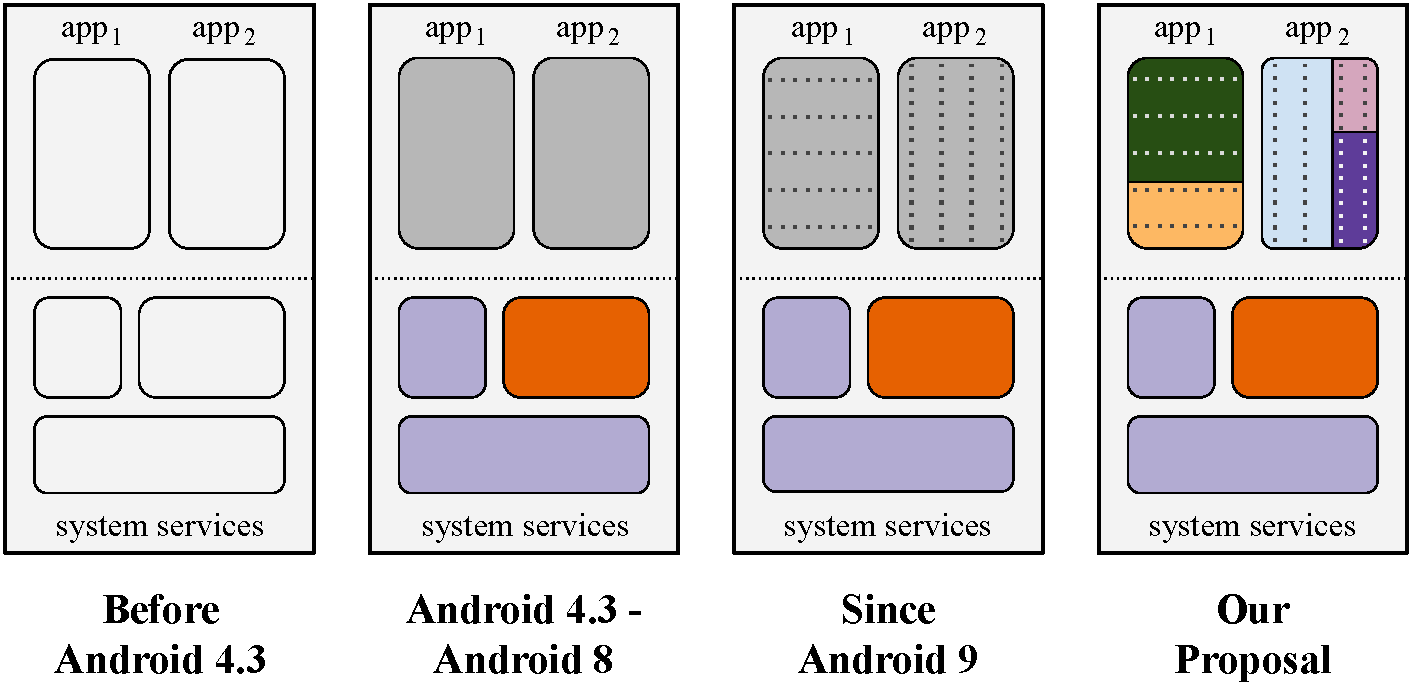
\includegraphics[width=\columnwidth]{chapters/seapp/figs/mac-evolution}
	\end{center}
	\caption[Evolution of the MAC policy in Android]{\label{fig:seapp_mac_evolution} Evolution of the MAC policy
          in Android.  Before 4.3, MAC was not used. Starting with 4.3,
          MAC protects system components. Since 9, categories offer
          rigid MAC protection for apps. Our proposal offers flexible
          MAC protection to apps.}
\end{figure}

The basic principle adopted to manage the threat introduced by apps is
the design of a {\em sandbox}, a restricted environment for app
execution, where anomalous actions by the app are not able to access
resources beyond what has been authorized at app installation time.
The sandbox can be considered a realization of the ``least privilege''
security principle.

The construction of the app sandbox is based on three access control
mechanisms: Android permissions~\cite{seapp_andro_perm,
  seapp_10.1145/2046707.2046779,seapp_10.1145/2335356.2335360},
Discretionary Access Control
(DAC)~\cite{seapp_10.1145/3134600.3134638}, and Mandatory Access
Control (MAC)~\cite{seapp_dacmac}; each of them roughly aligning with
how users, developers, and the platform grant consent, respectively.

Permissions restrict access to sensitive data and services.  In
the \manifest~\cite{seapp_andro_man}, each app statically lists the
Android permissions needed to fully operate.  Not all of them may be
granted; depending on the threat they pose from a security and privacy
standpoint, they may be granted as part of the installation procedure,
or prompted to the user when the app needs them.

DAC restricts access to resources based on user and group identity.
By assigning each application a unique UNIX user ID (UID) and a
dedicated directory, Android isolates apps from each other and from
the system.  However, UID sandboxing has a number of shortcomings.  As
an example, processes running as root are not subject to these
restrictions.  For this reason, when such a process is misbehaving,
for instance due to a bug, it can access private app data files.  DAC
discretionality itself is a problem.  Indeed, as apps and system
processes could override safe defaults, they are more susceptible to
dangerous behavior, such as leaking files or data across security
boundaries via IPC or fork/exec.  Despite its deficiencies, UID
sandboxing is still the primary enforcement mechanism that separates
apps from each other, establishing the foundation upon which further
sandbox restrictions have been built.

MAC dictates which actions are allowed based on the security policy
defined by the system.  Specifically, only actions explicitly granted
by the policy are permitted.  To decide whether to permit or deny an
action, a set of policy rules concerning the {\em security contexts}
(i.e., collections of security labels that classify resources) of the
involved parties is evaluated.

In Android, MAC is implemented using \sea, a set of kernel
modifications part of the Linux Security Module (LSM)
framework~\cite{seapp_lsm_fra}.  Since its first introduction with the
Security Enhanced Android (\sea) project~\cite{seapp_seandroid}, \sel
has been extensively applied to protect system components.  Initially,
it was used to assert the security model requirements during
compatibility testing, then its usage grew further at each release.
In the current version Android 11, \sel is also used to isolate the
rendering of untrusted web content (by the \isolatedapp domain), to
restrict \ioctl system calls~\cite{seapp_restrioctly}, thus limiting
the reachability of potential kernel vulnerabilities, and to support
multi-user separation and app sandboxing with \sel categories.  This
last aspect permits to enforce app separation both at DAC and MAC.
Android dynamically assigns categories to apps during app
installation, so that: (i) an app running on behalf of a user cannot
read or write files created by the same app on behalf of another user
(since Android 6 \cite{seapp_android6_per_user}); and, (ii) an app
cannot read or write files created by another app (since
Android~9\cite{seapp_android9_per_app}).  Before Android~9, this
separation was only enforced at DAC level.  This overlap of security
measures is of extreme relevance to the enforcement of the Android
Security Model and our proposal moves in the same direction.  To
bypass these protections, a process should be granted root
permissions, \dacoverride or \dacreadsearch, and run as SELinux
\mlstrustedsubject; only a few critical system services run in this
configuration.

Android restricts the \sel implementation to the policy enforcement,
ignoring most policy management functions.  The motivation is that the
system policy only changes between releases, therefore support to
runtime changes is not needed.

%%% Local Variables: 
%%% mode: latex
%%% TeX-master: "../../../main.tex"
%%% reftex-default-bibliography: "../../../bib/biblio.bib"
%%% End:

\section{Motivation}\label{sect:seapp_motiv}

As discussed above, \sel and the MAC support have been a crucial
factor in the realization of a secure design and the construction of a
robust app sandbox.  A limitation of the current design is that this
is the only way that apps can benefit from MAC support.  There is
currently no option to let the app developer control the use of the
MAC level, as only platform, vendor, ODM and OEM developers are
allowed to introduce new policy
segments~\cite{seapp_sea_compatibility}.  Our solution overcomes this
limitation, giving the application developer the power to specify new
\sel types and associated permissions.

\subsection{Use cases}\label{sect:seapp_use-cases}
We envision several scenarios that justify the use of \pap.  Many of
them have been previously considered by researchers as motivations for
the introduction in Android of dedicated
components~\cite{seapp_10.1145/2976749.2978333,
  seapp_10.1145/3292006.3300027, seapp_10.1145/3133956.3134064}.

In this section, we give a tour of \pap capabilities using a showcase
app\footnote{The showcase app is available in the \pap repository
  along with the set of modifications to the AOSP.}.  The architecture
of the showcase app is shown in Figure~\ref{fig:seapp_showcase}. Our
description is based on three use cases: fine-granularity in access to
files, fine-granularity in access to services, and isolation of
vulnerability prone components.  Each of the use cases emphasizes the
intra-app security features introduced by \pap.  A dedicated
description, along with policy files that show concretely how to
enforce these use cases, appears in the
Appendix~\ref{appendix:seapp_analysis}; we provide there a technical
demonstration of how \pap can provide protection against a number of
common security problems in Android
apps~\cite{seapp_common_play_protect_vulnerabilites} that were
implemented in the showcase app.

\begin{figure}[h]
	\centering
	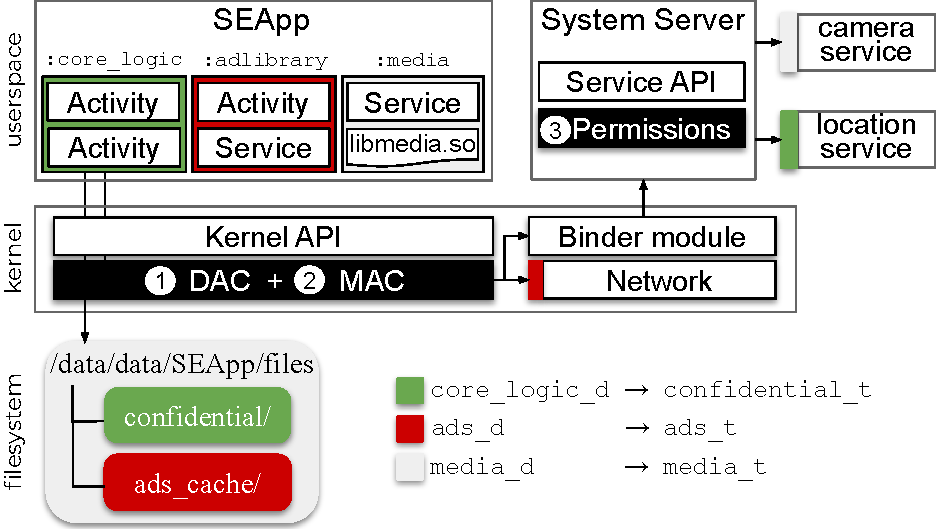
\includegraphics[width=0.8\columnwidth]{chapters/seapp/figs/seapp_showcase_app}
	\caption{\label{fig:seapp_showcase} Security Enhanced App}
\end{figure}

\subsubsection{Fine-granularity in access to files}

Android apps can collect data from multiple sources, and the system
provides many options to store it.  The default one is {\em Internal
  Storage}: a filesystem region, located at \dataappdir, reserved to
each package.  Its content is available to all app's internal
components and inaccessible to any other app.  Since data can be
extremely sensitive, the developer may be interested in restricting
its visibility to only some internal components, labeling sensitive
and non-sensitive data with distinct \sel types (use case 1).  Yet, in
the current Android security model, apps do not have the option to
assign distinct MAC labels to different resources, as all internal
files are labeled \appdatafile.  \pap allows the developer to
introduce dedicated types, and to organize the app's structure with a
separation between components managing non-sensitive data and those
requiring access to sensitive data.  The sensitive components will be
associated with a more stringent MAC domain.
Figure~\ref{fig:seapp_showcase} shows an example in which the {\em
  confidential} files are made accessible to {\em :core\textunderscore
  logic} processes and inaccessible to any other process.

In Appendix~\ref{appendix:seapp_uc1} we give a demonstration of how {\em
  confidential} files are made inaccessible to non-confidential
components in the presence of a path traversal vulnerability.


\subsubsection{Fine-granularity in access to services}

Often developers introduce into their applications code coming from
external sources, which they do not fully trust~\cite{seapp_7958574,
  seapp_10.1145/2414456.2414498, seapp_demetriou2016free}.  For
instance, a common need of app developers is to get revenue from their
apps and a simple approach is to include an Ad delivery library within
the app.  The library is a relatively complex piece of code, with
local computation necessities and the need to manage a dialogue with
remote servers.  The app developer is clearly interested in supporting
the execution of the library, but may want to have guarantees that the
library cannot abuse the access privileges granted by the user to the
whole application sandbox (use case 2).  A common concern is
preventing access to system services such as {\em location}.  These
requirements can be managed by \pap with the definition of a separate
MAC domain for the library.  The process managing the delivery of Ads
will be associated with this domain, which will provide only the
necessary privileges to access the dedicated resources needed for the
library execution.  \sel will then guarantee the confinement of the
library, preventing access to the location service even if the
\texttt{ACCESS\textunderscore FINE\textunderscore LOCATION} permission
is granted to the app.  Figure~\ref{fig:seapp_showcase} shows an
example in which the {\em :adlibrary} process is granted access to the
network but is prevented from accessing \texttt{location service}.

In Appendix~\ref{appendix:seapp_uc2} we give a demonstration of how
the showcase app can support the execution of the Unity
Ads~\cite{seapp_unityads} framework with a dedicated \sel domain. We
also describe in detail how \pap prevents a malicious component, which
was deliberately injected by us into the library process, to capture
the device location.


\subsubsection{Isolation of vulnerability prone
  components}\label{sect:seapp_int_comp_isolation}

App developers often have to consider that the input provided to the
app can come from untrusted sources.  A typical example is the
rendering of complex Javascript code performed by WebView.  The
solution currently offered by Android is to execute these potentially
dangerous actions within a sandbox using {\em isolatedprocess}, i.e.,
a special process that is isolated from the rest of the system and has
no permissions of its own~\cite{seapp_isolatedprocess_perm}.  It runs
under a dedicated UID and \sel domain, and it can only interact with a
restricted number of services~\cite{seapp_isolated_app_te}.

A common need of app developers is to take advantage of complex media
or processing libraries, components that are not considered malicious,
but due to their size and complexity are more likely to have security
bugs.  The developer is then interested in isolating these potentially
vulnerable components (use case 3).  {\em Isolatedprocess} offers a
high protection level in Android, however, its use imposes several
restrictions on the developers.  For instance, {\em isolatedprocess}
cannot perform many of the core Android IPC functions, and the only
way to interact with it is through the bound service
API~\cite{seapp_bound_service_api}.  Also, {\em isolatedprocess} can
only access already open app files received over Binder.  Another
shortcoming is that each invocation of an {\em isolatedprocess}
requires the creation of a new process.  If a series of requests are
made by the app, the performance impact can be significant.  \pap
offers an easier way to do this compared to {\em isolatedprocess}, as
it permits to assign a domain to the process in which the component is
executed, and then configure the required permissions at MAC level.
In terms of performance, the management of multiple requests does not
require the system to activate a new process with a new UID and a
dedicated \sel category.  Figure~\ref{fig:seapp_showcase} shows how to
confine the {\em :media} component.

In Appendix~\ref{appendix:seapp_uc3} we give a demonstration of how
the showcase app can support the execution of media components relying
on a native library in a dedicated process. We also describe how the
developer can leverage \pap to prevent the code of the library from
the execution of unwanted or unintended operations, like opening a
network connection.


\subsection{Modular app compartmentalization}

The motivations presented above become more frequent as apps increase
their size and complexity, and several important apps see a continuous
increase in these parameters.  For instance, Facebook Messenger
version 285 contains more than 500 components and WhatsApp Messenger
version 2.20 more than 300.  This increase in size and the need to
manage it is testified by the development of App
Bundles~\cite{seapp_app_bundles}, Android's new, official publishing
format that offers a more efficient way to build and release modular
applications.

In these large and modular apps, developers find it difficult to fully
control which components of an app are using sensitive
data\footnote{The topic was explicitly considered
  in~\cite{seapp_burke_interview}, an interview with Android's VP of
  Engineering.}.  The availability of a solution such as \pap can
greatly reduce such risk.  A better compartmentalization can reduce
the impact of internal vulnerabilities in modular apps, since each
module can be associated with a dedicated policy fragment.  From a
security and software engineering standpoint, \pap permits to separate
the activities of security policy maintenance and development of new
features.

\subsection{Compatibility with Android design}

Looking at the evolution of Android, it is clear that our proposal is
consistent with the evolution of the operating system and the desire
of its designers to let app developers have access to an extensive and
flexible collection of security tools.  The major obstacles, as
perceived by OS developers, on offering to app developers the use of
MAC services are: weakening of the protection of system components;
performance impact; usability by app developers.  The work we did
solves these concerns: our approach guarantees that app policies do
not have an impact on the system policy
(Section~\ref{subsect:seapp_constraints}); the app policy can be
specified declaratively and attention has been paid to let developers
adopt the approach in a convenient way
(Section~\ref{subsect:seapp_structure}); and, experiments demonstrate
the acceptable performance impact, with a quite limited overhead at
app installation time, and a negligible runtime impact
(Section~\ref{sect:seapp_performance}).

\subsection{Compatibility with other proposals}
As presented in Section~\ref{sect:seapp_use-cases}, \pap by itself
provides protection against a broad spectrum of attacks (see
Appendix~\ref{appendix:seapp_analysis}), but its merit does not end
there.  As multiple literature proposals (e.g.,
\cite{seapp_10.1145/3133956.3134064, seapp_boxify, seapp_aframe})
build upon process isolation and use it to accomplish separation of
privileges at the application layer, \pap could be used as building
block to enforce such restrictions at the MAC layer too, enabling
defense in depth. Moreover, SEApp could also work in conjunction with
other solutions that work at MAC level such as {\em
  FlaskDroid}~\cite{seapp_flaskdroid}, to benefit of its Userspace
Object Managers (USOMs) coverage of the Android system services and
provide finer granularity in access to services.


%%% Local Variables: 
%%% mode: latex
%%% TeX-master: "../../../main.tex"
%%% reftex-default-bibliography: "../../../bib/biblio.bib"
%%% End:

\section{Policy language} \label{sect:seapp_lang}

To support the use cases presented in Section~\ref{sect:seapp_motiv},
we want the developer to have control of the \sel security context of
subjects and objects related to her security enhanced app.  To each of
them is assigned a {\em type} (also called {\em domain} when it labels
processes).  As types directly relate to groups of permissions, the
evaluation of security contexts is the foundation of each security
decision.  Since apps may offer many complex functions, the policy
language has to provide the flexibility of defining multiple domains
with distinct privileges so that the app, according to the task it has
to do, may switch to the least privileged domain needed to accomplish
the job.

\begin{table*}[h!]
	\centering
        \small
	\begin{tabularx}{\textwidth}{|p{5.8em}p{0.15em}X|}
	\hline
	\multicolumn{3}{|l|}{\textbf{Policy module syntax}} \\ \hline
	\textit{blockStmt} & $\to$& $($\texttt{block} \textit{blockId} \textit{cilStmt}$*$$)$ \\

	\textit{cilStmt} & $\to$&  \textit{ typeStmt} $|$
                                  \textit{typeAttrStmt} $|$
                                  \textit{typeAttrSetStmt} $|$
                                  \textit{typeBoundsStmt} $|$
                                  \textit{typeTransStmt} $|$
                                  \textit{macroStmt} $|$
                                  \textit{allowStmt} \\

	\textit{typeStmt} & $\to$ & $($\texttt{type} \textit{typeId}$)$ \\

	\textit{typeAttrStmt} & $\to$& $($\texttt{typeattribute} \textit{typeAttrId}$)$ \\

	\textit{typeAttrSetStmt} & $\to$ & $($\texttt{typeattributeset} \textit{typeAttrId} $($$\langle$\textit{typeId} $|$ \textit{typaAttrId$\rangle$}$+$$)$$)$ \\

	\textit{typeBoundsStmt} & $\to$& $($\texttt{typebounds} \textit{parentTypeId} \textit{childTypeId}$)$ \\

	\textit{typeTransStmt} & $\to$ &  $($\texttt{typetransition} \textit{sourceTypeId} \textit{targetTypeId} \textit{classId} $[$\textit{objectName}$]$ \textit{defaultTypeId}$)$ \\

	\textit{macroStmt} &$\to$ &$($\texttt{call} \textit{macroId} $($\textit{typeId}$)$$)$ \\

	\textit{allowStmt} & $\to$& $($\texttt{allow} $\langle$\textit{sourceTypeId} $|$ \textit{sourceTypeAttrId}$\rangle$  $\langle$\textit{targetTypeId} $|$ \textit{targetTypeAttrId} $|$ \texttt{self}$\rangle$  \textit{classPermissionId}$+$$)$ \\ \hline

      \end{tabularx}
        \caption{Application policy module CIL syntax}      
  \label{tab:seapp_syntax}
\end{table*}


The app policy is specified in a module, provided by the app to
describe its own types.  The policy module is processed at app
installation time by a component of the system, called {\em \seapp
  Policy Parser}, responsible to verify that the policy is correct and
does not introduce vulnerabilities into the system.  The addition of a
policy module is managed by combining the new module with the platform
policy and the previous installed ones, producing after policy
compilation a single binary representation of the global policy.

In this section, we provide a description of the \seapp policy language
and the restrictions each module is subject to.  Policy configuration
is detailed in Section~\ref{sect:seapp_config}, while policy
compilation and runtime support are discussed in
Section~\ref{sect:seapp_implementation}.

\subsection{Choice of policy language}\label{seapp_lang}

\sea supports two languages for policies, Type Enforcement
(TE)~\cite{seapp_libte_rules} and Common Intermediate Language
(CIL)~\cite{seapp_cil}.  TE was the language available in the early
implementations of \sel, while CIL was later introduced to offer an
easy to parse syntax that avoids the pervasive use of general purpose
macro processors (e.g., M4~\cite{seapp_m4}).  Another aspect that
differentiates them is that, in Android, TE representations are
internally converted into CIL before being compiled into the \sel
binary policy.  To avoid the additional translation step being
performed at each policy module installation, we decided to use CIL
over TE.

\subsection{Definition of types and type-attributes}

CIL offers a multitude of commands to define a policy, but only a
subset has been selected for the definition of an app policy module.
This was done to control the impact of the policy module on the system
and it may, as a side effect, facilitate the work of the app developer
writing the policy.

The syntax is described in Table \ref{tab:seapp_syntax}.  To declare a
\emph{type}, the \texttt{type} statement can be used.  This permits to
declare the types involved in an access vector (AV) rule, which grants
to a source type a list of permissible actions over a target type.  AV
rules are defined through the \allow statement.

When writing a policy, there is frequently the need to assign the same
set of authorizations to multiple types.  To avoid the repetition of
multiple \allow declarations, it is convenient to refer to multiple
types using a single entity, the {\em type-attribute}.  Using the
\typeattributeset statement we associate with a \typeattribute a set
of types and type-attributes.  Each type-attribute essentially
represents the set of types that is produced by the (possibly
multi-step) expansion of its definition.  The semantics is that each
of the types that directly or indirectly (using type-attributes)
appears as the source of an allow rule will be authorized to operate
with the specified permission on each of the types directly or
indirectly appearing as the target.  This improves the conciseness and
readability of the policy.

After defining the domains with the least group of permissions
necessary to fulfill the task, the developer can also configure the
domain transitions using the \typetransition statement.
By doing so, it is possible to ensure that important native processes run
in dedicated domains with limited privileges, leading to intra-app
compartmentalization.


\subsection{Policy constraints}\label{subsect:seapp_constraints}

The introduction of dedicated modules for apps raises the need to
carefully consider the integration of apps and system policies.  The
first requirement is that an app policy must not change the system
policy and can only have an impact on processes and resources
associated with the app itself.  To preserve the overall consistency
of the \sel policy, each policy module must respect some constraints.
Since Android supports the side-loading of
apps~\cite{seapp_adb_install}, we cannot rely on app markets to verify
app policies.  Therefore, the enforcement of constraints is done on
the device, by both the \seapp Policy Parser and the \sel environment.
If any of these components raises an exception, during the
verification or compilation of the policy, app installation is
stopped.

To ensure that policy modules do not interfere with the system policy
and among each other, a first necessity is that policy modules are
wrapped in a unique namespace obtained from the package name.  This is
done through the {\tt block} CIL statement, which prevents the
definition of the same \sel type twice, as the resulting global
identifier is formed by the concatenation of the namespace and the
local type identifier.  Also, the use of a namespace specific for the
policy module permits to discriminate between local types or
type-attributes $T_A$ (namespace equal to the current app package
name), types or type-attributes of other modules $T_{A'\neq A}$
(namespace equal to some other app package), and system types or
type-attributes $T_S$ (system namespace).  At installation time, the
\seapp Policy Parser determines the origin of each type, with an
explicit prohibition for policies to refer to types or type-attributes
defined by other policy modules, while use of system types or
type-attributes is subject to restrictions.


With regard to the {\tt allow} statement, a dedicated analysis is
performed by the \seapp Policy Parser.  For each rule, the global origin
of source and target types is determined.  We refer to system origin
{\em S}, when the type is directly or indirectly associated with a
system type in the expansion of its definition, while to local origin
{\em A} otherwise.  Based on the origin of source and target of each
rule, there are four cases.  The case {\em AllowSS}, i.e., a
permission with system origin both as source and target, is
prohibited, as it represents a direct platform policy modification.
The case {\em AllowAA} is always permitted, as it only defines access
privileges internal to the app module.  The cases {\em AllowAS} and
{\em AllowSA} are more delicate.

An {\em AllowAS} originates when a local type needs to be granted a
permission on a system type.  A concrete example is shown in
Section~\ref{sect:seapp_motiv}, where the {\em :media} process needs
access to the {\tt camera\textunderscore service}.  The case cannot be
decided locally by the \seapp Policy Parser, therefore it is delegated
to the \sel decision engine during policy enforcement.  This crucial
postponed restriction depends on the constraint that all app types
have to appear in a \typebounds statement~\cite{seapp_typebounds},
which limits the bounded type to have at most the access privileges of
the bounding type.  As Android 11 assigns to generic third-party apps
the \untrustedapp domain, this is the candidate we use to bound the
app types.  If the {\em AllowAS} rule gives to the local type more
privileges than those associated with \untrustedapp, and at runtime
these privileges are used, the \sel decision engine identifies the
policy violation and prohibits the action.

{\em AllowSA} rules are the key to regulate how system components
access internal types.  To be compliant with Android, the local types
introduced by the app policy module must ensure interoperability with
system services crucial to the app lifecycle.  As an example {\em
  Zygote}~\cite{seapp_zygoterfi}, the native service which spawns and
configures new app processes, can only execute processes labeled with
the type-attribute {\tt domain}, which is assigned by default to
\untrustedapp.  However, giving app developers the freedom to directly
define {\em AllowSA} rules would lead to two major issues: (i) the
rules would depend on system policy internals, leading to a solution
with limited abstraction and modularity; (ii) explicit {\em AllowSA}
rules could lead to violations of the security assumptions of a system
service, with the risk of introducing vulnerabilities (e.g., leading
to a {\em confused deputy attack}
\cite{seapp_confused_deputy_attack}).  For these reasons we prohibit
their explicit use.  To limit system types to only those already
dealing with untrusted content and simplifying the policy, we rely on
CIL macros, a set of function-like statements that, when invoked by
the \seapp policy module, produce a predefined list of policy
statements.  This approach permits to retain control on the rules
produced, ensuring no violation of the default system policy. Also, it
makes the work of the developer easier, by abstracting away system
policy internal details.  To preserve the interoperability with system
services, third-party app functionality has been broken down into the
CIL macros listed in Table~\ref{tab:seapp_macros}. This list has been
identified looking at the internal structure of the {\tt
  untrusted\_app} domain.  With this design philosophy, the developer
can grant a basic set of permissions to a type (by calling one or more
macros), and then add to it fine-grained authorizations with {\em
  AllowAS} rules.
%
\begin{table}[t!]
	\centering
        \small

	\begin{tabular}{|l|l|}
		\hline
                {\bf Macro}           & {\bf Usage}    \\ \hline
                {\em md\textunderscore appdomain}       & to label app domains \\ \hline
                {\em md\textunderscore netdomain}       & to access network    \\ \hline
                {\em md\textunderscore bluetoothdomain} & to access bluetooth  \\ \hline
                {\em md\textunderscore untrusteddomain} & to get full untrusted app permissions \\ \hline
                {\em mt\textunderscore appdatafile}     & to label app files   \\ \hline
	\end{tabular}
	\caption{\seapp macros to grant permissions to local types}
	\label{tab:seapp_macros}
\end{table}

With regard to the \typeattributeset statement, the \seapp Policy Parser
uses a verification strategy similar to the one used for allow rules.
First, the global origin of the type-attribute and of the set
expression of types and type-attributes is determined.  All statements
that directly or indirectly relate to system types are blocked.  This
avoids implicit permission propagation from system and local types.

Similarly, for the \typetransition statement, the \seapp Policy Parser
verifies the origin of the types involved, with a prohibition for all
the statements that relate to system types, as they may lead to an
escalation of privileges.


%%% Local Variables: 
%%% mode: latex
%%% TeX-master: "../../../main.tex"
%%% reftex-default-bibliography: "../../../bib/biblio.bib"
%%% End:
\section{Policy configuration}\label{sect:seapp_config}

In this section, we explore the structure of application policy
modules.  Before describing the content of \seapp configuration files,
we give a short description of how \sea defines the security contexts
of processes, files and system services.  There are strong
similarities between the structure of system and app policies.
Indeed, we designed our solution as a natural extension of the
approach used to protect the system.  Also, our design maintains full
backward compatibility.  Developers who are not interested in taking
advantage of MAC capabilities do not have to change their apps.


\subsection{\sea policy structure}\label{sect:seapp_seandroid}

Compared to a traditional Linux implementation, Android expands the
set of configuration files where \sel~\cite{seapp_sea_files} security
contexts are described, because a wider set of entities is supported.
\sea complements the common \sel files (i.e., \filecontexts and
\genfscontexts) with 4 additional ones: \propertycontexts,
\servicecontexts, \seappcontexts and \macpermissions.  Also, the
implementation of the \sel library (\libselinux)
\cite{seapp_libselinux} has been modified introducing new functions
(to assign domains to app processes and types to their dedicated
directory).  We concisely describe the role of \sea context files.

\subsubsection{Processes}

With reference to app processes, Android assigns the security context
based on the class the app falls in.  The specification of the classes
and their security labels are defined in the \seappcontexts policy
file.  Most classes state two security contexts: one for the process
({\tt domain} property) and the other one for the app dedicated
directory ({\tt type} property).  A number of {\em input selectors}
determine the association of an app with a class.  Among these,
\seinfo filters on the tag associated with the X.509 certificate used
by the developer to sign the app.  The mapping between the certificate
and the \seinfo tag is achieved by the \macpermissions configuration
file.  Since the enumeration of all third-party app certificates is
not possible a priori, all third-party apps are labeled with the
\untrustedapp domain by default.


\subsubsection{Files}

\sel splits the configuration of security contexts of files between
\filecontexts and \genfscontexts, with the former used with
filesystems that support extended file attributes (e.g., \data), while
the latter with the ones that do not (e.g., \proc).  To apply
\filecontexts updates, two approaches are available: either rebuild
the filesystem image, or run \restorecon operation on the file or
directory to be relabeled (this is the default method used by
permissioned system processes).  Conversely, to apply \genfscontexts
changes, a reboot of the device or a sequence of filesystem {\em
  un-mount} and {\em mount} operations has to be performed.

\subsubsection{Services}

Unlike what happens for system processes, a system service requires
the assignment of a security context to both its processes and its
\binder~\cite{seapp_binder}, to be fully compliant with \sea.  The
\binder is the lightweight inter-process communication primitive
bridging access to a service.  Its retrieval is enabled by the
\servicemanager, a process started during device boot-up to keep track
of all the services available on the device.  Based on the labels
specified in the \servicecontexts file, it is then possible to control
which processes can register ({\em add}) and lookup ({\em find}) a
\binder reference for the service, and therefore connect to it.
However, since \binder handles resemble tokens with almost
unconstrained delegation, denying a process to get the \binder through
the \servicemanager does not prevent the process from obtaining it by
other means (e.g., by abusing other processes that already hold it).
Furthermore, preventing a process from obtaining a \binder reference
prevents the process from using any functionality exposed by the
service.

\subsection{\seapp policy structure}\label{subsect:seapp_structure}

Developers interested in taking advantage of our approach to improve
the security of their apps are required to load the policy into their
Android Package (APK).  A predefined directory, \apkpolicydir, at the
root of the archive, is where the \seapp-aware package installer will be
looking for the policy module (see
Figure~\ref{fig:seapp_policy_folder}).  Inside this directory, the
installer looks for four files (which we refer to as {\em local}),
that outline a policy structure similar to the one of the system.
Specifically, the developer is able to operate at two different
levels: (i) the actual definition of the app policy logic using the
policy language described in Section \ref{sect:seapp_lang} (in the
local file \sepolicy), and (ii) the configuration of the {\em security
  context} for each process (in the local files \seappcontexts and
\macpermissions) and for each file directory (in the local file
\filecontexts).

\begin{figure}[t]
	\centering
	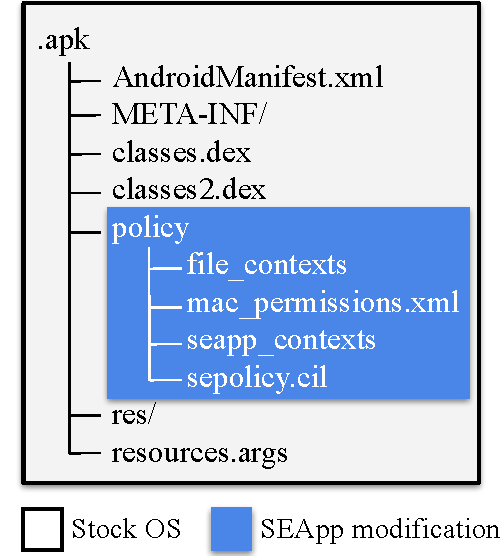
\includegraphics[width=0.4\textwidth]{chapters/seapp/figs/policy_folder}
	\caption{\seapp policy structure}
	\label{fig:seapp_policy_folder}
\end{figure}

\subsubsection{Processes}\label{subsub:seapp_process_control}

\seapp permits to assign a \sel domain to each process of the security
enhanced app.  To do this, the developer lists in the local
\seappcontexts a set of entries that determine the security context to
use for its processes.  For each entry, we restrict the list of valid
input selectors to {\tt user}, {\tt seinfo} and {\tt name}: {\tt user}
is a selector based upon the type of UID; {\tt seinfo} matches the app
seinfo tag contained in the local \macpermissions configuration file;
{\tt name} matches either a prefix or the whole process name.  The
conjunction of these selectors determines a class of processes, to
which the context specified by {\tt domain} is assigned.  To avoid
privilege escalation, the only permitted domains are the ones the app
defines within its policy module and \untrustedapp. As a process may
fall into multiple classes, the most selective one, with respect to
the input selector, is chosen.  An example of valid local
\seappcontexts entries is shown in Listing~\ref{seapp_lstseapp}, which
shows the assignment of the {\em unclassified} and {\em secret}
domains to the {\em :unclassified} and {\em :secret} processes,
respectively.

In Android, developers have to focus on components rather than
processes.  Normally, all components of an application run in a single
process.  However, it is possible to change this default behavior
setting the \texttt{android:process} attribute of the respective
component inside the \manifest, thus declaring what is usually called
a {\em remote} component.  Furthermore, with the specification of an
\texttt{android:process} consistent with the local \seappcontexts
configuration, we support the assignment of distinct domains to app
components.  To execute the component, the developer is only required
to create the proper \emph{Intent} object~\cite{seapp_intentsstart},
as she would have already done on stock Android for remote components.
The assignment to the process of the correct domain is handled by the
system.  This design choice allows us to support Android activities,
services, broadcast receivers and content providers, while avoiding
changes to the \textit{PackageParser}~\cite{seapp_packparse}, as there
are no modifications to the manifest schema.

\subsubsection{Files}\label{subsub:seapp_files_control}

The developer states the \sel security contexts of internal files in
the local \filecontexts.  Each of its entries presents three syntactic
elements, \texttt{pathname\textunderscore regexp},
\texttt{file\textunderscore type} and \texttt{security\textunderscore
  context}: \texttt{pathname\textunderscore re}- \newline {\tt gexp}
defines the directory the entry is referred to (it can be a specific
path or a regular expression); \texttt{file\textunderscore type}
describes the class of filesystem resource (i.e., directory, file,
etc.); \texttt{security\textunderscore context} is the security
context used to label the resource.  The admissible entries are those
confined to the app dedicated directory and using types defined by the
app policy module, with the exception of \appdatafile.  Due to the
regexp support, a path may suit more entries, in which case the most
specific one is used.  Examples of valid local \filecontexts entries
are shown in Listing~\ref{seapp_lstfile}: the first line describes the
default label for app files, second and third line respectively
specify the label for files in directories {\tt dir/unclassified} and
{\tt dir/secret}.

In \sel, the security context of a file is inherited from the parent
folder, even though \filecontexts might state otherwise.  Since, for
our approach, it is essential that files are labeled as expected by
the developer, we decided to enforce file relabeling at creation.
Therefore, a new native service has been added to the system (see
Section~\ref{sect:seapp_app_runtime}).  We then offer to the developer an
alternative implementation of class \texttt{java.io.File}, named
\texttt{android.os.File}, which sets file and directory context upon
its creation, transparently handling the call to our service.


\subsubsection{System services}\label{subsub:seapp_service_control}

To support any third-party app, the \untrustedapp domain grants to a
process the permissions to access all system services an app could
require in the \manifest.  As an example, in Android 11, the
\texttt{untrusted\textunderscore ap}- \newline {\tt p\textunderscore
  all.te} platform policy file~\cite{seapp_untrustedappte} permits to
a process labeled with {\tt untrusted}- \newline {\tt \textunderscore
  app} to access \texttt{audioserver}, \texttt{camera},
\texttt{location}, \texttt{mediaserver}, \texttt{nfc} services and
many more.

To prevent certain components of the app from holding the privilege to
bind to unnecessary system services, the developer defines a domain
with a subset of the \untrustedapp privileges (in the local \sepolicy
file), and then she ensures the components are executed in the process
labeled with it.  Listing~\ref{seapp_lstdomains} shows an example in
which the {\tt cameraserver} service is made accessible to the {\em
  secret} process.  \newline
\begin{lstlisting}[language=policyfile, caption=\seappcontexts
example, captionpos=b, label=seapp_lstseapp, numbersep=2pt,resetmargins=false]
 user=_app seinfo=cert_id domain=package_name.unclassified name=package.name:unclassified
 user=_app seinfo=cert_id domain=package_name.secret name=package.name:secret
\end{lstlisting}
%
\begin{lstlisting}[language=policyfile, caption=\filecontexts
example, captionpos=b, label=seapp_lstfile, numbersep=2pt,resetmargins=false]
 .*                u:object_r:app_data_file:s0
 dir/unclassified  u:object_r:package_name.unclassified_file:s0
 dir/secret        u:object_r:package_name.secret_file:s0
\end{lstlisting}
%
\begin{lstlisting}[language=policyfile, caption=Granting \texttt{cameraserver}
access to secret domain, captionpos=b, label=seapp_lstdomains, numbersep=2pt,resetmargins=false]
(block package_name
  (type secret)
  (call md_appdomain (secret))
  (typebounds untrusted_app secret)
  (allow secret cameraserver_service (service_manager (find)))...)
\end{lstlisting}

%%% Local Variables: 
%%% mode: latex
%%% TeX-master: "../../../main.tex"
%%% reftex-default-bibliography: "../../../bib/biblio.bib"
%%% End:
\section{Implementation}\label{sect:seapp_implementation}

In this section, we describe the main changes introduced in Android by
\seapp.  We first analyze the modifications required to manage policy
modules, both during device boot and at app installation.  We then
describe how the runtime support was realized.

\subsection{Policy compilation}\label{sect:seapp_syst_impl}

\subsubsection{Boot procedure}

Since the introduction of Project Treble \cite{seapp_treble}, policy
files are split among multiple partitions, one for each device
maintainer (i.e., platform, SoC vendor, ODM, and OEM).  This feature
facilitates updates to new versions of Android, separating the Android
OS Framework from the device-specific low-level software written by
the chip manufacturers.  Yet, each time a partition policy (i.e., a
segment) changes, an on-device compilation is required.

The \init process divides its operations in three
stages~\cite{seapp_initstages}: (i) {\em first stage} (early mount),
(ii) \sel setup, and (iii) {\em second stage} (init.rc).  The first
stage mounts the essential partitions (i.e., \dev, \proc, \sys and
\selinuxfsfull), alongside some other partitions specified as early
mounted (since Android 10 using an \fstab file in the first stage
ramdisk, in Android 9 and lower adding fstab entries using device tree
overlays).  Once the required partitions are mounted, \init enters the
SELinux setup.  As the name suggests, this is the stage where \init
loads the \sel policy.  As the \data partition, where policy modules
are stored, is not yet mounted, it is not yet possible to integrate
them with the policy of the system.  Then, as last operation of the
SELinux setup stage, \init re-executes itself to transition from the
initial \kernel domain to the \initdomain domain, entering the second
stage.  As the second stage starts, \init parses the \initrc files and
performs the builtin functions listed there, among them mounting the
\data partition.  Now, the policy modules are available, and we can
produce with \secilc~\cite{seapp_secilccom} (the \sel CIL compiler)
the binary policy consisting of the integration among the system
policy, the \seapp macros and the app policy modules.  To trigger the
build and reload of the policy, we implemented a new builtin function,
and modified the \initrc to call this function right after \data is
mounted.  The policy is considered immediately after the \data
partition is available and this ensures that the policy modules are
loaded far before an application starts, making the policy not
bypassable.

Even though most Android devices supporting Android 10 were released
with Treble support and, therefore, execute their \sel setup stage on
the \sepolicy fragments scattered among multiple partitions, \init
still supports the use of a legacy monolithic binary policy.  For
compatibility towards devices using a monolithic binary policy,
additional changes are required, as \seapp needs the system policy
written in CIL to be compiled alongside with app modules.  To this
end, we modified the Android build process to push the \sepolicy files
onto the device even for non-Treble devices.  New entries in the
device tree were added to make the policy segments available during
\init \sel setup stage \cite{seapp_early}.

As previously mentioned, we decided to store the policy modules in the
\data partition; even if this choice required us to adapt the boot
procedure of the device, it smoothly integrates \seapp with the current
Android design.  In fact, the \data partition is one of the few
writable partitions, it is dedicated to hold the APK the user
installs, as well as their dedicated data directories and, therefore,
it represents the best option to contain also the app policy modules.
Moreover, whenever a user performs a factory reset, Android
automatically wipes the \data partition, removing the customization
the user made to the device configuration, including the apps.  By
placing the app policy modules and the apps into the same partition, a
factory reset removes the policy modules as well.

\begin{figure}[h]
	\begin{center}
		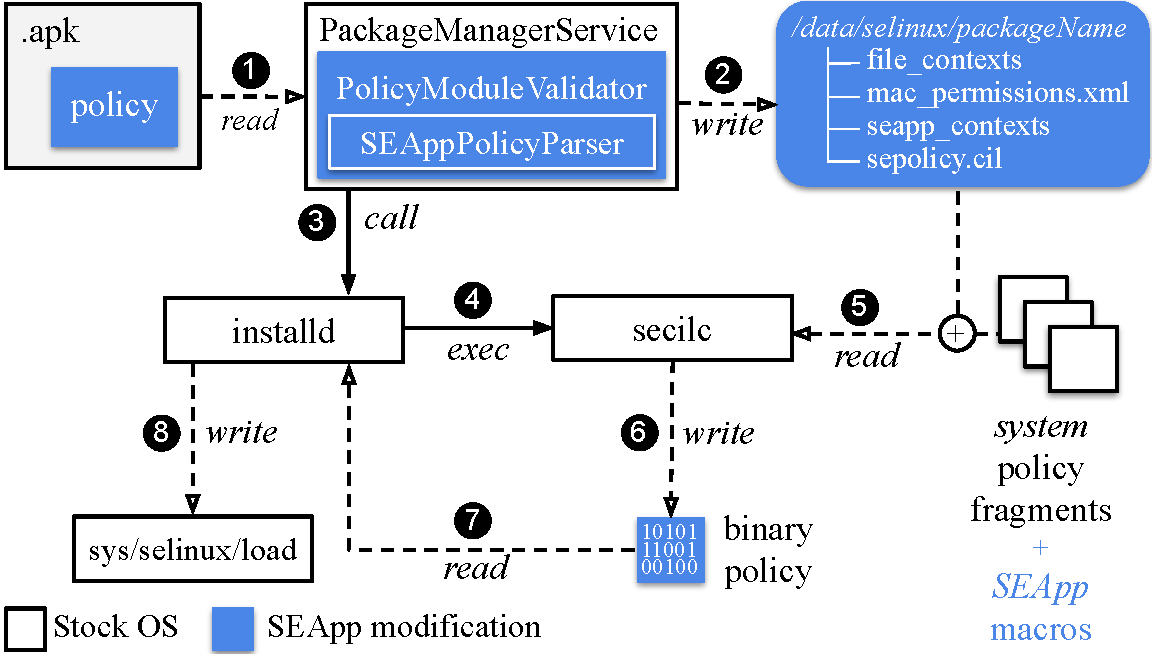
\includegraphics[width=0.8\columnwidth]{chapters/seapp/figs/app_installation}
	\end{center}
	\caption{\label{fig:seapp_install} Installation process}
\end{figure}

\subsubsection{App installation}

As introduced in Section~\ref{subsect:seapp_structure}, the developer
willing to define its own policy module is expected to load it in the
app package.  At app installation, the \pms~\cite{seapp_pmsserva}
inspects the APK to identify whether or not the current installation
involves a policy module, by looking for the \apkpolicydir directory
at the root of the archive.  When the app has a policy module attached
to it (see Figure~\ref{fig:seapp_install}), the \pms extracts it
(\blackcircle{1}) and uses our \textit{PolicyModuleValidator} to
verify the respect of all the constraints on \sepolicy (through the
{\em SEAppPolicyParser}, Section \ref{sect:seapp_lang}) and on the
configuration files (Section \ref{sect:seapp_config}).  In case of a
violation of the constraints, the app installation stops.  Otherwise,
the policy module is stored within \dataselinux, in a dedicated
directory identified by the package name (\blackcircle{2}).  Then, the
\pms invokes \installd~\cite{seapp_installdid} through the {\em
  Installer} to trigger the policy compilation with an exec call to
the \secilc program (\blackcircle{3}, \blackcircle{4}).  {\em Secilc}
reads the system \sepolicy fragments, the \seapp macros and the
\sepolicy fragments of the app policy modules in the \dataselinux
directory (\blackcircle{5}), and builds the binary policy
(\blackcircle{6}).  When the \secilc execution returns and no
compilation errors have been raised, the binary policy is then read by
\installd (\blackcircle{7}) and loaded with \loadpolicy, which writes
the \texttt{sys/selinux/load} file (\blackcircle{8}).

To load the policy files after \init, the implementation of SELinux in
Android has been slightly modified.  In particular, we modified the
policy loading function within \libselinux (function \loadpolicy), and
changed the system policy to allow \installd to load the app policy
module.

As for the policy configuration files, some changes were introduced to
load the application \filecontexts, \seappcontexts and
\macpermissions.  {\em SELinuxMMAC}~\cite{seapp_mmacsel}, i.e., the
class responsible for loading the appropriate {\tt mac\textunderscore
  pe}- \newline {\tt rmissions.xml} file and assigning \seinfo values
to apks, was modified to load the new \macpermissions specified within
the app policy module.  The loading of \filecontexts and
\seappcontexts was configured to treat system and app configuration
files apart.  So, \seapp-enhanced applications will load exclusively
their configuration files, whereas the loading of system's and other
apps' configuration files is not needed since their use is prohibited.
System services and daemons, instead, load the base system
configurations once, and then load the app policy module specific
configuration files as they are needed.  An example of this are
\zygote and \restorecon services, which need to retrieve at runtime
\seappcontexts and \filecontexts, respectively (see
Section~\ref{sect:seapp_app_runtime}).

Our implementation also supports the uninstallation of \seapp apps.  The
regular uninstallation process is extended with a step where the
global policy is recompiled, in order to remove the impact of old
modules on the overall binary policy.  With reference to application
updates, the native \installd runs with the necessary permission to
remove and apply new file types based on the content of the
\filecontexts.

\subsection{Runtime support}\label{sect:seapp_app_runtime}

In addition to the steps described above, other aspects have to be
considered in order to extend SELinux support at the application
layer.

\begin{figure}[h]
  \centering
  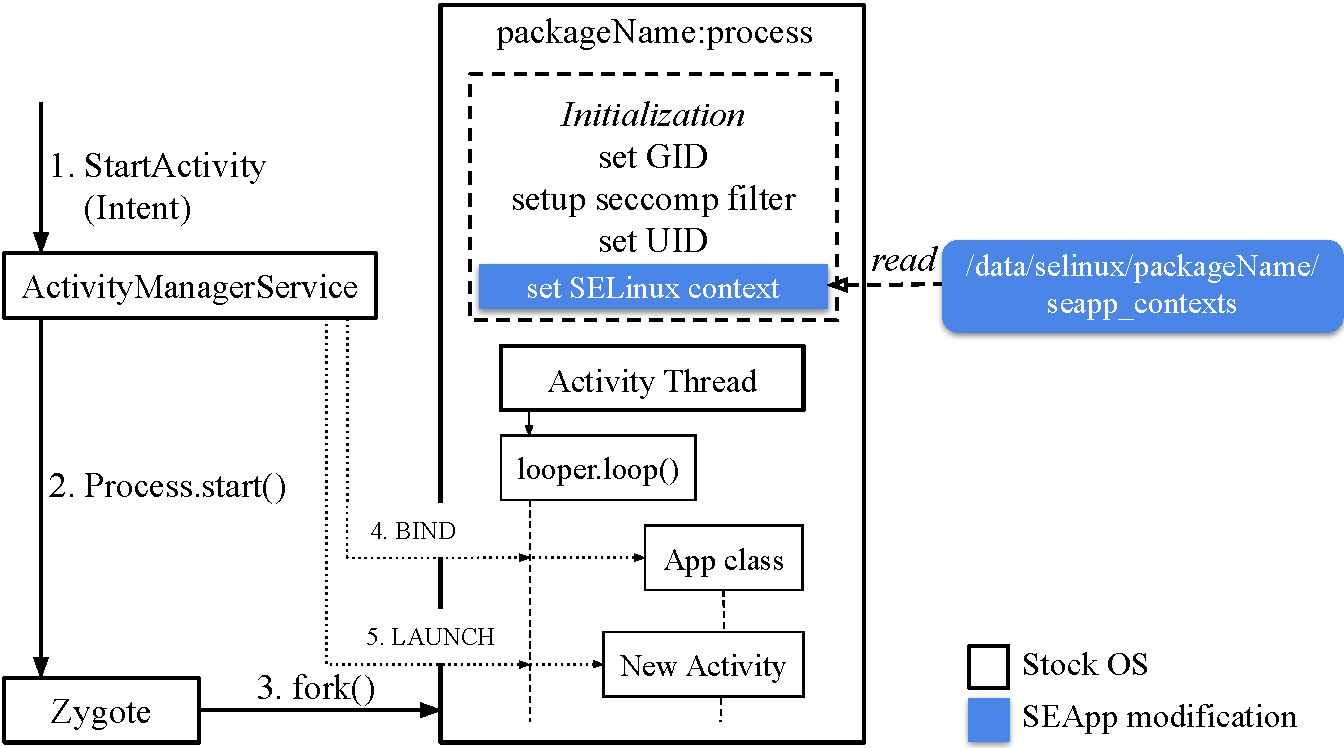
\includegraphics[width=0.8\columnwidth]{chapters/seapp/figs/app_launch}
  \caption{\label{fig:seapp_runtime} Application launch}
\end{figure}

\subsubsection{Processes}

Android application design is based on components.  Each of them lives
inside a process, and can be seen as an entry point through which the
system or the user can enter the app.

To activate a component, an asynchronous message called intent,
containing both the reference to the target component and parameters
needed for its execution, has to be created.  The intent is then
routed by the system to the {\em
  ActivityManagerService}~\cite{seapp_activitymanserv} via {\em Binder
  IPC}.  Before delivering the intent request to the target component,
the {\em ActivityManagerService} checks if the process in which the
target component should be executed is already running; if not, the
native service called \zygote~\cite{seapp_zygoterfi} is executed.  Its
role is to spawn and correctly setup the new application process.  To
achieve this, it first replicates itself by performing a fork, then,
using the input provided by the {\em ActivityManagerService} (namely,
package name, \seinfo, {\tt android:process}, etc.), it starts
configuring the process GID, the {\em seccomp} filter, the UID and
finally the \sel security context.  We adapted the final configuration
step, forcing \zygote to set the security context based on the
\seappcontexts located at {\tt \dataselinuxdir} (i.e., the one
provided by the developer for her app).  Process name is used to
assign the proper context to the process when it starts, before the
logic of the process kicks in.  In case the developer did not specify
a domain, then \zygote uses the system \seappcontexts as fallback.
After the correct labeling, the {\em ActivityManagerService} finishes
the configuration by binding the application class, launching the
component, and finally delivering the intent message.
Figure~\ref{fig:seapp_runtime} details the process.

This implementation design offers several benefits, including backward
compatibility, support for all components, and ease of use.
Indeed, a developer who wants to use our solution only has to
configure some files; changes in the application code are reduced to a
minimum, thus facilitating the introduction of SELinux in already
existing apps.

In our study we have also explored other design alternatives, in which
the developer could explicitly state a domain transition in the code,
wherever she needs it.  Although this category of solutions would give
the developers more control over domain transitions, it also has some
drawbacks.  First, the developer would be expected to enforce the
isolation among source and target domains managing the multi-threaded
scenario, and second, this design implies granting too many
permissions to the app (e.g., \dyntransition, \setcurrent and
read/write access to \selinuxfs).  Moreover, such solution would
introduce a new Android API, that would be quite delicate and, if not
used correctly, it might be difficult to control.

\begin{figure}[t]
  \begin{center}
    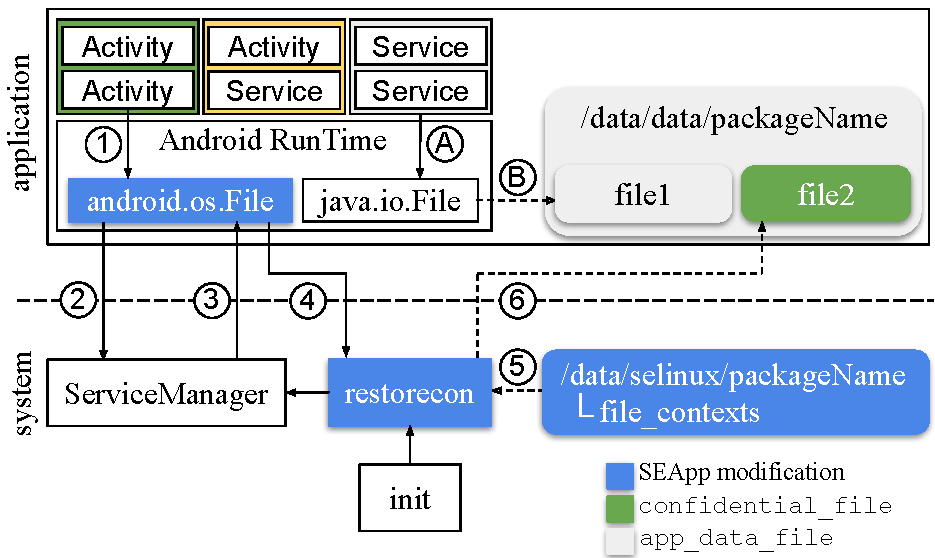
\includegraphics[width=0.8\columnwidth]{chapters/seapp/figs/restorecon_service}
  \end{center}
  \caption{\label{fig:seapp_restorecon} File relabeling}
\end{figure}


\subsubsection{Files}\label{sect:seapp_impl_files}

Android applications aiming to create a file can use the {\tt
  java.io.File} abstraction.  Each file creation request that is
generated is captured by the Android Runtime
(ART)~\cite{seapp_androruntime}, and then converted into the
appropriate syscall.  The result is the creation of the target file,
to which a security context inherited from the parent directory is
assigned (see flow \whitecircle{A}, \whitecircle{B} of
Figure~\ref{fig:seapp_restorecon}).  Since Android 9, the separation
between files of different apps is enforced at MAC level (a unique
context based on UID and \sel category is assigned); however, all the
files stored in the same app folder are labeled with the \appdatafile
type.

To make the most out of \sel, \seapp complements Android with the
implementation of a new service, which we called \restorecon (to
recall the \sel \restoreconc tool).  The \restorecon service is
spawned by {\em init} at boot, and works in its own \sel domain.  Its
role is to create and label files as specified by the developer in the
local \filecontexts.  To ease development, we implemented the new {\tt
  android.os.File} abstraction, which exposes an interface equal to
that of {\tt java.io.File}, and transparently handles the call to our
service.  Figure~\ref{fig:seapp_restorecon} details the new control
flow.  A component running in a \seapp-enhanced process (highlighted in
green in Figure~\ref{fig:seapp_restorecon}) invokes {\tt
  android.os.file}, and triggers a new file creation request
(\whitecircle{1}).  The new API first interacts with the {\em
  ServiceManager} (\whitecircle{2}) to get a handle of the \restorecon
service (\whitecircle{3}), then it interacts with the service using
the AIDL~\cite{seapp_aaidl} interface we defined for it, informing the
\restorecon of the target path (\whitecircle{4}).  The \restorecon
service verifies whether the caller is the legitimate owner of the
path, it reads the \filecontexts file located at \dataselinuxdir
(\whitecircle{5}), and finally it creates the target file enforcing
the correct labeling (\whitecircle{6}).

We also investigated three other implementation approaches: (i) change
of the default security context inheritance behavior for the {\em
  ext4} filesystem, (ii) execution of the \sel \restorecon operation
by the app, once the file is successfully created, and (iii) use of
\restorecond~\cite{seapp_restorecondd}.  The first option would change
the default behavior system-wide.  As it might cause compatibility
issues, we decided not to choose it.  The second option is not ideal
from a security standpoint, as it requires to grant the application
too many permissions (e.g., \relabelfrom, \relabelto, as well as
read/write access to \selinuxfs to check the validity of the \sel
context).  The third option refers to the use of \restorecond, a
system daemon that watches (inodes of) a configurable list of files
and checks that they are labeled as stated in the system
\filecontexts.  Although it may realize the control, \restorecond was
meant for a few system files, therefore its performance would hardly
scale, especially considering that \seapp needs to manage all files
created by \seapp-aware apps.  Another major issue is that this approach
is exposed to race conditions, because there is a delay between file
creation and its relabeling.

\begin{figure}[h]
	\centering
  \subfloat{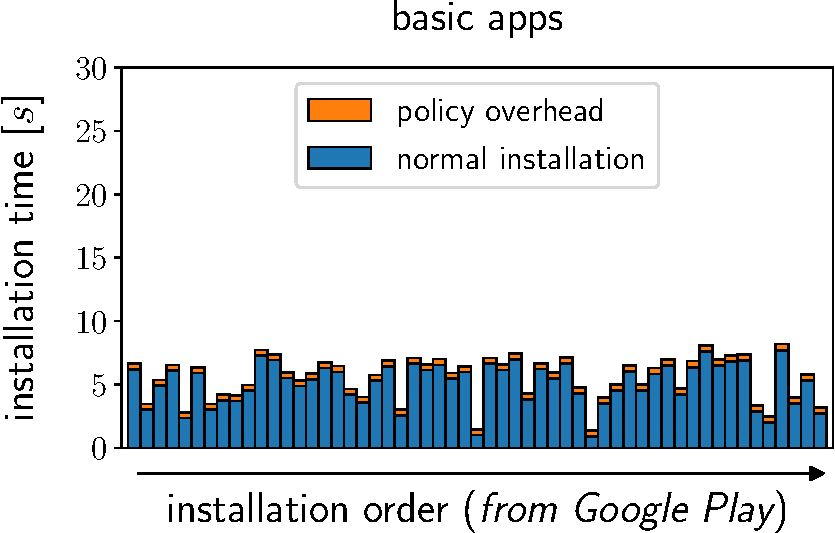
\includegraphics[width=185pt]{chapters/seapp/data/three_kinds_basic}}        
  \hfill
  \subfloat{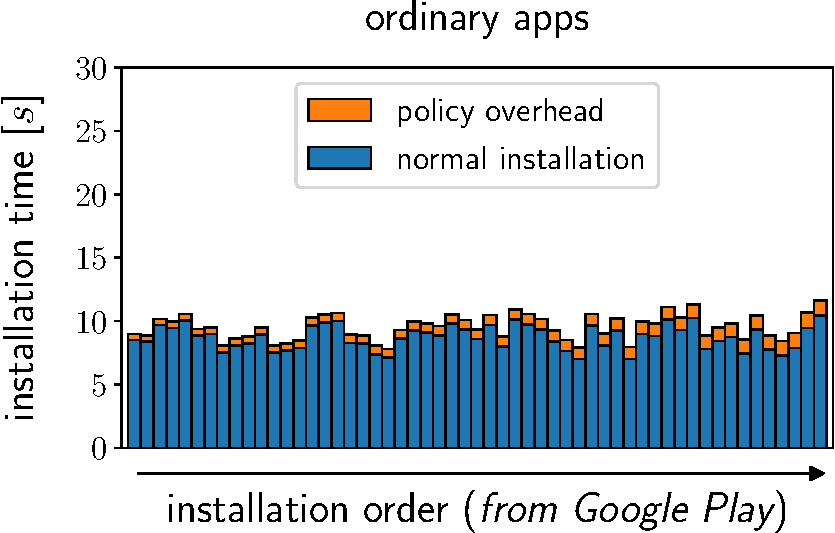
\includegraphics[width=185pt]{chapters/seapp/data/three_kinds_ordinary}}
  \\
  \subfloat{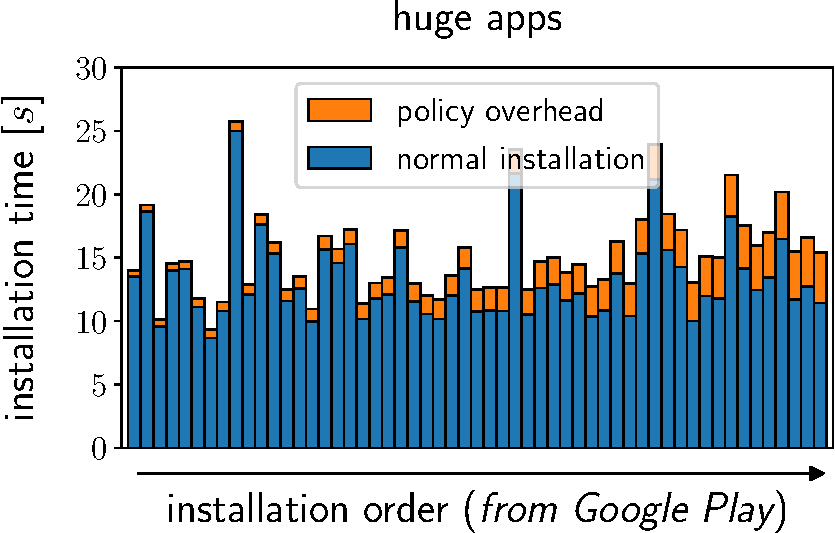
\includegraphics[width=185pt]{chapters/seapp/data/three_kinds_huge}}
	\caption{\label{fig:seapp_three_kinds} Installation time overhead for apps with different complexity}
\end{figure}      


%%% Local Variables: 
%%% mode: latex
%%% TeX-master: "../../../main.tex"
%%% reftex-default-bibliography: "../../../bib/biblio.bib"
%%% End:
\section{Experimental results}
\label{sect:seapp_performance}

We now present a performance evaluation of \seapp.  The experiments have
been conducted on both Android 9 and 10, each with Linux kernel v4.9.
However, all the measurements shown refer to Android 10 (release
android-10.0.0\textunderscore r41).  The device used to run the tests
is a Google Pixel 3 (\emph{blueline}), in which the four \emph{gold}
cores frequency was set to 2.8 GHz, while the four \emph{silver} ones
were disabled.  The change in CPU configuration has been performed to
reduce the variability of measures.  The confidence intervals provided
have an associated confidence level of 99\%.


\subsection{App installation}

The introduction of dedicated app policies implies further steps to be
executed at app installation time, as each \seapp module has to be
validated, compiled, and loaded.  To evaluate the impact on
performance, we wrote dedicated tests to stress the installation
procedure with multiple application samples.

To build representative samples of a typical consumer scenario, we
first downloaded the 150 most popular free apps from Google Play
(retrieved in October 2020)~\cite{seapp_topapps}.  The apps were
subsequently divided into three buckets: \emph{basic}, \emph{ordinary}
and \emph{huge} apps, according to the weighted normalized average of
the .apk size, the number of Android activities and the number of
services.  Based on the bucket, each app was equipped with one of the
following policy configurations: (i) \emph{basic}, 1 domain and 1 type
per policy module, (ii) \emph{ordinary}, 10 domains and 25 types, and
(iii) \emph{huge}, 20 domains and 100 types.  The rationale is that
larger apps can gain considerable benefit from the use of a large
policy.  The \emph{basic} configuration mimics how third-party apps
are currently handled, but with some key improvements, as it permits
to define the subset of services the domain can use, and it permits to
enforce app isolation, not only based on MAC category, but also
through the specification of its own type.  The \emph{ordinary} and
\emph{huge} policy configurations are meant to take full advantage of
intra-app isolation and flexibility via the definition of multiple
domains.
%
\begin{figure}[t]
	\centering
	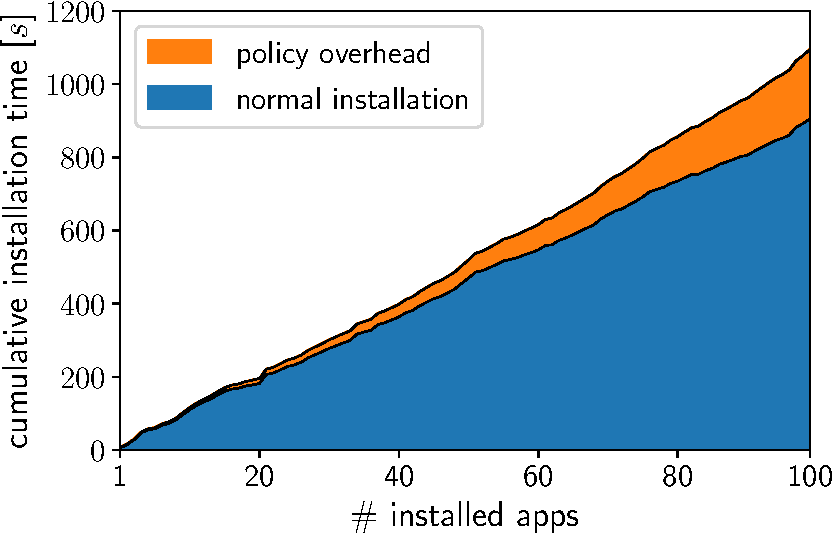
\includegraphics[width=0.7\columnwidth]{chapters/seapp/data/top100_cumulative}
	\caption[Cumulative install time overhead of the top 100 free apps
      with our policies]{
        \label{fig:seapp_benchmark100} Cumulative install time
        overhead when installing the top 100 free apps on Google Play
        Store with our policies
    }
\end{figure}
%
Each test was repeated five times, measuring the time each package
took to install.  The measurements were done with the *nix {\em date}
utility.

\noindent{\bf Test I.}
To measure the overhead caused by the presence of the policy module,
we performed on device installation of each of the previously
described app buckets (\emph{basic}, \emph{ordinary} and \emph{huge})
via Android Debug Bridge (adb)~\cite{seapp_adblink}.

The results of Test I are illustrated in
Figure~\ref{fig:seapp_three_kinds}.  In detail, it shows in blue
(i.e., the lower part of the bar) the time required by the system to
install the current package without the dedicated policy module, while
in orange (i.e., the top of the bar) the overhead caused by the
presence of the policy module.  The data report that a limited
overhead is associated with apps with \textit{huge} policies, at most
$3.59 \pm 0.04 s$, while \textit{basic} and \textit{ordinary} policy
configurations exhibit a negligible slowdown, never exceeding
$1.22 \pm 0.02 s$.

\noindent{\bf Test II.}
To evaluate the overall impact of \seapp in a typical consumer scenario,
we performed a test evaluating cumulative installations.  At first, we
repeated the installation of the top 100 apps on Google Play Store
with the same policy configuration as in Test I (see
Figure~\ref{fig:seapp_benchmark100}).  In this case, we measured an
overhead of $20.98 \pm 1,31\%$ on total installation time.

As explained in Section~\ref{sect:seapp_implementation}, each time a
new application is installed, all policy fragments stored in the
device have to be recompiled to produce the new binary policy.  The
installation time overhead then grows with the increase in the number
of installed policy modules.  To further analyze this aspect, we
repeated the installation of the top 100 free apps adding to all the
packages in three separate experiments the same \textit{basic},
\textit{ordinary}, and \textit{huge} policy configurations.  The
experimental results illustrated in
Figure~\ref{fig:seapp_install_time}, show that only the use of {\em
  huge} policy modules introduces a non-negligible overhead
($45.35 \pm 2.44\%$ on total installation time).  However, this policy
configuration simulates an edge case, as we do not expect to find 100
of them in a real scenario. To give a comparison, the {\em huge}
policy declares 100 types; {\tt public/file.te}, i.e., the file used
to define all the file types of the system, declares 314 types in
Android 10.

In Table~\ref{tab:seapp_policy} we report the sizes of the overall
policies for the three scenarios considered in this experiment.  We
report the number of MAC types, the number of produced AV rules, and
the overall size in KBytes of the binary policy.
%
\begin{table}[h!]
	\centering
        \small
	\begin{tabular}{|l|r|r|r|}
		\hline
		\textbf{policy} & \textbf{\#types} & \textbf{\#avrules} & \textbf{KB} \\ \hline
		system & 1536 & 29228 &  596 \\ \hline
		system + 100 basic & 1836 & 47028 &  867 \\ \hline
		system + 100 ordinary & 6036 & 213228 &  3512 \\ \hline
		system + 100 huge & 15536 & 417228 &  7064 \\ \hline
	\end{tabular}
	\caption{Policy size}
	\label{tab:seapp_policy}
\end{table}
%
\begin{figure}[t]
	\centering
	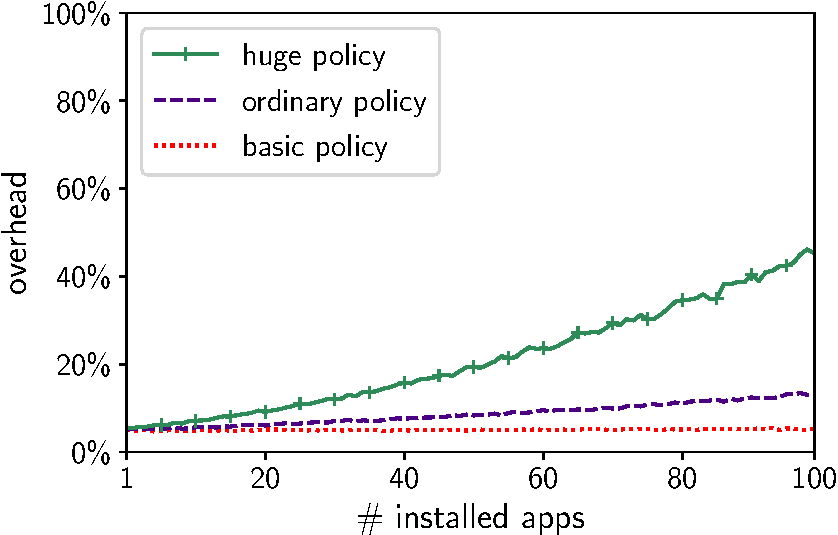
\includegraphics[width=0.7\columnwidth]{chapters/seapp/data/overheads}
	\caption{\label{fig:seapp_install_time} Install time overhead for the three policy sizes}
\end{figure}


\subsection{Runtime performance}

We now evaluate the runtime overhead for an app taking full advantage
of \seapp.  We focus on the creation of processes and files, as they are
the entities directly affected by the changes made in the
implementation.  The data shown refer to the creation time of each
resource.  The measurements have been acquired via
\textit{System.nanoTime} and have been repeated 100 times for each
test.  Also, all outliers diverging more than 3 standard deviations
from the mean have been suppressed.


\subsubsection{Processes}

As discussed in Section~\ref{sect:seapp_implementation}, in \seapp the
creation of a process is originated from the request of execution of
an Android component.  Thus, the slowdown occurs between the request
for the component and the execution of the method \textit{onCreate},
which is the time interval subject to measurement.  Our evaluation is
limited to activities and services, as these are the components most
used by developers.  Our analysis showed identical behavior for
broadcast receivers and content providers, the other two components
supporting the \process attribute in the manifest.

Separate test cases have been identified based on the type of process
that supports the component.  We refer to \emph{Local}, \emph{Remote},
\emph{Isolated} or \emph{\seapp} components when we run components
respectively in the current process, in another process, in another
process with the \isolatedapp domain (using the {\em isolatedprocess}
we described in Section~\ref{sect:seapp_int_comp_isolation}), or in a
package specific domain (declared in the app policy module).
Furthermore, we cover \emph{cold} and \emph{warm} start scenarios.
The {\em cold} start corresponds to the first time the application
brings up the component, and the {\em warm} start to the subsequent
times the app reuses a previously instantiated one.

\begin{table}[h]
  \centering
  \small
  \begin{tabular}{|l|c|c|c|c|c|c|c|c|} \cline{2-9}
    \multicolumn{1}{c|}{}&\multicolumn{4}{c|}{\textbf{Cold start
                           (ms)}}&\multicolumn{4}{c|}{\textbf{Warm start (ms)}} \\
    \cline{1-9}

    \multicolumn{1}{|c|}{\multirow{2}{*}{\textbf{\emph{Component}}}}&\multicolumn{2}{c|}{\textbf{\emph{Stock OS}}}&\multicolumn{2}{c|}{\textbf{\emph{\seapp}}}&\multicolumn{2}{c|}{\textbf{\emph{Stock OS}}}&\multicolumn{2}{c|}{\textbf{\emph{\seapp}}}  \\ \cline{2-9}

    \multicolumn{1}{|c|}{}  & $\mu$ & $\sigma$ & $\mu$ & $\sigma$ & $\mu$ & $\sigma$ & $\mu$ & $\sigma$   \\ \hline

        LocalActivity		& 39.102	& 1.094	& 38.689	& 0.980	& 21.052	& 6.046	& 18.685	& 5.001	\\ \cline{1-9}
        RemoteActivity	& 123.468	& 3.176	& 124.649	& 3.526	& 15.722	& 2.682	& 15.933	& 3.256	\\ \cline{1-9}
        \seapp Activity		& -			& -		& 127.356	& 3.542	& -			& -		& 15.188	& 2.394	\\ \cline{1-9}

    \hline \hline

        LocalService		& 19.164	& 1.444	& 18.835	& 1.392	& 1.399	& 0.208	& 1.328	& 0.208	\\ \cline{1-9}
        RemoteService		& 105.467	& 2.800	& 106.935	& 2.565	& 2.617	& 0.879	& 2.676	& 0.593	\\ \cline{1-9}
        IsolatedService	& 103.923	& 2.425	& 104.260	& 3.727	& -		& -		& -		& -		\\ \cline{1-9}
        \seapp Service		& -			& -		& 106.925	& 3.774	& -		& -		& 2.528	& 0.675 \\ \cline{1-9}
  \end{tabular}
  \caption{Cold and warm start performance for activities and
    services}
  \label{tab:seapp_start_2}
\end{table}

The results shown in Table~\ref{tab:seapp_start_2} demonstrate that
the performance of a stock version of the OS and \seapp are equivalent.
Also, we observe that apps willing to benefit of the intra-app
isolation feature get from the use of \seapp the same performance they
would get from the use of remote components.  Our approach also proves
to outperform the \textit{IsolatedService}, as the {\em
  isolatedprocess} option forces the creation of a new process every
time an {\em IsolatedService} that was previously {\em unBind}-ed is
activated.  This introduces a slowdown of $102 \pm 1 ms$ compared to
the {\em SEAppService} warm start, which instead benefits from the
system caching mechanism.

\subsubsection{Files}

Alongside the usual creation method, \seapp introduces in Android the
possibility of creating files with a security domain defined by the
app dedicated \filecontexts.  Table~\ref{tab:seapp_file_creation}
shows the time required to create a file, for each of the methods
discussed.  We observe no overhead on direct file creation, but the
overall execution time becomes larger due to the invocation, as
described in Section \ref{sect:seapp_app_runtime}, of the \restorecon
service, which requires approximately $374 \pm 30\mu s$.  This
overhead only occurs at file creation and every subsequent operation
on the file does not exhibit any performance degradation.

\begin{table}[h]
  \small \centering
  \begin{tabular}{|l|c|c|}
    \hline
    \multicolumn{3}{|c|}{\textbf{File creation}}  \\ \hline \hline
    \textbf{\textit{Test}} & \textbf{$\mu$ (\textmu s)} & \textbf{$\sigma$ (\textmu s)} \\ \hline
        Stock OS			&  57.077	&  5.174		\\ \hline
        \seapp				&  60.696	&  6.782		\\ \hline
        \seapp +                          & \multirow{2}{*}{431.472} & \multirow{2}{*}{109.494} \\
        \restorecon & & \\ \hline
  \end{tabular}
  \caption{File creation performance}
  \label{tab:seapp_file_creation}
\end{table}


%%% Local Variables: 
%%% mode: latex
%%% TeX-master: "../../../main.tex"
%%% reftex-default-bibliography: "../../../bib/biblio.bib"
%%% End:
\section{Related work}\label{sect:seapp_relwork}

In traditional desktop operating systems significant effort has been
spent in retrofitting legacy code for authorization policy enforcement
leveraging MAC.  An approach is to place reference monitor calls to
mediate sensitive access locations through the use of static and
dynamic analysis~\cite{seapp_jaeger_retro, seapp_jaeger_hook}.  An
evolution of this solution is the multi-layer reference
monitor~\cite{seapp_jaeger_web}, in which the MAC policy is enforced
at different levels (e.g., application, OS, Virtual Machine Manager).
Another approach is to identify integrity-violating permissions
through the use of information-flow analysis~\cite{seapp_jaeger_flow}.

Android's open source nature and popularity made it the target of
careful security investigations (e.g., \cite{seapp_sok_android,
  seapp_10.1007/978-3-319-20550-2_15, seapp_4768655,
  seapp_10.5555/2028067.2028088}) and several proposals aiming at
strengthen its security properties.  In the following we discuss the
ones that try to address app isolation and modularity, underlining the
key differences with our methodology.

Our approach presents similarities with {\em Secure Application
  INTeraction (Saint)} proposed by Ongtang et al. in
\cite{seapp_semantically_rich}, in which the authors also try to
address the issue of allowing developers to define policies that can
be verified at both installation time and runtime, to better specify
the permissions for each component of their app.  However, since the
paper has been published in 2010, {\em Saint} could not leverage
SEAndroid~\cite{seapp_seandroid}, which was introduced later, thus the
authors had to define their own Android security middleware, which
would not fit into the current Android
architecture~\cite{seapp_tapsm_m}.

{\em FlaskDroid}~\cite{seapp_flaskdroid} defines a versatile
middleware and kernel layer policy language.  It is based on Userspace
Object Managers (USOMs), which control access to services, intents and
data stored in Content Providers.  However, FlaskDroid does not focus
on intra-app compartmentalization, a central aspect in our proposal.

{\em ASM}~\cite{seapp_asm} and {\em ASF}~\cite{seapp_flaskdroid2}
promote the need for a programmable interface that could serve as a
flexible ecosystem for different security solutions. The generality of
these solutions, however, requires to introduce several changes to the
current Android security model.

{\em AppPolicyModules}~\cite{seapp_apm} is another proposal that
allows app developers to create dedicated policy modules. The authors
focus more on how apps could use SEAndroid to better protect their
resources from the system and from other apps, paying limited
attention to internal compartmentalization.

{\em DroidCap}~\cite{seapp_droidcap} is a recent contribution proposed
by Dawoud and Bugiel, in which the authors propose to replace
Android's UID-based ambient authority (DAC) with per-process Binder
object capabilities.  The proposal is interesting as it permits to
achieve security compartmentalization between different app
components. To introduce capability-based access control on files,
{\em DroidCap} had to integrate {\em Capsicum for
  Linux}~\cite{seapp_capsic} in Android. Overall, DroidCap is a nicely
engineered solution, which shares similar objectives with ours, and
the two could work in parallel as they do not interfere with each
other.  However, as our proposal relies on SELinux and SEAndroid,
which are already part of the Android security framework, our
architecture appears to be more aligned with the natural evolution of
the Android ecosystem.

{\em Boxify}~\cite{seapp_boxify} is a virtualization environment for
Android apps, which could be used to achieve a higher level of privacy
and better control over app permissions. The authors also describe how
their solution could be used to compartmentalize Ads libraries to
reduce the risk of sensible information leakage.  Yet, since the
virtualization environment acts as a mediator between the applications
and the system, it extends the set of trusted components the app has
to rely on.

{\em AFrame}~\cite{seapp_aframe} and {\em
  CompARTist}~\cite{seapp_10.1145/3133956.3134064} propose to
compartmentalize third-party libs from their host app using a separate
process with a dedicated UID. In {\em AFrame} the Android Manifest is
modified with the introduction of library ad-hoc permissions, while
{\em CompARTist} uses compile time app rewriting. Both proposals do
not extend the protection at the MAC level.

To summarize, the main differences that characterize our proposal are:
(i) we propose a natural extension of the role of SELinux to apps
leveraging what is already used to protect the system itself, thus
minimizing the impact on it, and (ii) we empower the developers while
limiting the amount of changes an application must undergo in order to
take advantage of our solution.

%%% Local Variables: 
%%% mode: latex
%%% TeX-master: "../../../main.tex"
%%% reftex-default-bibliography: "../../../bib/biblio.bib"
%%% End:
\section{Conclusions}\label{sect:seapp_conclusions}

This chapter proposed an extension to the current MAC solution (\sel)
already available in Android.  Developers can use \sel to define
domains that are internal to their apps, in such a way that it is
possible to leverage the modules that are already providing protection
to the system.  By mapping SELinux domains to activities and services,
developers can limit the impact that a vulnerability has on the app
processes and files.  We described in the chapter the changes that we
introduced into Android, and our experimental evaluation shows that
the overhead introduced by our proposal is compatible with the
additional security guarantees.

%%% Local Variables: 
%%% mode: latex
%%% TeX-master: "../../../main.tex"
%%% reftex-default-bibliography: "../../../bib/biblio.bib"


\section*{Availability}
The implementation source and artifacts produced for the evaluation of
our proposals are freely available at this URL:
\url{https://github.com/matthewrossi/seapp}

The work in this chapter was supported in part by the EC within the
H2020 Program under projects MOSAICrOWN, and by the 2015 Google
Faculty Research Award Program.


\chapter[Lightweight Cloud Application Sandboxing]{Lightweight Cloud Application \\ Sandboxing}
\label{chap:dmng}
\newcommand{\new}[1]{{\color{blue} #1}}
\newcommand{\fix}[1]{{\color{red} #1}}

\newcommand{\dmng}[0]{Dmng\xspace}
\newcommand{\ebpf}[0]{eBPF\xspace}

\colorlet{punct}{red!60!black}
\definecolor{background}{HTML}{EEEEEE}
\definecolor{delim}{RGB}{20,105,176}
\definecolor{types}{RGB}{255,0,0}
\definecolor{myBrickRed}{RGB}{203,65,84}

\lstset{
	xleftmargin=1.5em,
	basicstyle=\small\ttfamily,
	numbers=left,
	numberstyle=\scriptsize,
	stepnumber=1,
	numbersep=8pt,
	frame=lines,
	backgroundcolor=\color{background},
	captionpos=b,
}

\lstdefinelanguage{sh}{
	keywords=[1]{dmng},
	keywordstyle=[1]\color{blue},
	morecomment=[f][\color{myBrickRed}][0]{\#},
	extendedchars=true,
	showstringspaces=false,
	showspaces=false,
	breaklines=true,
	literate=
	*{:}{{{\color{punct}{:}}}}{1}
	{,}{{{\color{punct}{,}}}}{1}
	{\{}{{{\color{delim}{\{}}}}{1}
	{\}}{{{\color{delim}{\}}}}}{1}
	{[}{{{\color{delim}{[}}}}{1}
	{]}{{{\color{delim}{]}}}}{1}
	{<}{{{\color{delim}{<}}}}{1}
	{>}{{{\color{delim}{>}}}}{1},
}

\lstdefinelanguage{json}{
	xleftmargin=2em,
	basicstyle=\footnotesize\ttfamily\linespread{1.2},
	numbers=left,
	numberstyle=\scriptsize,
	stepnumber=1,
	numbersep=8pt,
	showstringspaces=false,
	breaklines=true,
	backgroundcolor=\color{background},
	literate=
	*{:}{{{\color{punct}{:}}}}{1}
	{,}{{{\color{punct}{,}}}}{1}
	{\{}{{{\color{delim}{\{}}}}{1}
	{\}}{{{\color{delim}{\}}}}}{1}
	{[}{{{\color{delim}{[}}}}{1}
	{]}{{{\color{delim}{]}}}}{1},
}

%%% Local Variables:
%%% mode: plain-tex
%%% TeX-master: t
%%% End:


\section{Introduction}
\label{dmng:sect:introduction}

With the research conducted on Android it soon became clear that,
while securing Android apps on the user device was very important,
it was as much important to secure the cloud applications those
applications interact with.
Cloud applications are often built of many components, each
implementing a specific set of business requirements. Components
naturally evolve, their requirements may change, and as the overall scale
of the application grows it can be challenging to ensure a high
security standard. Many factors contribute to making this objective
hard to achieve; the most common ones are: the presence of buggy
components, the reliance on potentially vulnerable native libraries
written with memory unsafe languages, and broad access to system
resources.

Several research works have investigated the scenario (e.g.,
\cite{staicu2021bilingual, binwrap,natisand, zimmermann-risks}). For
instance, Staicu et al.~\cite{staicu2021bilingual} explain the
security problems that arise when web applications interact with
native extensions. BinWrap~\cite{binwrap} and NatiSand~\cite{natisand}
analyze recent vulnerabilities and integrate new security
measures in the Node.js and Deno runtimes to improve isolation and
limit access to confidential resources. Lastly, 
Zimmermann et al.~\cite{zimmermann-risks} present an extensive study of third-party
dependencies, finding that large parts of the entire web ecosystem can
be impacted by security issues even when individual packages are
vulnerable or they include malicious code on purpose.

Recently, industry standards have also emerged to encourage
organizations to proactively include new security measures. A notable
example is the NIST SP 800-190~\cite{nist-sp800-190}, which focuses on
environments that adopt microservices, containers and Kubernetes. The
production environment is given particular attention, with the goal of
finding and stopping malicious threats in real time.  The directive
clearly indicates that there is a need for policies to defend against
vulnerabilities that could lead to disruptions, such as modification
of important files. The same regulation also provides instructions to
prevent the tampering of the file system, prompting that applications
and containers must be run with a set of permissions as minimal as
possible, namely following the {\em least privilege} principle.

Powered by the recent eBPF kernel technology, frameworks like
Tetragon~\cite{tetragon} and Falco~\cite{falco} have been proposed to
monitor cloud applications, identify unexpected security-relevant
events, and act on them (e.g., denying access). While effective, they
tend to introduce non-negligible overhead when fine-grained policy
rules are used~\cite{falco-overhead}.  We argue that the combined use
of classical operating system access control and sandboxing mechanisms
may lead to a more resource efficient solution to isolate application
components.  For instance, the recent Landlock LSM~\cite{landlock}
permits a process to restrict itself ensuring strong security
guarantees with minimum performance footprint.  Furthermore, the
integration of Landlock, or an equivalent security mechanism, in cloud
applications significantly mitigates the risk associated with the
exploitation of a vulnerability, as the amount of resources available
to a potential attacker is greatly reduced.

Unfortunately, to benefit from this protection developers must obtain
a policy that clearly states the resources an application component
must be granted access to, and the related permissions. This is far
from trivial in the case of complex applications. Indeed, the list of
resources can vary based on the production environment, or be subject
to changes when different inputs are provided. All these reasons hold
back the potential of sandboxing, and cloud applications may solely
rely on the coarse isolation provided by the virtual machine or the
container in which the application is executed.

\paragraph*{Our contribution}
In this chapter we propose a new approach to systematically integrate
fine-grained sandboxing in cloud applications that is aligned with the
current regulations and best practices. In detail, we provide an
intuitive, open-source solution to retrieve all the file system
resources required by an application component, to build and customize
least privilege policies. We then showcase how policies are used to
sandbox programs with Landlock, mitigating the impact of severe
CVEs. The approach we propose is flexible and does not depend on the
toolchain leveraged to build each application component. The
experiments showcase the minimal performance footprint at runtime, and
highlight the ability to monitor the application without affecting its
execution state.

%%% Local Variables:
%%% mode: latex
%%% TeX-master: "../main"
%%% End:

\section{Motivation}\label{sect:motivation}

This Section explains the threat model and the motivation.

\subsection{Threat model}\label{subsect:threat-model}

We assume that the code part of the cloud application (including
native code executed by it) is trusted and not malicious, but
potentially affected by vulnerabilities due to bugs.  In this
scenario, an attacker may leverage web interfaces or programmatic APIs
to send the application malicious payloads with the goal of exploiting
such vulnerabilities. This attack vector may leave the application
exposed to, e.g., arbitrary file read and write, file system
compromise, and execution of arbitrary programs; all of which can lead
to an inconsistent state of the application and its volumes. We aim at
the creation of fine-grained, component-specific policies that are
used by developers to gradually introduce sandboxing, mitigating the
impact of vulnerabilities. This approach is complementary to the use
of containers, as a compromised process running in a container can
still damage all the resources available to it.

\subsection{Dependency identification}

An important use case for cloud applications is represented by
services that handle media resources such as videos, photos, and
audio. These applications typically rely on an extensive set of
editing libraries and codecs to perform a number of operations like
crop, scale, introduction of effects, format conversion, and
compression. This software is usually available as dynamic libraries
that are loaded and executed depending on the type of operation to be
performed, on the input source, and on the hardware support
available. A solution able to automatically collect all the resources
used by a component for a set of test cases can significantly help the
developer detecting and isolating the dependencies of the application.

\subsection{Mitigation of bugs}

Open source libraries and programs are used extensively while
developing cloud applications. Examples include database drivers,
media processing libraries, and encoding utilities.  This software is
often trusted, but it may be subject to vulnerabilities as explained
in Section~\ref{subsect:threat-model}.  When vulnerable third-party
code is executed by the application, it can be targeted and
compromised by an attacker who sends malicious payloads, as described
in~\cite{sanddriller-staicu, cage4deno, npm-malicious-update}.
Popular cases are the Server-Side Request Forgery and Arbitrary File
Read vulnerabilities found in FFmpeg and exploited against
TikTok~\cite{ffmpeg-exploit-example}, and the Remote Command Execution
vulnerability found in ExifTool and exploited against
GitLab~\cite{exiftool-exploit-example}. Other examples include:
1)~CVE-2020-24020, CVE-2022-2566, CVE-2020-2499 associated with video
processing software, 2)~CVE-2022-1292, CVE-2022-2068, CVE-2022-2274
related to cryptographic software, and 3)~CVE-2021-4118,
CVE-2021-37678, CVE-2022-0845 targeting machine learning software.

With our approach we aim to support the progressive introduction of
fine-grained policies that are used to sandbox the application or any
of its components, making harder for an attacker to tamper the file
system, corrupt data, or exfiltrate sensitive information such as
private keys or database entries.

\subsection{Performance and usability}

Modern cloud applications are often deployed as Kubernetes Pod
instances and executed in one or more containers. Kubernetes provides
several tools to improve the security and isolation of Pods. Relevant
to this scenario are the support for RBAC policies and the
availability of restricted Seccomp profiles. RBAC policies by default
permit to define access of human users, however, they can also be used
to govern the behavior of software resources through {\em service
  accounts}. Unfortunately, these policies can only restrict access to
Kubernetes APIs, therefore they are not suitable for fine-grained
restriction of permissions at an application component level. The same
limitation is shared with Seccomp profiles, which can limit the kernel
interface available to the cloud application, but are only applied at
container level~\cite{k8s-seccomp} and cannot operate depending on the
specific requested resource~\cite{jia2023programmable}.

Recent solutions based on eBPF, like Tetragon and Falco, enable the
introduction of fine-grained policy rules to overcome the previous
limitations. To this end, they load into the kernel dedicated filters
which are run system-wide every time a security event like the opening of a file
or the execution of a program occurs. Based on the content of the
policy, and therefore the filters, these frameworks can grant or deny
a particular action, effectively restricting the privileges available
to a cloud application. However, as mentioned in Falco's
documentation~\cite{falco-overhead}, the main problem associated with
this approach is that performance overhead can have a large
variability. This is mainly due to the fact that filters are evaluated
every time a certain hook point (e.g., a syscall) is triggered, and
that many hooks may need to be controlled to enforce a given security
policy. Furthermore, these frameworks do not assist the developer in
the generation of application-specific policies.

With our proposal we aim at giving the developer a complementary
approach to secure applications and limit the file system resources
accessible to them.  Our idea is that the developer can benefit from
the advantages brought by technologies like Landlock (i.e., strong
security guarantees, low overhead), while at the same time rely on
eBPF-based technologies, but only to monitor a restricted subset of
important security events.

%%% Local Variables:
%%% mode: latex
%%% TeX-master: "../main"
%%% End:

\section{Approach overview}\label{sect:overview}

\begin{figure*}[t!]
  \centering
  \hspace*{-0.35em}
  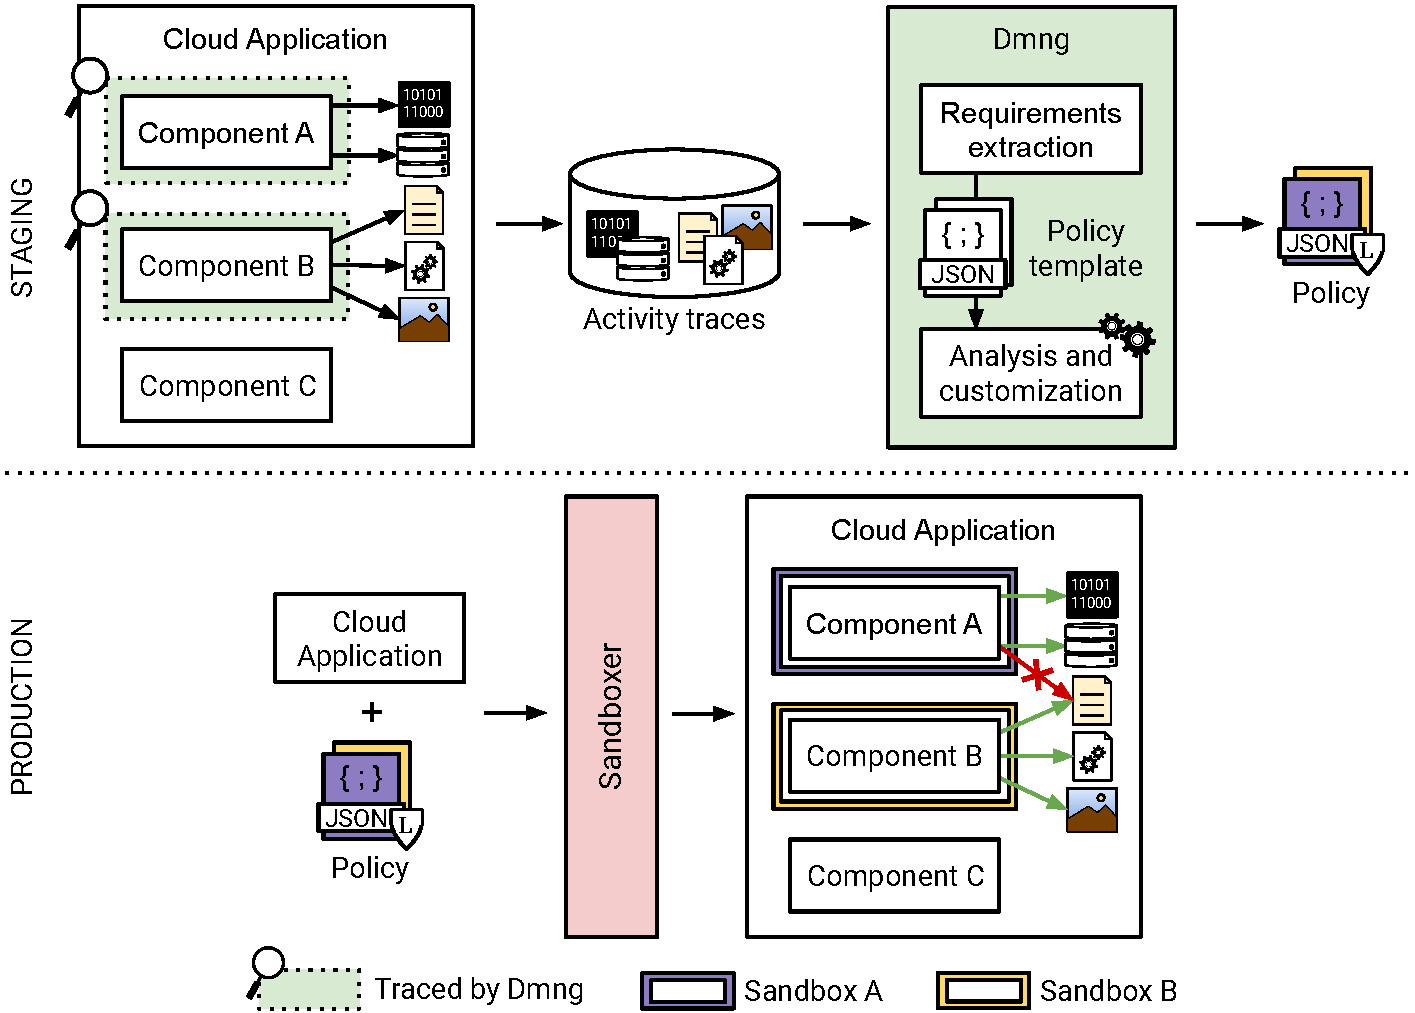
\includegraphics[width=1.01\linewidth]{chapters/dmng/fig/staging-prod.pdf}
  \caption[Overview of our approach]{Approach overview: 1)~\dmng uses
    probes to trace the application components A and B, 2)~activity
    traces are saved into a SQLite DB, 3)~requirements are extracted
    from the traces and used to build security policies, finally
    4)~policies are leveraged by the sandboxer to secure the
    application in production}
  \label{fig:overview}
\end{figure*}

Frequently, developers start building cloud applications from base
container images, which are subsequently customized and extended with
third-party software (e.g., web frameworks, database drivers, etc.).
Once the application has been developed, it is released to the staging
area, a replica of the production environment, not accessible from the
outside, where developers and cloud architects can test new features
so to detect design flaws and prevent unexpected errors to hit the
production environment.  The similarity to the production area makes
it the best candidate to generate accurate least privilege policies to
restrict the permissions available to the application.

To operate as intended, each application component requires access to
system resources like programs, scripts, dynamic libraries, shared
memory, and files. We simply call these resources {\em requirements}.
In order to collect them, we provide an intuitive open source tool
called \dmng that performs service instrumentation as shown in
Figure~\ref{fig:overview}.  In detail, the tool leverages ptrace and
eBPF to setup and activate temporary probes that register the actions
performed by an application component, making it possible to track
file-opening requests, reading and writing of data, use of shared
memory and execution of native code via subprocesses and shared
libraries. All these requests are automatically registered into a
database and subsequently used to generate policy templates. Together
with the file system path, each requirement is associated with
permissions. Compatibly with Unix-like systems, three permissions are
available: {\em read}, {\em write}, and {\em exec}. The policy
templates generated by \dmng can then be interactively modified by the
developer with the addition, modification or removal of policy
rules. After the changes are committed, the policy is serialized into
a JSON file and it is ready to be used to sandbox the application.

Sandboxing can be introduced with several technologies and frameworks;
given that we aim to restrict file system resources, we provide a
sandboxing utility based on Landlock that parses the set of
requirements needed by the application (i.e., path and permission
pairs) from the JSON policy file generated by \dmng, and it restricts
the permissions accordingly. We selected Landlock due to its
outstanding performance and stackability property.  Indeed, the use of
Landlock allows us to be compatible with systems that already rely on
other LSMs (e.g., AppArmor, SELinux).  We highlight that, whenever two
or more LSMs are available on the host, a single denial prevents the
access to a resource (i.e., deny takes precedence).

After the cloud application has been deployed to the production
environment it is important to ensure that services are running as
expected, there are no anomalies, and proactive measures are taken to
identify potential threats. By default, access to any file system
resource not listed in the policy is blocked by Landlock. However,
there may be cases in which the developer would like to generate
reports on the set of requested resources by the application. To
enable this, \dmng allows to temporarily observe and record the
activity traces generated by any application component without changes
to the application itself nor its execution state. These checks are
not bypassable, which is a considerable advantage compared to
alternative techniques that either rely on LD\textunderscore PRELOAD
or perform instrumentation through code dependency injection.

The following sections are organized as
follows. Section~\ref{sect:cloud-instrum} details the technologies
used to support policy generation and implement
monitoring. Section~\ref{dmng:sect:policy} clarifies the structure of the
policy. Section~\ref{sect:sandbox} describes sandboxing through
Landlock. Lastly, Section~\ref{dmng:sect:exp} showcases the mitigation
capabilities and investigates the performance overhead.


%%% Local Variables:
%%% mode: latex
%%% TeX-master: "../main"
%%% End:

\section{Cloud application instrumentation}\label{sect:cloud-instrum}

Our solution implements two methods to collect the requirements and
generate the policy. The first is uses ptrace and is based on syscall
argument inspection, the second leverages eBPF, which dynamically
extends the kernel attaching dedicated probes on relevant
\mbox{in-kernel} file system-related events. Both the approaches are
used to instrument the application, however, using ptrace
significantly affects performance and thus is meant to be used only
during staging. On the other hand, eBPF has lighter impact on
performance, hence it can be used also in production.

\subsection{Ptrace-based instrumentation}\label{sect:deep-instr}

Ptrace is a functionality implemented by the kernel aimed at debuggers
and code analysis tools that permits a process, called the {\em
  tracer}, to control and observe the activity performed by another
process, the {\em tracee}. In our implementation, \dmng acts as the
tracer for any application component. To this end, it prepares a
parent and a child process as shown in Figure~\ref{fig:ptrace}, and
then uses the ptrace system call to instruct the kernel that the child
will be traced by the parent (through the PTRACE\textunderscore
  TRACEME request). After this step is completed, \dmng injects into
the child process the component to be run, and then starts it.  While
being traced, every time an event occurs, the tracee is stopped by the
kernel and a notification is sent to the tracer, which has the
possibility to inspect and perform changes before the execution of the
tracee is resumed.  \dmng leverages ptrace to capture all file
system-related syscalls, effectively monitoring the requests issued to
the kernel by the component. The syscalls and their arguments are
recorded by the tracer and saved to the SQLite database mentioned in
Section~\ref{sect:overview}. The set of monitored syscalls includes
interfaces such as open, openat, creat, execve, link, linkat, mkdir,
and the related permission flags (e.g., O\textunderscore APPEND,
O\textunderscore CREAT, O\textunderscore RDONLY). It is
important to point out that \dmng automatically captures and monitors
the possible children spawned by the tracee, and it is also capable to
identify the set of dynamic libraries they depend upon.
% Moreover, when the developer releases the application
% component as a separate library, \dmng also permits to collect the
% dynamic libraries it depends on. To this end it uses {\em ldd}, which
% extracts transient dynamic libraries without running the entire
% application.
% \quest{I've commented this out because it comes out of the blue, and
% without a proper explanation raises more questions than answers}

\begin{figure}[t!]
  \centering
  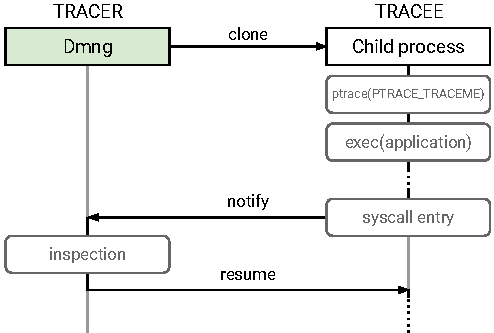
\includegraphics[width=0.6\columnwidth]{chapters/dmng/fig/ptrace_overview.pdf}
  \caption[Architecture of the ptrace-based instrumentation]{\dmng acts as a
    tracer for the application, inspecting the arguments of every
    syscall}
  \label{fig:ptrace}
\end{figure}

When the developer wants to stop the tracing process, \dmng detaches
itself from the tracing of the child process with the
PTRACE\textunderscore DETACH request and it terminates the child
process by sending a SIGKILL signal.

\subsection{eBPF-based intrumentation}\label{sect:cont-monit}

Similarly to other recent security and observability frameworks, like
Cilium~\cite{cilium-repo}, and Tetragon~\cite{tetragon}, \dmng relies
on the eBPF technology to implement continuous monitoring. The eBPF
subsytem allows to change at runtime the behavior of the kernel
without changing its implementation nor adding new modules. Briefly,
it permits to do so by loading compact programs within the kernel,
which are evaluated (without preemption) by a virtual machine-like
component every time a certain hook point is reached. There are many
types of hook within the kernel, examples are network events,
tracepoints, and LSM functions. To store data persistently between
different eBPF program invocations and to share data between kernel
and user space, data structures called {\em maps} are used. They
provide abstractions such as arrays and hashmaps. It is important to
mention that eBPF programs must be safe to run within the kernel and
must not introduce bugs. To ensure these conditions are met, the eBPF
susbsystem automatically performs the two stages of Program
Verification and Just-In-Time Compilation at load time; only if both
terminate without exceptions then the loading of the program is successful.

\begin{figure}[t!]
  \centering
  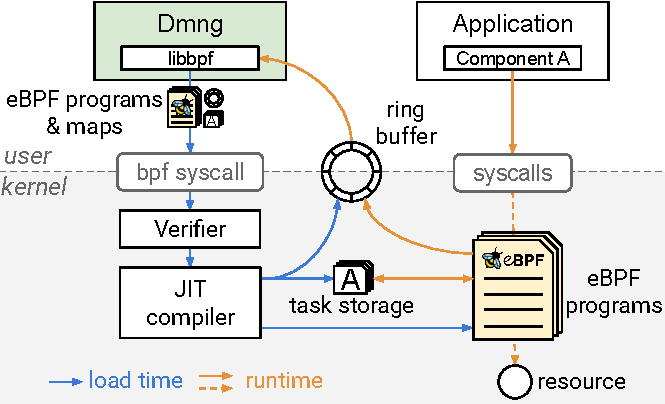
\includegraphics[width=0.7\columnwidth]{chapters/dmng/fig/ebpf_overview.pdf}
  \caption[Architecture of the eBPF-based instrumentation]{\dmng uses
    libbpf to load the eBPF tracing programs and maps, then it polls
    data from the shared ring buffer}
  \label{fig:ebpf}
\end{figure}

\dmng activates eBPF-based tracing on a given application component
using its thread identifier. To this end, it leverages the {\em
  libbpf}~\cite{libbpf-doc} frontend to load into the kernel the eBPF
programs and maps needed to perform tracing, and then starts
collecting data. The process is shown in Figure~\ref{fig:ebpf}.  The
set of eBPF programs comprises of: 1)~dedicated programs to trace the
application component lifetime, and 2)~programs to monitor the file
system-related events generated by the component. The former group of
programs ensure that monitoring extends to tasks spawned through the
clone system call by the component. Hence, they are attached to the
{\em sched\textunderscore process\textunderscore fork} and {\em
  sched\textunderscore process\textunderscore exit} kernel
tracepoints. Instead, the programs that record file system-related
events are attached to hooks reported in
Table~\ref{table-fs-hooks}. Whenever one of these hooks is triggered,
the attached program writes the requirement path and the related
permission to a ring buffer shared with the \dmng user space
process. This permits \dmng to poll data regularly, and then to save it
in the already mentioned SQLite database
(Section~\ref{sect:overview}).

We highlight that the collection of data using this method has minimal
invasiveness: no changes must be introduced in the code of the
application, nor it is necessary to restart it to setup the process.
Indeed, when the developer wants to stop tracing, the eBPF programs
and maps loaded by \dmng are automatically removed, leaving the system
unmodified.

\begin{table}[t]
  \centering
  \small
  \caption{List of file system traced hook points}
  \label{table-fs-hooks}
  \begin{tabular}{ l }
    \toprule
    \multicolumn{1}{ c }{\bf Hook name}\\
    \midrule
    {\tt fentry/security\textunderscore file\textunderscore fcntl}                        \\
    {\tt fentry/security\textunderscore file\textunderscore ioctl}                        \\
    {\tt fentry/security\textunderscore file\textunderscore lock}                         \\
    {\tt fentry/security\textunderscore file\textunderscore mprotect}                     \\
    {\tt fentry/security\textunderscore file\textunderscore open}                         \\
    {\tt fentry/security\textunderscore file\textunderscore receive}                      \\
    {\tt fentry/security\textunderscore file\textunderscore set\textunderscore owner}     \\
    {\tt fentry/security\textunderscore inode\textunderscore getattr}                     \\         
    {\tt fentry/security\textunderscore path\textunderscore chmod}                        \\
    {\tt fentry/security\textunderscore path\textunderscore chown}                        \\
    {\tt fentry/security\textunderscore path\textunderscore chroot}                       \\
    {\tt fentry/security\textunderscore path\textunderscore link}                         \\            
    {\tt fentry/security\textunderscore path\textunderscore mkdir}                        \\    
    {\tt fentry/security\textunderscore path\textunderscore mknod}                        \\
    {\tt fentry/security\textunderscore path\textunderscore rename}                       \\
    {\tt fentry/security\textunderscore path\textunderscore rmdir}                        \\    
    {\tt fentry/security\textunderscore path\textunderscore symlink}                      \\
    {\tt fentry/security\textunderscore path\textunderscore truncate}                     \\
    {\tt fentry/security\textunderscore path\textunderscore unlink}                       \\
    {\tt lsm/bprm\textunderscore check\textunderscore security}                           \\
    {\tt lsm/mmap\textunderscore file}                                                    \\
    \bottomrule
  \end{tabular}
\end{table}


%%% Local Variables:
%%% mode: latex
%%% TeX-master: "../main"
%%% End:

\section{Policy}\label{sect:policy}

In this section we present the structure of the policy, explaining how
it can be customized. We also discuss aspects such as coverage and
effectiveness.

\paragraph*{Policy structure} The policy obtained from \dmng is a JSON
file structured as a list of objects as shown in
Listing~\ref{lst:policy_file}. For each of them, a field {\em
  policy\textunderscore name} identifies the application component the
policy applies to, while the sections {\em read}, {\em write} and {\em
  exec} are used to configure the related permissions. The structure
of the policy is flexible, and for each object only the field {\em
  policy\textunderscore name} is required. Since the policy implements
a \mbox{{\em default-deny}} model, an object that does not list any
section in its body has no runtime permission, hence the corresponding
component cannot access any file system
resource. Listing~\ref{lst:policy_file} shows an example in which a
component called {\em filter} is granted execution access to the Awk
program (together with its shared libraries) to process the
\mbox{read-only} {\em users.csv} dataset.

\paragraph*{Policy customization} \dmng provides a CLI interface that
work simultaneously with multiple data sources to produce the list of
requirements. By default, it implements the logic to automatically
merge the requirements collected with ptrace and the eBPF
programs. Moreover, it permits to customize the policy interactively,
adding, changing and removing requirements. For instance, it allows to
delete requirements based on the permission mask (e.g., {\tt
  r\textunderscore x}, {\tt r--}), or change the permission associated
with all the requirements that match a given path regex (e.g., {\tt
  /usr/bin/libnet.*}).  \newline A useful feature implemented by \dmng
is {\em permission pruning}. This function takes advantage of the
structure of the Directory Tree~\cite{hier} to help the developer
lower the number of requirements in the policy by reducing the
granularity of permissions. The reduction in granularity is based on a
{\em pruning goal} set by the developer that represents the desirable
maximum number of policy rules associated with an application
component. To implement this feature, \dmng first uses the policy
template to build a trie (or prefix tree), then starts pruning its
branches iteratively following a best effort approach, until the
pruning goal is achieved.  The rationale is that there are areas of
the file system in which fine granularity brings strong security
guarantees (e.g., {\tt /lib}), but there are also many other areas
where fewer rules make the policy more concise without affecting
security (e.g., {\tt /share}). So, it is important to consider
contextual information about the current prefix path to guide the
pruning process.  Moreover, we want to comply with the {\em write xor
  execute} memory protection policy whereby every file may be either
writable or executable, but not both. Thus, limiting the propagation
of potentially insecure configurations (e.g., no dynamic library
stored in {\tt /lib} must be writable and executable by the
application).  After the pruing process terminates, the changes to the
template are audited by the developer, and can be committed or
discarded.


\begin{lstlisting}[
  caption=Example of JSON file with single policy,
  float=tp,
  floatplacement=tbp,
  language=json,
  label=lst:policy_file,
  frame=none,
  aboveskip=-0.3em,
]
{
  "policies": [{
      "policy_name": "filter",
      "read": [
        "/lib/x86_64-linux-gnu/libsigsegv.so.2",
        "/lib/x86_64-linux-gnu/libreadline.so.8",
        "/lib/x86_64-linux-gnu/libmpfr.so.6",
        "/lib/x86_64-linux-gnu/libgmp.so.10",
        "/lib/x86_64-linux-gnu/libm.so.6",
        "/lib/x86_64-linux-gnu/libc.so.6",
        "/lib/x86_64-linux-gnu/libtinfo.so.6"',
        "/lib64/ld-linux-x86-64.so.2",
        "/usr/bin/awk",
        "users.csv"
      ],
      "exec": [
        "/lib/x86_64-linux-gnu/libsigsegv.so.2",
        "/lib/x86_64-linux-gnu/libreadline.so.8",
        "/lib/x86_64-linux-gnu/libmpfr.so.6",
        "/lib/x86_64-linux-gnu/libgmp.so.10",
        "/lib/x86_64-linux-gnu/libm.so.6",
        "/lib/x86_64-linux-gnu/libc.so.6",
        "/lib/x86_64-linux-gnu/libtinfo.so.6"',
        "/lib64/ld-linux-x86-64.so.2",
        "/usr/bin/awk"
      ]
  }]
}
\end{lstlisting}

\paragraph*{Coverage and effectiveness}

To generate the policy templates, \dmng registers the activity
performed by the application while a set of test cases is
executed. This approach is similar to the one proposed by the Slim
toolkit~\cite{slimtoolkit} to identify the dependencies of a container
and minify its image, and to the one followed by the Google Sandbox2
utility~\cite{sandbox2} to retrieve the requirements of programs
distributed as ELF files. However, test-based policy generation can be
subject to coverage issues if the set of test cases is not
exhaustive. Another aspect worth mentioning is that applications
poorly structured may benefit less from the isolation properties
provided by sandboxing. Indeed, on a traditional Unix operating
system, components executed within the same thread will inevitably
share the same policy. Since \dmng supports the sandboxing of
components with a per-thread policy, we recommend to leverage this
function and execute potentially vulnerable components in dedicated
compartments.

%%% Local Variables:
%%% mode: latex
%%% TeX-master: "../main"
%%% End:

\section{Application sandboxing}\label{sect:sandbox}

\begin{figure}[t!]
  \centering
  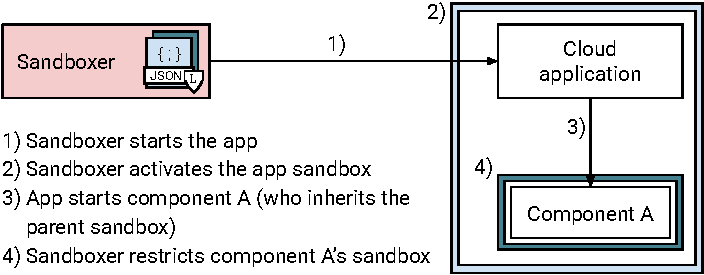
\includegraphics[width=0.8\columnwidth]{chapters/dmng/fig/landlock_overview.pdf}
  \caption{Landlock sandbox setup and inheritance}
  \label{fig:landlock}
\end{figure}

In this work we implement the sandbox leveraging Landlock, an
unprivileged sandboxing mechanism officially merged into the Linux
kernel in 2021 (version 5.13), with the goal of mitigating the
security impact of bugs and unintended or malicious behavior in
user-space application. The main reasons why Landlock was preferred to
alternative sandboxing solutions such as Google
Sandbox2~\cite{sandbox2} are: 1) it does not rely on a proxy to
implement the restrictions, hence it ensures low overhead at runtime,
and 2) it is directly implemented within the kernel, thus it provides
strong security guarantees. This section clarifies how policies are
enforced with Landlock. Furthermore, it explains how {\tt rwx} policy
rules are translated into the Landlock permission model, and how
restrictions are inherited by new components dynamically spawned at
runtime.

The sandboxer is an extension of \dmng written in Rust that receives
the JSON policy as input and modifies the application start procedure
setting the permissions available to components before they are
executed. The first task performed by the sandboxer is then to
translate the {\tt rwx} policy rules into the action-based permission
model implemented by Landlock. In detail, Landlock groups permissions
into {\em rulesets}, which collect the {\em actions} (e.g.,
FS\textunderscore EXECUTE, FS\textunderscore READ\textunderscore FILE)
permitted on each {\em object} (e.g., file, directory). The sandboxer
separates the available actions to match the {\tt rwx} categories, and
then leverages the {\em landlock\textunderscore create\textunderscore
  ruleset()} and {\em landlock\textunderscore add\textunderscore
  rule()} interfaces to populate the rulesets accordingly. To activate
the restrictions, a call to {\em landlock\textunderscore
  restrict\textunderscore self()} is perfomed. The process is
illustrated in Figure~\ref{fig:landlock}.

An important property defined by Landlock is {\em policy inheritance}.
Whenever a new component is dynamically spawned by the application in
a child process, it automatically inherits the restrictions set on the
parent. Moreover, after a ruleset has been activated, no new
permissions can be granted to a component, as the ruleset can only be
further restricted. Figure~\ref{fig:landlock} shows the policy
inheritance process for a generic application. The figure also shows
how the inherited ruleset is further narrowed with a subsequent call
to {\em landlock\textunderscore restrict\textunderscore self()} by the
component.



%%% Local Variables:
%%% mode: latex
%%% TeX-master: "../main"
%%% End:

\section{Experiments}\label{dmng:sect:exp}

This section presents our experimental evaluation. In the first part
(Section~\ref{dmng:sect:exp-mitig}), we show the benefits coming from the
introduction of sandboxing in cloud applications. In detail, we
reproduce a sample of CVEs affecting open source software, and
showcase how the sandbox mitigates the exploits. In the second part
(Section~\ref{dmng:sect:exp-perf}), we analyze the performance
overhead. Specifically, we implement an application that performs
various operations on media resources, and then evaluate the
degradation of latency when sandboxing and eBPF-based monitoring are
activated. The tests have been executed on a workstation with Arch
Linux, kernel version 6.4, an AMD Ryzen 5 7600X CPU, 32 GB RAM, and 1
TB SSD.

\subsection{Mitigation of vulnerabilities}\label{dmng:sect:exp-mitig}

To demonstrate the importance of the introduction of sandboxing, we
selected the sample of high severity vulnerabilities reported in
Table~\ref{table:cve}. These vulnerabilities affect software
extensively used in cloud application development such as FFmpeg,
ImageMagick, OpenSSL and Exiftool. For each of them, we installed on
the system a vulnerable version of the program or library, and then
verified it was exploitable using public Proof of Concepts when the
input is sent through programmatic APIs or web
interfaces. Subsequently, we leveraged \dmng to generate least
privilege policies as explained in
Section~\ref{sect:cloud-instrum}. Finally, we repeated the execution
of the previous tests starting each vulnerable component with our
sandboxer. When benign input was submitted to the application, we were
successfully able to conduct the tests without loss of
functionality. When instead malicious input was used, Landlock
correctly blocked the exploit, limiting access to only resources
listed in the policy. We highlight that, in general, similar
protections extend to a broader set of CVEs.


\begin{table}[!t]
  \footnotesize
  \caption{\label{table:cve} Sample of CVEs reproduced in our evaluation}
  \setlength{\tabcolsep}{0.2cm}
  \begin{tabularx}{\columnwidth}{ l l l >{\raggedright\arraybackslash}X}
    \toprule
    {\bf CVE} & {\bf Software} & {\bf Version} & {\bf Description}\\
    \toprule
    CVE-2016-1897  & \multirow{2}{*}{FFmpeg} & \multirow{2}{*}{v2.x} & A crafted AVI video is used to read arbitrary \\
    CVE-2016-1898  & & & files \\
    \midrule
    CVE-2020-29599  & ImageMagick  & v7.0.10-36  & A bug in the PDF codec enables arbitrary code execution \\
    \midrule
    CVE-2022-1292  & OpenSSL  & v3.0.2 & Improper sanitisation allows command injection \\
    \midrule
    CVE-2021-22204   & ExifTool        &  v12.23 & Improper neutralization of user data in the DjVu file format is used to run arbitrary executables \\
    \bottomrule
  \end{tabularx}
\end{table}

\subsection{Overhead}\label{dmng:sect:exp-perf}

As mentioned in Section~\ref{sect:motivation}, an important use case
for cloud applications is represented by services that handle media
resources such as videos, photos and audio. Therefore, to evaluate the
overhead associated with our approach we implemented a Rust
application that, upon receiving a request, leverages third-party
software to apply several transformations on a media resource. Our
goal is to measure the latency, or rather the time taken by the
application to perform a given operation. Three test configurations
are used: 1)~no sandboxing is applied, hence no protection,
2)~sandboxing is enabled leveraging our Landlock-based sandboxer, and
3)~sandboxing is enabled plus eBPF-based continuous monitoring
provided by \dmng is activated. Each operation is repeated 1000 times,
and the measures are reported with 95\% confidence intervals. Moreover, we focus on the
server-side execution time, hence we do not consider the delay
introduced by the network, which may make harder to visualize latency
degradation for short-lived operations.

\begin{figure*}[t!]
  \begin{subfigure}[b]{0.5\linewidth}
    \centering
    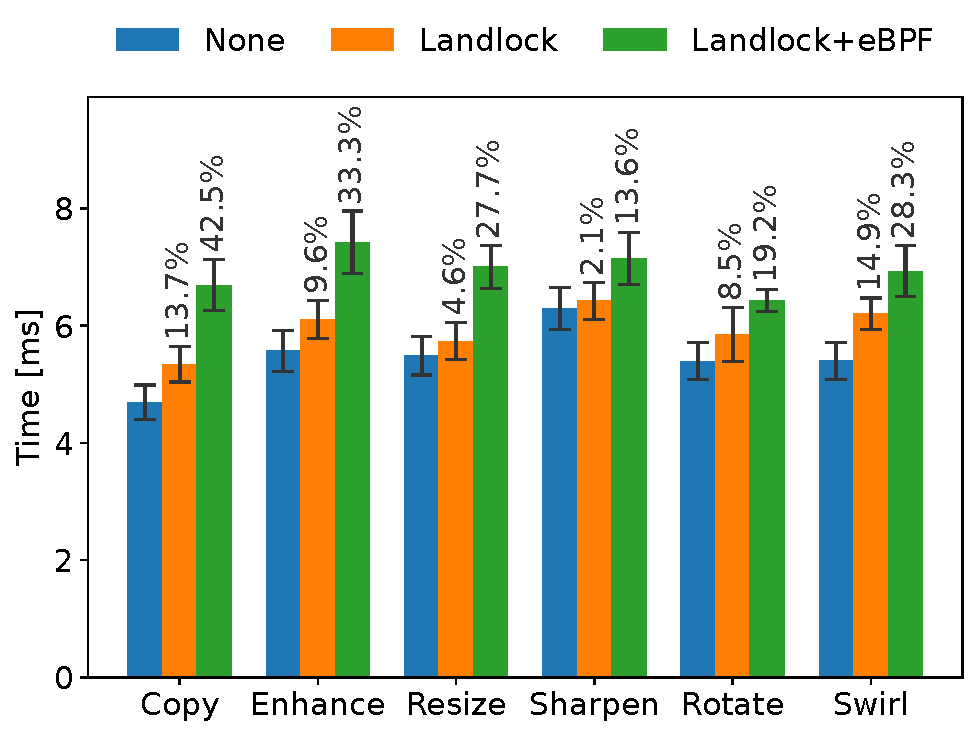
\includegraphics[width=\linewidth]{chapters/dmng/fig/convert_small.pdf}
    \caption{32x32 image resolution}
    \label{fig:convert-small-times}
  \end{subfigure}
  \begin{subfigure}[b]{0.5\linewidth}
    \centering
    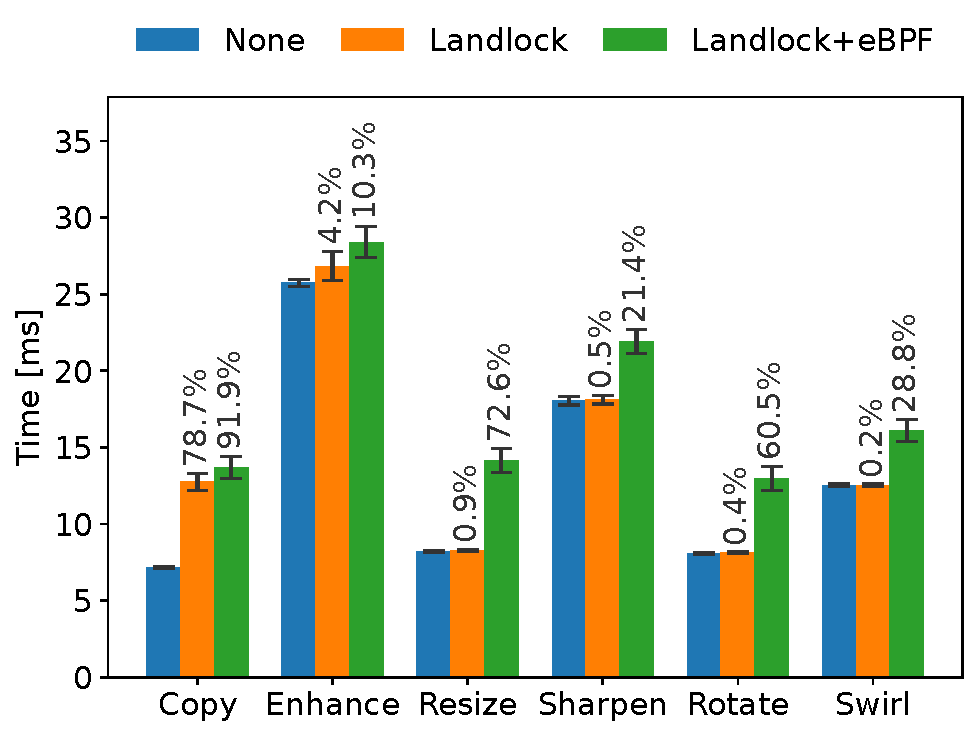
\includegraphics[width=\linewidth]{chapters/dmng/fig/convert_med.pdf}
    \caption{640x480 image resolution}
    \label{fig:convert-med-times}
  \end{subfigure}
  \begin{center}
    \begin{subfigure}[b]{0.5\linewidth}
      \centering
      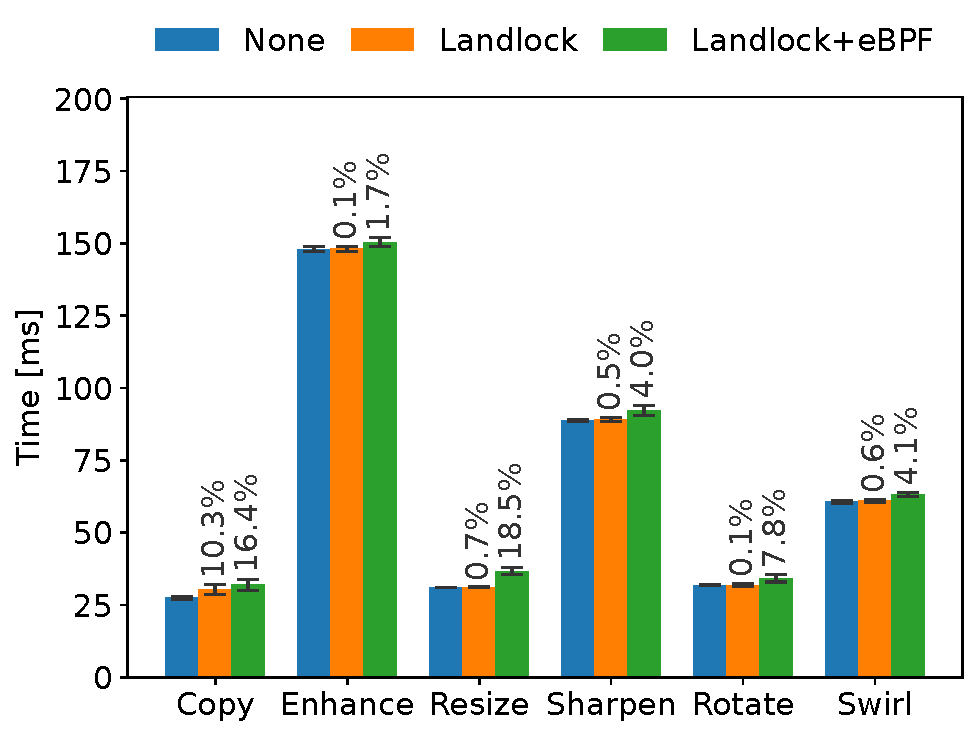
\includegraphics[width=\linewidth]{chapters/dmng/fig/convert_large.pdf}
      \caption{1920x1080 image resolution}
      \label{fig:convert-large-times}
    \end{subfigure}
  \end{center}
  \caption[Latency of image processing operations]{
      Latency associated with various operations for an image
      processing application
  }
  \label{fig:convert-times}
\end{figure*}

\begin{figure*}[t!]
  \begin{subfigure}[b]{0.5\linewidth}
    \centering
    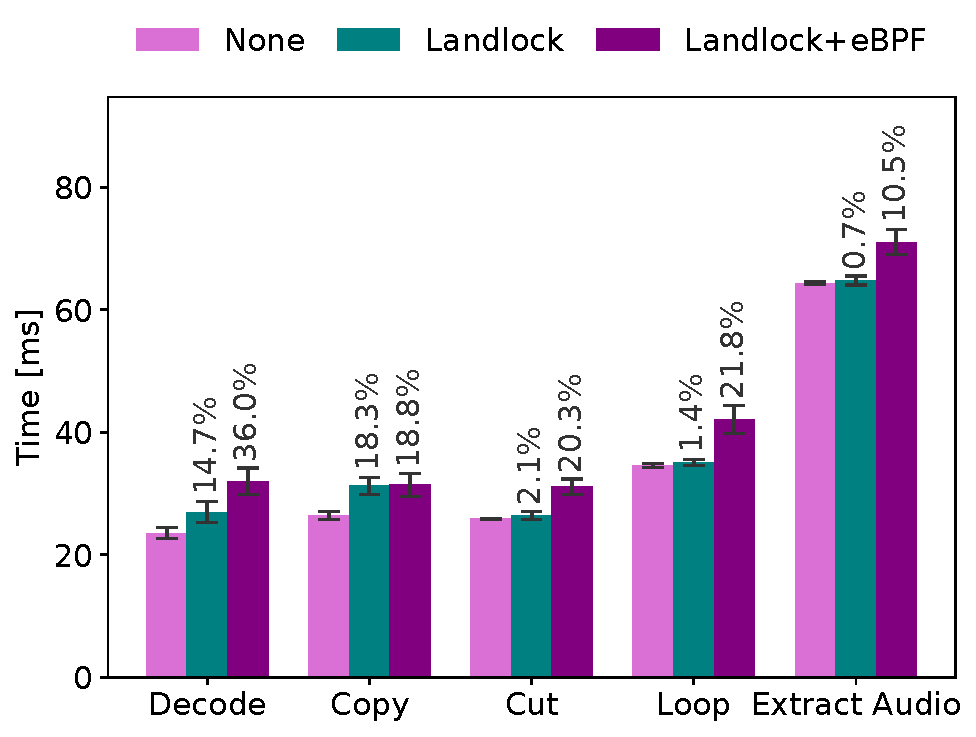
\includegraphics[width=\linewidth]{chapters/dmng/fig/ffmpeg_1.pdf}
    \caption{6 seconds 480p video}
    \label{fig:ffmpeg1-times}
  \end{subfigure}
  \begin{subfigure}[b]{0.5\linewidth}
    \centering
    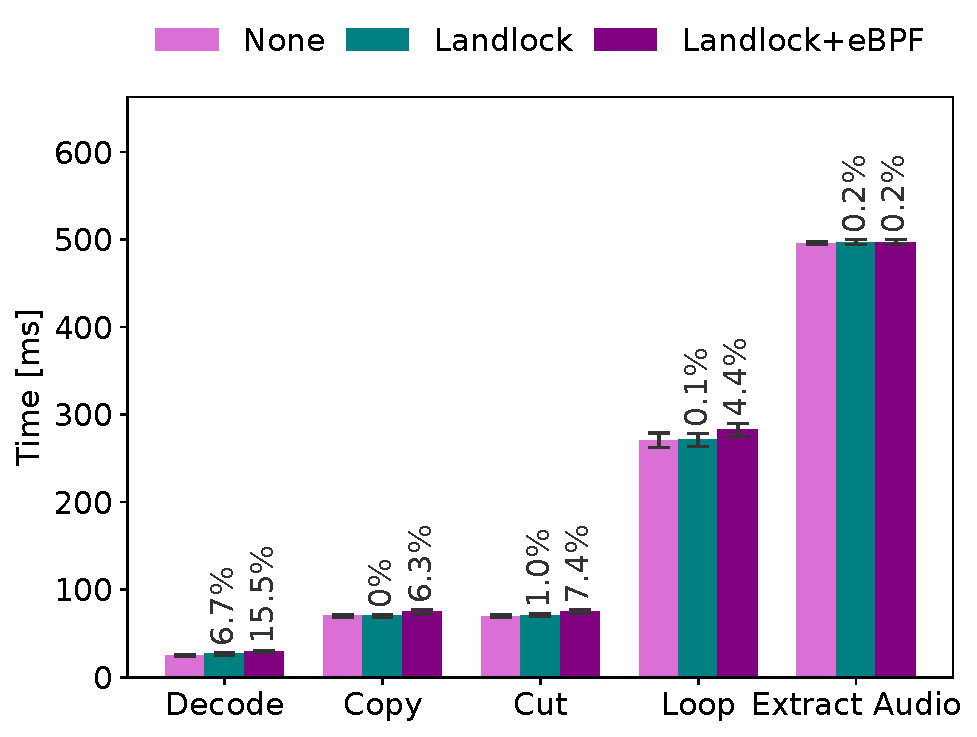
\includegraphics[width=\linewidth]{chapters/dmng/fig/ffmpeg_10.pdf}
    \caption{1 minute 480p video}
    \label{fig:ffmpeg10-times}
  \end{subfigure}
  \begin{center}
    \begin{subfigure}[b]{0.5\linewidth}
      \centering
      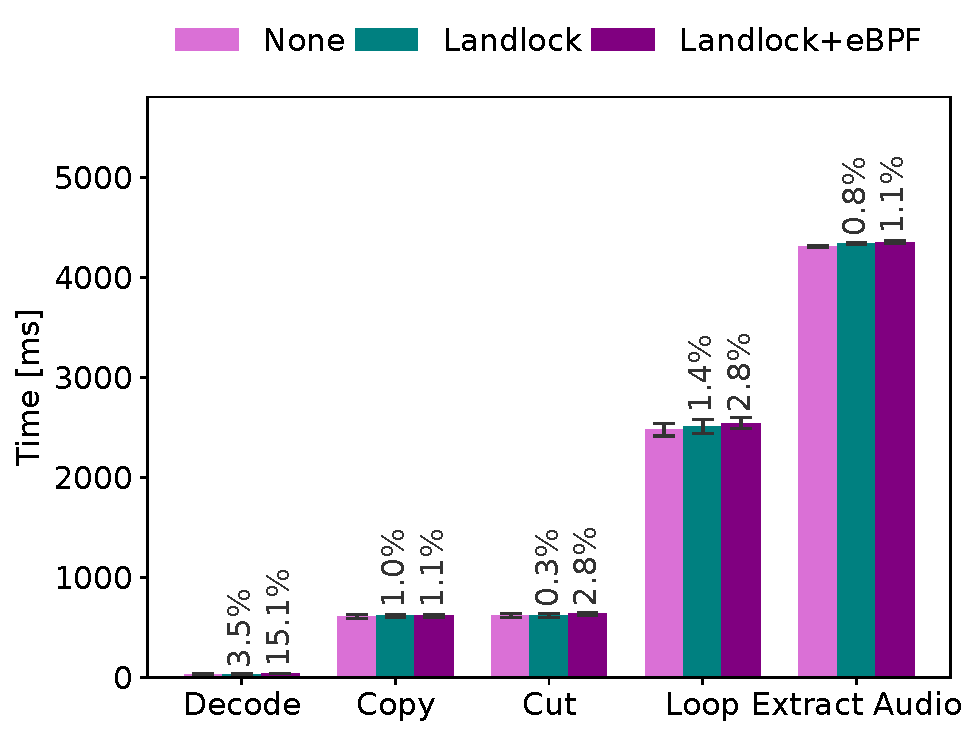
\includegraphics[width=\linewidth]{chapters/dmng/fig/ffmpeg_100.pdf}
      \caption{10 minutes 480p video}
      \label{fig:ffmpeg100-times}
    \end{subfigure}
  \end{center}
  \caption[Latency of video processing operations]{
      Latency associated with various operations for a video
      processing application
  }
  \label{fig:ffmpeg-times}
\end{figure*}

The first set of experiments focuses on image processing. In detail,
the application leverages {\em convert} to copy, enhance, resize,
sharpen, rotate and swirl images with 32x32, 640x480 and 1920x1080
resolutions. The results are shown in
Figure~\ref{fig:convert-times}. Inevitably, sandboxing introduces a
slight degradation of latency compared to a scenario without
protection.  However, the overhead is non-negligible only for
short-lived operations that last less than 10 ms, a duration that is
considerably less than the average network delay. When instead
eBPF-based monitoring is enabled, the data show worse latency
degradation, especially for operations that last less than
50~ms. Remarkable is the case 640x480, in which the average operation
overhead associated with eBPF-based monitoring is 47.6\%.

The second set of experiments focuses on video processing. In detail,
the application leverages {\em ffmpeg} to decode, copy, cut, loop and
extract audio from videos with 480p resolution and with 6 seconds, 1
minute, and 10 minutes duration respectively. The results are shown in
Figure~\ref{fig:ffmpeg-times}. The overhead introduced by sandboxing
is perceptible only for the decode and copy operations on the shortest
video (6 seconds). However, it never exceeds 18.3\%. As expected, the
overhead becomes practically negligible for operations that take
longer than 100 ms. The same considerations extend to the eBPF-based
monitoring, which again confirms to be associated with more
degradation compared to the Landlock-only solution.

%%% Local Variables:
%%% mode: latex
%%% TeX-master: "../main"
%%% End:

\section{Related work}
\label{dmng:sect:related-work}

Several research works have highlighted the importance of sandboxing
and isolation techniques in modern software~\cite{kim2013practical,
  lsm_fra, berman1995tron, RLBox, seapp, ALBANESE2020934}. Indeed,
sandboxing plays a key role in many plaftorms (e.g., Linux, Windows,
iOS, Android), and is integrated in widely used software such as
browsers (e.g., Chrome~\cite{chromium-sandbox},
Firefox~\cite{firefox-sandbox}), service managers (e.g.,
Systemd~\cite{systemd-sandbox}) and document viewers (e.g.,
Acrobat~\cite{acrobat-sandbox}).

With specific reference to the cloud scenario, many recent proposals
have investigated the use of sandboxing to mitigate
vulnerabilities~\cite{natisand, cage4deno, enhance-wasm-sandbox,
  sanddriller-staicu, staicu2021bilingual, binwrap, zimmermann-risks,
  npm-malicious-update}. In {\em NatiSand}~\cite{natisand} and {\em
  Cage4Deno}~\cite{cage4deno} the authors modify the Deno runtime to
control the permissions available to applications running native
code. {\em BinWrap}~\cite{binwrap} proposes similar measures to
restrict the permissions available to Node.js native add-ons.  {\em
  SandDriller}~\cite{sanddriller-staicu} describes an approach based
on dynamic analysis for detecting sandbox escape vulnerabilities for
Node.js applications. Zimmermann et al.~\cite{zimmermann-risks} and
Ferreira et al.~\cite{npm-malicious-update} study the risks associated
with vulnerable or malicious third-party dependencies and propose
possible install (and update) time countermeausures. In general, all
the previous proposals address the issues associated with a specific
runtime ecosystem. Conversely, we aim to secure applications
independently of their build toolchain or runtime.

Virtual machines and containers are two fundamental technologies in
modern cloud architectures. Both permit to virtualize resources and
execute applications in an isolated environment. Virtual machines
ensure stronger security guarantees at the cost of higher resource
utilization with respect to containers. The main reason is that
applications executed in separate virtual machines have a distinct set
of resources and do not share the same
kernel~\cite{casola-optimization, CASOLA2018235}.  With specific
reference to our scenario, both these technologies are associated with
coarse granularity. Indeed, when working with them developers grant
the application access to volumes rather than single resources. So, we
provide a complementary approach to enable the introduction of
fine-grained, per-resource access rules.

Modern industrial platforms like Cilium~\cite{cilium} and
Falco~\cite{falco} rely on eBPF as the primary means to enforce
security policies in cloud applications. Cilium provides networking,
observability, and security functions for container workloads, while
Falco implements a threat detection engine for clusters. Both
solutions are enterprise-oriented, hence the developer may find
difficult to set up fine-grained policies leveraging them. Moreover,
as already mentioned in the chapter, the performance of eBPF-based
solutions is associated with large variability when fine-grained rules
are used~\cite{falco-overhead}. Therefore, we propose to complement
these solutions by assisting the developer in the generation of least
privilege security policies and using recent sandboxing technologies
like Landlock, to reduce the overhead and strengthen the security
boundary of the application.

%%% Local Variables:
%%% mode: latex
%%% TeX-master: "../main"
%%% End:

\section{Conclusions}
\label{dmng:sect:conclusions}

The mitigation of security bugs and vulnerabilities that affect cloud
applications is an important topic. In this chapter, we presented an
approach to support the introduction of security policies to restrict
the file system resources available to an application. To facilitate
adoption, a central aspect in our proposal is the support to policy
generation. We provide an open source tool to generate and customize
least privilege policies leveraging the powerful, yet complex, ptrace
and eBPF kernel technologies.  Compared to virtualization technologies
such as VMs and containers, which are associated with coarse
granularity, we demonstrate that our proposal enables the introduction
of fine-grained, per-resource access rules. The experiments showcase
the capability of our approach to mitigate severe CVEs at the cost of
limited, often negligible, overhead.

While currently the protection is limited to the file system, the
isolation can be extended to other subsystems (e.g., the network).
This is a promising line of research we aim to explore in the future.

%%% Local Variables:
%%% mode: latex
%%% TeX-master: "../main"
%%% End:


\section*{Availability}
The source code and artifacts produced for the evaluation of
our proposal are available open source at
\url{https://github.com/unibg-seclab/dmng}


\chapter[Enhancing the Sandbox of WebAssembly Runtimes]{Enhancing the Sandbox of \\ WebAssembly Runtimes}
\label{chap:wasm}
\colorlet{punct}{red!60!black}
\definecolor{background}{HTML}{EEEEEE}
\definecolor{delim}{RGB}{20,105,176}
\definecolor{types}{RGB}{255,0,0}
\definecolor{myBrickRed}{RGB}{203,65,84}

% circle shapes
\DeclareRobustCommand{\blackcircle}[1]{\tikz[baseline=-0.3em]{
		\node[shape=circle,scale=0.55,fill=black,text=white,draw,inner sep=2pt] (char) {#1};}}
\DeclareRobustCommand{\whitecircle}[1]{\tikz[baseline=-0.3em]{
		\node[shape=circle,scale=0.65,fill=white,text=black,draw,inner sep=2pt] (char) {#1};}}

%%% Local Variables:
%%% mode: plain-tex
%%% TeX-master: t
%%% End:


\section{Introduction}\label{intro}

While effective in restricting filesystem access to an entire
microservice, the approach described in the previous chapter can be
further improved by considering the specifics of emerging technologies
that enable finer-grined compartmentalization of cloud applications.

WebAssembly (Wasm)~\cite{haas2017bringing} is a popular binary
instruction format that enables the execution of untrusted code in a
safe, isolated environment. Moreover, it is a portable compilation
target for different languages, and can be executed efficiently on a
wide range of platforms without the need of dedicated hardware. Wasm
was originally meant to be run inside web browsers, but given the
considerable advantages it brings, many runtimes that allow
execution in standalone mode have been developed recently. Popular
examples are Wasmtime, WasmEdge, Wasmer, and WAMR.

To answer the developers' need to access resources of the host
system from within the runtime, a standardization effort called
WebAssembly System Interface (WASI)~\cite{wasi} is undergoing.
Its goal is to provide a stable and multi-platform system interface. To be WASI-compliant, each runtime must implement
all the calls defined in the interface with dedicated functions, which
are named hostcalls. However, implementing these functions is
non-trivial, since (i) the code must not introduce violations to the
Wasm memory model, and (ii) it is possible to break the separation
between the system and the isolated environment in which the Wasm module is
executed. The solution adopted by current runtimes leverages
WASI Libc~\cite{wasi-libc}, a library providing POSIX-compatible APIs
built on top of hostcalls.

% The first proposal of a system interface was the file system one.
Currently, every WASI-compliant runtime implements the proposed file system
interface with a libpreopen-like layer~\cite{libpreopen}. Whenever the runtime
receives a request to open a file, it first checks whether the path
belongs to the authorized list of directories, then it opens the file
on behalf of the Wasm program, redirecting the content to the caller.
Previous work~\cite{johnson2022wave,
  bosamiya2022provably, lehmann2020everything} proved the approach
to be error-prone, leaving the system unprotected when a vulnerability
was introduced in a hostcall wrapper (Figure~\ref{fig:wasi}). Moreover,
this approach provides limited flexibility, as it is associated with
directory-based granularity instead of file-based. Lastly, in order to audit
the policy regulating resource access, one must find the permissions
by looking at the code.
We claim that there is no practical advantage in having several
implementations of the same access control checks for different
runtimes. Our idea is to replace the user-space runtime-specific
security checks with a single in-kernel implementation that leverages
eBPF~\cite{bpf-lsm-hooks}.
There are considerable advantages in doing so: (i)~it permits to decouple the implementation of hostcall wrappers
and the access control details, minimizing the risk of bugs~\cite{kehoe2022ebpf,seapp, cage4deno},
(ii)~it enables the introduction of per-module policies with file-based
granularity, and (iii)~it fulfills Wasm's promise of portability as eBPF programs are portable across different kernel versions~\cite{andrii2021bpfCORE} and also operating systems, thanks
to Microsoft's undergoing effort to port eBPF to
Windows~\cite{ebpf-windows}.
% In the following we describe the threat model and our efforts to
% integrate eBPF into production Wasm runtimes. Finally, we discuss
% our results.

\section{Threat model}
\label{sect:wasm:threat-model}

Our assumptions reflect the threat model employed by Wasm runtimes. We
assume that the code executed by the runtime is either untrusted or it
is trusted but potentially affected by security vulnerabilities due to
bugs. The goal of the attacker providing the code is to bypass the
security checks enforced by the runtime to get access to the host file
system. To fulfill this objective, the attacker can leverage the
interface provided by WASI and send any argument. Runtime escapes
caused by memory corruption or alteration of the program flow are out
of scope of our work, since protection can be provided by other
existing solutions (e.g., ~\cite{bosamiya2022provably}).

\begin{figure}[t!]
	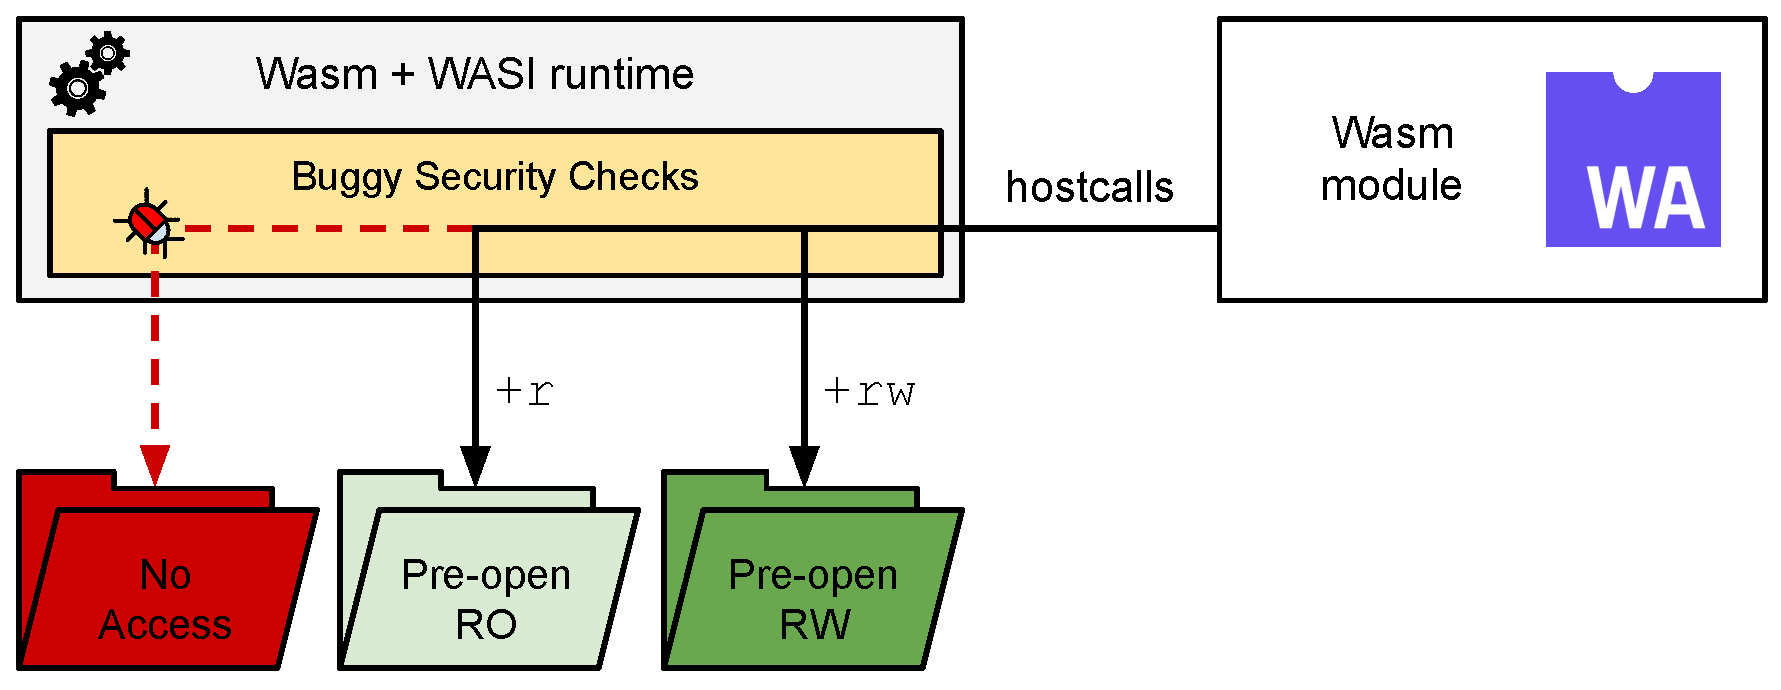
\includegraphics[width=\columnwidth]{chapters/wasm/fig/wasi}
	\caption[Current implementation of WASI by runtimes]{
    Current implementation of WASI by runtimes. A bug present in a
    hostcall wrapper permits the module to read the unauthorized
    directory on the left (red dotted arrow)
  }
	\label{fig:wasi}
\end{figure}


%%% Local Variables:
%%% mode: latex
%%% TeX-master: "../main.tex"
%%% End:

\section{Architecture}\label{design}

Our analysis starts from the scenario illustrated in
Figure~\ref{fig:wasi}. Currently, WASI-compliant runtimes
implement dedicated user-space wrappers to enforce the
security boundaries of hostcalls. File system access is granted by the
user on a set of pre-opened directories that are specified via CLI
before the Wasm module is run (e.g., with the {\tt -{}-dir} option).
We follow a similar approach, asking the user to state the permissions
of each Wasm module in a JSON policy file. Contrary to existing
runtimes, permissions can be granted with file-based granularity.
Three permissions are available: (i) {\tt read} to open and read a
file, (ii) {\tt write} to modify, truncate and append content to a
file, and (iii) {\tt delete} to remove the file. When permissions are
related to a directory, {\tt read} translates to listing its content,
{\tt write} allows to create and delete files within it. We extended the Wasmtime
and WasmEdge runtimes to load the policy at startup, and, instead of
pre-opening the directories available to the Wasm module, we enforce
the policy with eBPF. eBPF code is split into programs attached to a
kernel- or user-space function called {\em hook point} and executed
whenever the hook is reached. Programs have visibility of function
parameters, they can persist state and share it with user space using
{\em maps}, and most of all they can enforce security checks based on
this information. Once the policy is encoded inside the map and the
eBPF programs are loaded, the runtime instantiates the
Wasm module selected by the user (arrow \blackcircle{A} in
Figure~\ref{fig:arch}). At this stage, the modified runtime invokes
a dedicated user probe specifying as a parameter the policy
that confines the loaded Wasm module~(\blackcircle{B}). The argument
is captured by a dedicated eBPF program that also annotates the
identifier of the thread running the Wasm interpreter in a tracing
map. We highlight that the policy is activated before the runtime
executes the module (i.e., before untrusted code is interpreted).
The consequence is that, from this point on, all the hostcalls
performed by the Wasm module are restricted by our eBPF programs
(arrows~\whitecircle{1}, ~\whitecircle{2}). The eBPF programs that make the
security decisions are evaluated every time a file-related kernel
security hook is reached (e.g., {\tt security\_file\_open}), and any
access decision is enforced at kernel level. When an unauthorized
request is performed by the Wasm code~(\whitecircle{3}), the related
eBPF program detects the violation and denies the request, returning
to the caller a permission denied error. When the execution of untrusted 
Wasm code terminates, another eBPF program is responsible for 
removing the access restriction from the thread executing the Wasm
runtime. No further intervention from the runtime is required, as the
maps and the eBPF programs are automatically removed from the kernel
immediately after the process running the runtime terminates.

This architecture offers several advantages. First, it eliminates the
risks coming from buggy user-space security checks (e.g., wrong
filepath resolution~\cite{parentfix}, wrong directory
removal~\cite{removedirfix}). Then, by leveraging kernel hook
points~\cite{bpf-lsm-hooks}, our approach allows the runtime developer
to focus on the interaction between Wasm code and the memory unsafe
system call, leaving aside authorizations and policy-related issues.
Lastly, access constraints can be audited by simply looking at the
JSON policy, instead of inspecting the code.

\begin{figure}[t!]
     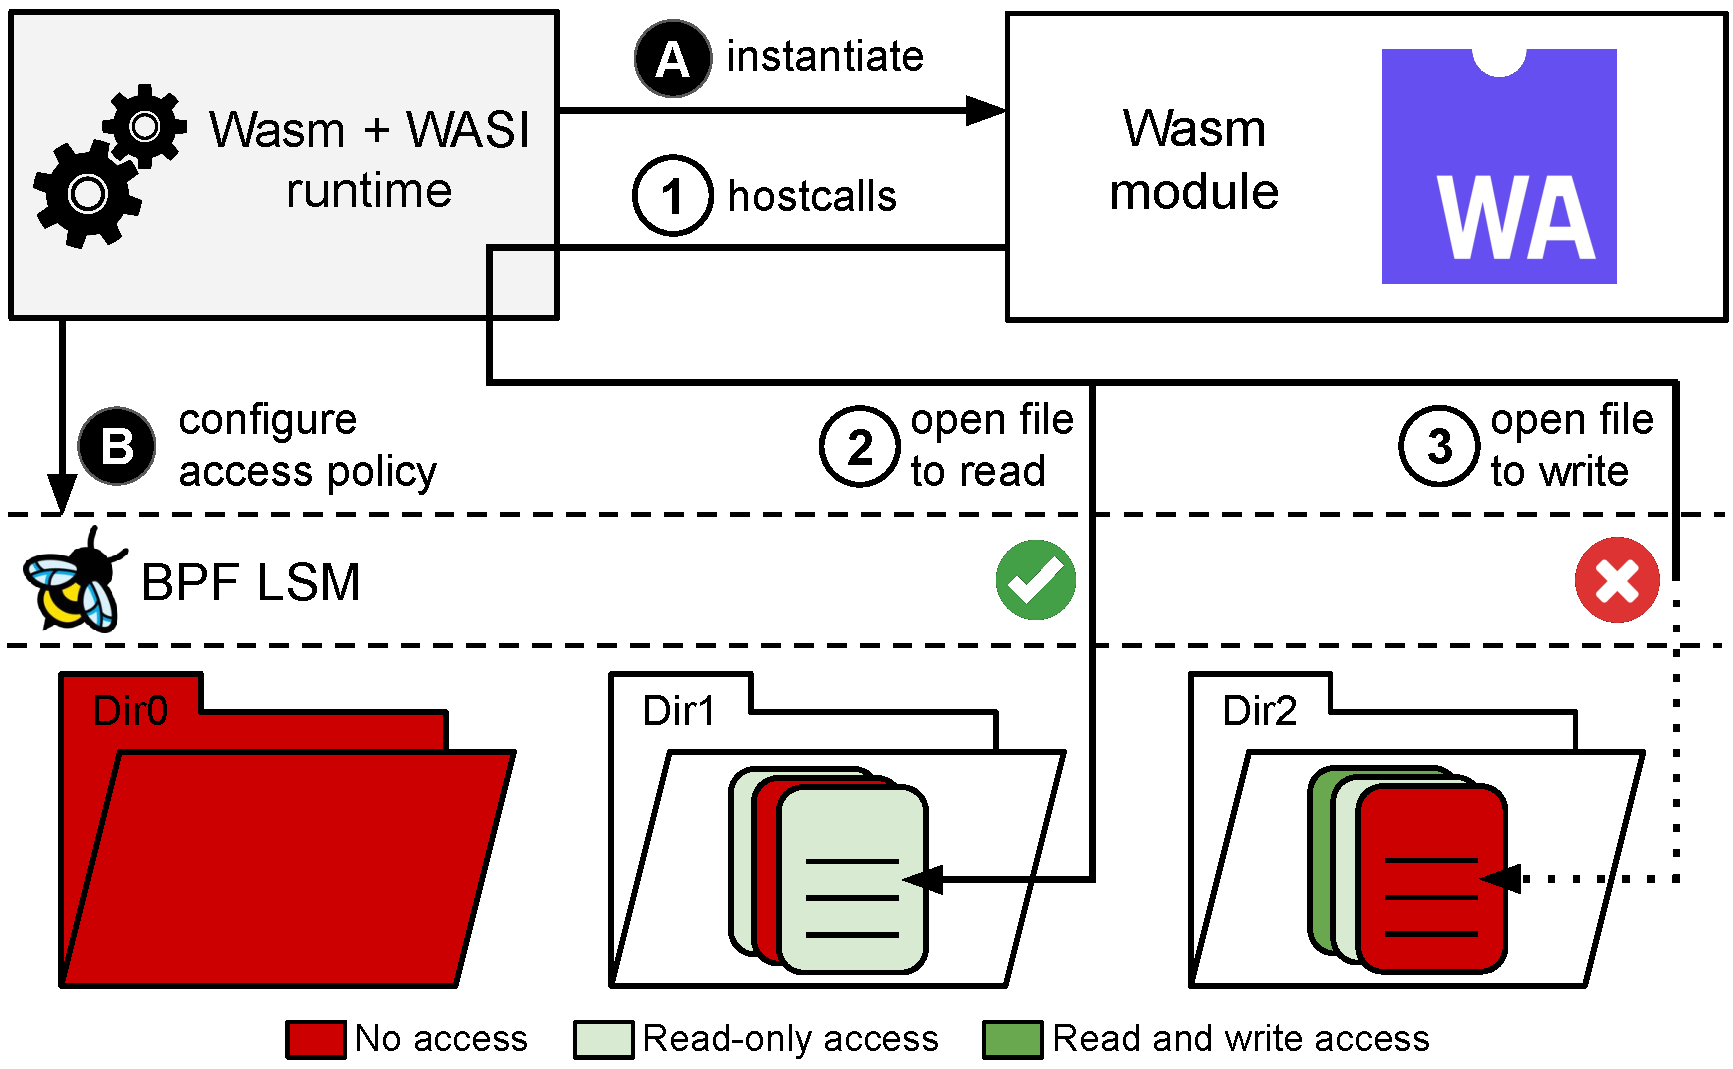
\includegraphics[width=\columnwidth]{chapters/wasm/fig/wasi-bpf}
     \caption[eBPF-based restriction of Wasm modules]{
          eBPF-based restriction of Wasm modules. The runtime
          instantiates the Wasm module (\blackcircle{A}), and
          configures the associated policy calling the traced user
          probe (\blackcircle{B}). After the Wasm module is run, all
          the hostcalls issued by the program (\whitecircle{1}) are
          restricted by eBPF (\whitecircle{2}, \whitecircle{3})
     }
     \label{fig:arch}
\end{figure}


%%% Local Variables:
%%% mode: latex
%%% TeX-master: "../main.tex"
%%% End:

\section{Experiments \label{sec:exp}}

To investigate the overhead introduced by our solution we implemented
it in WasmEdge and Wasmtime, two industrial state-of-the-art Wasm
runtimes. The evaluation has been performed in the following test
environment: an Ubuntu 22.04 LTS server powered by an AMD Ryzen 2950X
CPU with 16 cores, 128 GB RAM, and 2 TB SSD. %No kernel
%upgrade or modification was required, as eBPF is already available in
%the default OS image.
In order to assess the performance, we tested one of the most popular
binaries that can be compiled to Wasm with support to WASI: {\tt uutils
coreutils}, the porting of the coreutils in Rust~\cite{coreutils-repo}.
First, we compiled the coreutils with the {\tt wasm32-wasi}
target, and applied runtime-specific optimization
(with {\tt wasmedgec}~\cite{wasmedgec} for WasmEdge and with
{\tt wasmtime compile}~\cite{wasmtimecompile} for Wasmtime) to further
speed up the code. Then, we reproduced
the benchmarks reported in the coreutils repository, with the
exception of those that are not portable to WASI due to temporary lack
of support (e.g., the {\tt dd} utility needs to spawn threads, a
feature that is yet to be implemented~\cite{wasi-threads}). Finally, we
repeated the experiments with our protection in place. The Hyperfine
benchmarking tool~\cite{hyperfine} was used to log measures, and 1000
runs were performed (with 100 warmups). As shown from the results in Table~\ref{table:exp}, our approach introduces
a limited overhead, ranging from an additional 0.12\% to 6.30\% for
WasmEdge, and from 0.28\% to 14.29\% for Wasmtime. As expected, the
highest overhead is experienced by short-living utilities (e.g.,
{\tt head}). We also observe that there are notable differences
between the WasmEdge and Wasmtime test execution time for some utilities (e.g.,
{\tt ls} and {\tt cut}); from our analysis these differences are
mostly caused by the specific post-compilation optimizations.

\begin{table}[!t]
	\setlength{\tabcolsep}{0.38cm}
	\begin{tabular*}{\columnwidth}{l r r r r}
		\toprule
		{\bf Utility} & {\bf WasmEdge} & {\bf WasmEdge*} & {\bf Wasmtime} & {\bf Wasmtime*}\\
		\midrule
		{\tt head}  &   32 &   34 (+6.25\%) &   14 &   16 (+14.29\%) \\
		{\tt sum}   &  134 &  137 (+2.24\%) &  130 &  136  (+4.62\%) \\
		{\tt tac}   &  149 &  150 (+0.67\%) &  152 &  155  (+1.97\%) \\
		{\tt wc}    &  285 &  287 (+0.70\%) &  309 &  310  (+0.32\%) \\
		{\tt shuf}  &  298 &  300 (+0.67\%) &  356 &  358  (+0.56\%) \\
		{\tt ls}    &  512 &  526 (+2.73\%) & 1077 & 1113  (+3.34\%) \\
		{\tt seq}   & 1155 & 1157 (+0.17\%) & 1526 & 1533  (+0.46\%) \\
		{\tt cut}   & 1403 & 1411 (+0.57\%) &  359 &  360  (+0.28\%) \\
		{\tt join}  & 1601 & 1603 (+0.12\%) & 2054 & 2065  (+0.54\%) \\
		{\tt split} & 4416 & 4694 (+6.30\%) & 4933 & 4998  (+1.32\%) \\
		\bottomrule
	\end{tabular*}
	\caption[Average execution time of coreutils with and without our approach]{
		\label{table:exp} Average execution time in {\em ms} of the
		coreutils without and with* our approach (\% overhead in
		parenthesis)
	}
\end{table}
%%% Local Variables:
%%% mode: latex
%%% TeX-master: "../main.tex"
%%% End:

\section{Related work}
\label{wasm:rel_works}

There are several successful solutions that leverage Wasm to sandbox
untrusted code~\cite{RLBox, ewasm, sledge}. RLBox~\cite{RLBox} is a
framework that facilitates the isolation of third-party libraries in
pre-existing software. eWASM~\cite{ewasm} optimizes the execution of
Wasm in embedded systems with constrained resources. Sledge~\cite{sledge}
enables efficient Wasm-based serverless execution on the
edge. The use of our approach for restricting access to the file
system within these frameworks can strengthen their security
assurance.

The memory safety guarantees of Wasm depend on the runtime
implementation~\cite{lehmann2020everything}. Hence, Bosamiya et
al.~\cite{bosamiya2022provably} explore the problem of producing
provably safe sandboxes. WaVe~\cite{johnson2022wave} explains that any
interaction with the unsafe interfaces exposed by WASI can
introduce security and safety violations. Thus, the authors proposed
a verified secure runtime system
implementing WASI. However, both works require to redesign the runtime
toolchain, while our solution can be directly integrated into existing
runtimes.
%However, both proposals rely on implementing a new runtime, 
%while our approach integrates with existing runtimes used in the industry.

The academic and industrial communities have investigated the use of eBPF
for the isolation of software~\cite{findlay2020bpfbox, findlay2021bpfcontain,
cilium-repo, falco}.
{\em BPFBox}~\cite{findlay2020bpfbox} and {\em BPFContain}
~\cite{findlay2021bpfcontain} use an eBPF daemon to confine processes and
services.
{\em Cilium}~\cite{cilium-repo} provides eBPF-based networking, observability
and security for container workloads.
{\em Falco}~\cite{falco} enables lightweight threat detection in the
cluster. These solutions highlight the potential of eBPF, and provide
a simple and flexible confinement of system resources. However, they
focus on containers or services, while our solution aims at enforcing
fine-grained per-sandbox policies.

% say something about the match between WASM & eBPF portability ???

%%% Local Variables:
%%% mode: latex
%%% TeX-master: "../main.tex"
%%% End:

\section{Conclusions}

The results achieved by our approach are promising: not only it
permits to introduce fine-grained policies to restrict file system
access, it is also associated with a limited overhead which is aligned
with the needs of a modern sandbox. The protection is currently
applied only to the file system, but our approach has the potential to
be extended also to network sockets, which are in the first stage of
the standardization process~\cite{wasi-sockets}. We believe this
could be an interesting line of research for future work.

%%% Local Variables:
%%% mode: latex
%%% TeX-master: "../main.tex"
%%% End:


% \begin{acks}
% We thank the reviewers for their valuable comments and feedback.
% This work was supported by the European Commission in the HE program
% within the GLACIATION project (No 101070141).
% \end{acks}


\chapter[Native Code Sandboxing for JavaScript Runtimes]{Native Code Sandboxing for \\ JavaScript Runtimes}
\label{chap:natisand}
\colorlet{punct}{red!60!black}
\definecolor{background}{HTML}{EEEEEE}
\definecolor{delim}{RGB}{20,105,176}
\definecolor{types}{RGB}{255,0,0}
\definecolor{myBrickRed}{RGB}{203,65,84}
\lstdefinelanguage{json}{
	xleftmargin=0.8em,
	basicstyle=\small\ttfamily,
	numbers=left,
	numberstyle=\scriptsize,
	stepnumber=1,
	numbersep=8pt,
	showstringspaces=false,
	breaklines=true,
	frame=lines,
	backgroundcolor=\color{background},
	literate=
	*{:}{{{\color{punct}{:}}}}{1}
	{,}{{{\color{punct}{,}}}}{1}
	{\{}{{{\color{delim}{\{}}}}{1}
	{\}}{{{\color{delim}{\}}}}}{1}
	{[}{{{\color{delim}{[}}}}{1}
	{]}{{{\color{delim}{]}}}}{1},
}

\lstdefinelanguage{javascript}{
	xleftmargin=0.8em,
	basicstyle=\small\ttfamily,
    keywords=[1]{Array},
	keywordstyle=[1]\color{blue},
	keywords=[2]{number, string},
	keywordstyle=[2]\color{red},
	extendedchars=true,
	numbers=left,
	numberstyle=\scriptsize,
	stepnumber=1,
	numbersep=8pt,
	showstringspaces=false,
	showspaces=false,
	breaklines=true,
	frame=lines,
	backgroundcolor=\color{background},
	literate=
	*{:}{{{\color{punct}{:}}}}{1}
	{,}{{{\color{punct}{,}}}}{1}
	{\{}{{{\color{delim}{\{}}}}{1}
	{\}}{{{\color{delim}{\}}}}}{1}
	{[}{{{\color{delim}{[}}}}{1}
	{]}{{{\color{delim}{]}}}}{1}
	{<}{{{\color{delim}{<}}}}{1}
	{>}{{{\color{delim}{>}}}}{1},
}


\lstdefinelanguage{rust}{
	xleftmargin=0.8em,
	basicstyle=\small\ttfamily,
	keywords=[1]{struct, Option, Vec},
	keywordstyle=[1]\color{blue},
	keywords=[2]{Policy, PolicyIdentifiers, PolicyVector, PolicyVectors, String, u32},
	keywordstyle=[2]\color{red},
	extendedchars=true,
	numbers=left,
	numberstyle=\scriptsize,
	stepnumber=1,
	numbersep=8pt,
	showstringspaces=false,
	showspaces=false,
	breaklines=true,
	frame=lines,
	backgroundcolor=\color{background},
	literate=
	*{:}{{{\color{punct}{:}}}}{1}
	{,}{{{\color{punct}{,}}}}{1}
	{\{}{{{\color{delim}{\{}}}}{1}
	{\}}{{{\color{delim}{\}}}}}{1}
	{[}{{{\color{delim}{[}}}}{1}
	{]}{{{\color{delim}{]}}}}{1}
	{<}{{{\color{delim}{<}}}}{1}
	{>}{{{\color{delim}{>}}}}{1},
}

\lstdefinelanguage{sh}{
	xleftmargin=0.8em,
	basicstyle=\small\ttfamily,
	keywords=[1]{dmng},
	keywordstyle=[1]\color{blue},
	morecomment=[f][\color{myBrickRed}][0]{\#},
	extendedchars=true,
	numbers=left,
	numberstyle=\scriptsize,
	stepnumber=1,
	numbersep=8pt,
	showstringspaces=false,
	showspaces=false,
	breaklines=true,
	frame=lines,
	backgroundcolor=\color{background},
	literate=
	*{:}{{{\color{punct}{:}}}}{1}
	{,}{{{\color{punct}{,}}}}{1}
	{\{}{{{\color{delim}{\{}}}}{1}
	{\}}{{{\color{delim}{\}}}}}{1}
	{[}{{{\color{delim}{[}}}}{1}
	{]}{{{\color{delim}{]}}}}{1}
	{<}{{{\color{delim}{<}}}}{1}
	{>}{{{\color{delim}{>}}}}{1},
}

\newcommand{\twoRows}[2]{\begin{tabular}{@{}c@{}}#1 \\ #2\end{tabular}}

% Two row cell in table
\newcommand{\pap}{NatiSand\xspace}

\newcommand{\generation}{\color{blue}\input{src/proposal/generation}\color{black}}

% do not count empty lines in listings
\makeatletter
%
\lst@Key{countblanklines}{true}[t]%
    {\lstKV@SetIf{#1}\lst@ifcountblanklines}
%
\lst@AddToHook{OnEmptyLine}{%
    \lst@ifnumberblanklines\else%
       \lst@ifcountblanklines\else%
         \advance\c@lstnumber-\@ne\relax%
       \fi%
       \fi}
%    
\lst@AddToHook{OnEmptyLine}{\addtocounter{lstnumber}{-1}}% Remove line number increment from listings
%    
\makeatother



% DESIGN OBJECTIVES
\newcommand{\objintegration}{\textbf{O1}\xspace}
\newcommand{\objeasy}{\textbf{O2}\xspace}
\newcommand{\objfinegrained}{\textbf{O3}\xspace}
\newcommand{\objpolicy}{\textbf{O4}\xspace}
\newcommand{\objmitigation}{\textbf{O5}\xspace}
\newcommand{\objoverhead}{\textbf{O6}\xspace}

% circle shapes
\DeclareRobustCommand{\whitecircle}[1]{\tikz[baseline=-0.3em]{
		\node[shape=circle,scale=0.6,minimum size=0.6cm,draw,inner sep=1pt] (char) {\LARGE #1};}}
\DeclareRobustCommand{\graycircle}[1]{\tikz[baseline=-0.3em]{
		\node[shape=circle,scale=0.6,minimum size=0.6cm,fill=gray!70,text=white,draw=gray!70,inner sep=1pt] (char) {\LARGE #1};}}
\DeclareRobustCommand{\blackcircle}[1]{\tikz[baseline=-0.3em]{
		\node[shape=circle,scale=0.6,minimum size=0.6cm,fill=black,text=white,draw,inner sep=1pt] (char) {\LARGE #1};}}

% marks
\newcommand{\cmark}{\text{\ding{51}}}
\newcommand{\xmark}{\text{\ding{55}}}

       
\section{Introduction}
\label{sect:introduction}

JavaScript (JS) and TypeScript (TS) are popular choices for the
implementation of web applications. This success is motivated by their
flexibility, since both are simple to use for the development of
frontend and backend services, and by the vast ecosystem of open
source packages that are available. For instance, the sole {\em npm
  registry} collects more than 1.3 million
packages~\cite{npm-registry}.

The execution of JS code on the server-side is enabled by a {\em JS
  runtime}.  Since its introduction in 2009, Node.js~\cite{node} has
been the de facto solution selected by developers, but recently
Deno~\cite{deno} and Bun~\cite{bun} have received considerable
attention by the community. While the three platforms provide
distinctive features, they all depend on a key external component,
namely the {\em JS engine}, V8~\cite{v8-site} in the
case of Node.js and Deno, JavaScriptCore~\cite{javascriptcore} in the
case of Bun. The engine is a sophisticated software that securely
renders the JS code in an isolated sandbox. Runtimes extend the engine
providing components to access resources and functions that are not
directly available to the web application from within the
sandbox~\cite{node-api, deno-api}. Prominent examples are the
functions to access the network and to read/write the
filesystem. Runtimes also provide support for the execution of native
code -- i.e., running binary programs installed on the host operating
system and calling functions from the available shared libraries.

The support provided by the runtime for the execution of native code
greatly simplifies the work of the developer building the backend of a
web application. However, the APIs enabling access to system resources
and the execution of native code also raise security concerns, since
they effectively break the isolation between the JS application and
the host OS. The ability to control the resources accessible to a JS
program was indeed one of the reasons that led to the creation of Deno
in 2018~\cite{nodejs-regret}, and the solution identified by the
community was to configure the resources available to an application
with simple permission flags~\cite{deno-permissions}. This change also
influenced the design of Node.js, which introduced a similar
flag-based control model\footnote{Node.js support for creating
  security policies is still experimental as of 2023.} two years
later~\cite{node-permissions}. Unfortunately, while permissions are
effective in restricting access to the JS application, they do not
provide isolation guarantees when native code is
executed,
leaving the host exposed to security breaches~\cite{deno-permissions}.

Previous research~\cite{staicu2021bilingual,npm-malicious-update} has
already shown that frequently JS modules depend on components written
in native languages such as C or C++.  The reuse of existing utilities
permits to take advantage of popular high performance libraries and,
in addition to performance, it minimizes the cost of
development. Notable examples are: the node-sqlite3~\cite{
  node-sqlite3} and deno-sqlite3~\cite{deno-sqlite3} database drivers;
modules to perform image/video conversions, such as
sharp~\cite{sharp}, fluent-ffmpeg~\cite{fluentffmpeg-npm} and
gm~\cite{gm-npm}; OCR engines like Tesseract~\cite{tesseract}; and the
cryptography modules relying on bcrypt~\cite{bcrypt}. The 2022 State
of Open Source Security~\cite{snyk-report} claims that each open
source JS project relies on an average of 174 third-party
dependencies; also, each project is estimated to be affected by 40
vulnerabilities when its dependencies are taken into account. Taking
into consideration that web applications in most cases process
untrusted input, the risk of security incidents is high. For instance,
we identified a sample of 32 high severity CVEs\footnote{The list is
  reported in Table~\ref{table-cve}.} that affect native code used by
popular packages (with 2.6M \mbox{downloads/week}), and allow an
adversary to corrupt the filesystem, perform privilege escalation,
execute arbitrary code, open network connections to exfiltrate data,
etc.

\paragraph*{Our contribution}

We see a security gap in the way modern JS runtimes execute native
code, as neither Node.js, nor Deno, nor Bun sandbox it.  In this chapter
we propose \natisand, a framework to provide strong isolation guarantees
against the execution of native code. In detail, \natisand allows the
developer to control on a native-component basis, access to filesystem, Inter-Process
Communication, and network, effectively reducing the risks coming from
the execution of binary programs and shared libraries. Our solution is
characterized by a compact, generic architecture that fits nicely with
modern runtimes. Internally, it leverages {\em
  Seccomp}~\cite{seccompbpf} and Linux Security Modules (LSMs), such
as {\em Landlock}~\cite{landlock} and {\em eBPF}~\cite{corbet2014eBPF}
to restrict access to protected resources. In the design of our
solution we paid attention to usability by developers; it is not
necessary to have a full understanding of its advanced security
features to use it.  The developer is only required to provide a
concise and readable JSON-formatted policy file, detailing the {\em
  ambient rights} -- i.e., the access privileges available to the
components of the web application that rely on native code. To this
end, we provide the developer a comprehensive and interactive CLI tool
to support policy generation, which, as best practice
suggests, can also be integrated into CI/CD pipelines and run against
a set of test cases~\cite{sandtrap,slimtoolkit}. Another key advantage
of our approach is that it permits to sandbox native code preserving
backward compatibility, namely it does not require to change existing
modules (including third-party dependencies) to leverage the new
security features.

We implemented \natisand and integrated it into Deno. We demonstrate the
security benefits showing how our solution mitigates a number of
recent, high-severity vulnerabilities. We performed an extensive
experimental evaluation to assess its performance. We compare the
overhead introduced by our solution to scenarios in which no native
code sandboxing is performed, and when sandboxing is achieved through
other general purpose, state of the art solutions. The experiments
show that, compared to the alternatives, \natisand exhibits substantial
performance improvements. In addition it also provides an easier
interface that does not require any specific security expertise to be
correctly configured.


%%% Local Variables:
%%% mode: latex
%%% TeX-master: "../main.tex"
%%% End:

\section{Background}
\label{sectbackground} 

This section overviews the structure of a modern JS runtime. It also
provides a concise description of the components that are used by \natisand
to build the sandbox.

\vspace{-0.52em}
\subsection{JS runtimes}
\label{sect:background-js-runtime}

JS code rendering is a complex process, involving tasks such as code
compilation, code optimization, memory allocation, runtime garbage
collection of objects no longer needed, and many others. To perform
these critical tasks, modern JS runtimes rely on {\em engines},
dedicated components implementing the ECMAScript specification that
were originally developed for web browsers. As already mentioned in
Section~\ref{sect:introduction}, Node.js and Deno embed Google's
V8~\cite{v8-site}, while Bun relies on
JavaScriptCore~\cite{javascriptcore}. The interoperability between
runtime and engine is achieved with specialized bindings, which are
defined in the {\em node:v8}~\cite{node-v8-bindings} module in the
case of Node.js, in the {\em rusty\textunderscore v8}~\cite{rusty-v8}
library for Deno, and by {\em webcore}~\cite{webcore-bindings} in Bun.

While an engine provides all the tools to securely execute JS code in
an isolated context (we call it the {\em JS context}), a development
platform requires complementary features to be fully functional. For
instance, a backend web application may need to open network
connections, handle several concurrent HTTP requests, or access the
filesystem to read configuration files. To address these requirements,
the architecture of a modern runtime extends the engine with various
runtime-specific components dedicated to the interaction with the host
system. A few well-known functions implemented following this design
pattern are: interaction with the filesystem (e.g., fs, Deno.FsFile),
creation of UNIX sockets (e.g., net), and exposure of HTTP servers
(e.g., http, Deno.serveHttp).

From the web application perspective there is no difference between
the functions defined by the ECMAScript standard, and the ones
provided by the runtime (and its
extensions)~\cite{brown2017finding,dinh2021favocado}.  However,
non-standard APIs are not served directly by the engine, but are
redirected to the runtime leveraging the aforementioned
bindings. Since these APIs deliberately permit to break the isolation
between the environment controlled by the engine and the underlying
system, JS runtimes allow developers to restrict them through the
definition of permissions~\cite{node-permissions,
  deno-permissions}. Based on the runtime, permissions work with
different granularities (e.g., single API vs set of APIs) and
different default behavior. For example, Deno uses a default-deny
model requiring the developer's explicit consent to access
system resources, with effect on multiple
APIs~\cite{deno-permissions}.

Permissions are intuitive and effective, but they do not offer
significant security guarantees when a module needs to run binary
programs, or import shared libraries to leverage cross-language
function calls~\cite{deno-permissions}. To do so, the web application
must be granted the permissions to call APIs like {\em command} or
{\em dlopen} (e.g., with {\tt allow-run} and {\tt allow-ffi}
flags in Deno). In the case of {\em dlopen}, native code is directly
copied into one of the processes owned by the runtime itself before
being executed, while with {\em command}, the runtime first delegates
to the OS the creation of a process with the {\tt clone} system call,
then performs an {\tt exec} to replace the process image and run the
desired program.  Independently of the runtime used, both APIs require
to execute code outside of the isolated context managed by the engine,
as shown in Figure~\ref{fig:js_runtime}, which means that this code
runs with the same privileges of the user executing the entire JS
application.

\begin{figure}[t]
  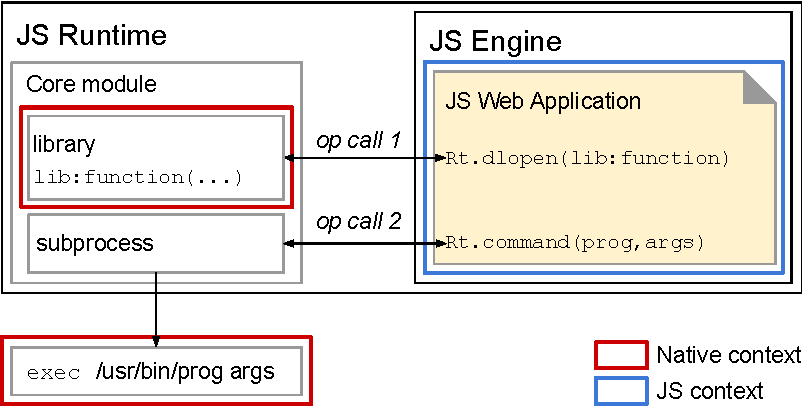
\includegraphics[width=\columnwidth]{chapters/natisand/fig/js_runtime}
  \caption[Execution of binary programs and shared libraries by JS
    runtimes]{
    Execution of binary programs and shared library functions by the
    JS runtime
  }
  \label{fig:js_runtime}
\end{figure}


\subsection{Components for resource protection}
\label{sect:background-sandboxing}

\subsubsection*{Landlock}

Landlock~\cite{landlock} is a Linux Security Module (LSM) introduced
in the kernel starting from release 5.13. The goal of Landlock is to
enable unprivileged applications to restrict their ambient rights in
accordance with the least privilege principle. Ambient rights are
specified by {\em rulesets} -- i.e., simple structures that
associate a set of permissible actions with a filesystem path (e.g.,
{\tt read} and {\tt exec} over the resources stored in {\tt
  /tmp}). Several rulesets can be combined to determine the final set
of actions available to an application. To make them effective, a call
to the {\tt landlock\textunderscore restrict\textunderscore self()}
function is performed.

The ambient rights granted by Landlock are thread-based, and are
automatically inherited by all the children subsequently created via
{\tt clone}. After a Landlock sandbox is enforced (either by self
restriction or inheritance), it is only possible to further narrow it.
It is also important to mention that Landlock is stackable, hence it
is fully composable with other LSMs already available on the host, such
as SELinux, AppArmor and SMACK.
%
Although Landlock offers a simple, yet powerful, sandboxing API,
currently, the protection offered is only limited to the filesystem.


\subsubsection*{BPF}

Berkeley Packet Filter (BPF) was originally devised in
1992~\cite{bpf-usenix93}. The goal was to provide an in-kernel
facility to filter and multiplex network packets, similarly to what
was proposed by Mogul et al.~\cite{mogul1987packer}. This version of
BPF, which is now commonly referred to as {\em classic BPF} (cBPF),
was greatly revised in 2014 resulting in {\em extended BPF}
(eBPF)~\cite{corbet2014eBPF}. The new framework provides an
environment to execute programs inside the kernel~\cite{greggebpf,
  kehoe2022ebpf}. This permits to extend the kernel safely, without
changing its source code nor loading new modules.  eBPF has a wide
variety of use cases, ranging from low overhead observability and
tracing, to load-balancing, and container runtime security
enforcement.

eBPF code is organized into compact units called
programs. Each program is attached to a specific function named {\em
  hook point}, and is executed in a non-preemptable fashion every time
the hook is reached. There are several types of hook point both in
kernel space and in user space. Valid examples
are~\cite{bpf-lsm-hooks}: system calls, kernel tracepoints, network
events, function entry/exit points, and LSM
hooks. Specifically, LSM hooks correspond to the functions
  used by LSMs (e.g. SELinux) to perform security decisions and are
  characterized by operating entirely on arguments in kernel memory.
To persist information between distinct invocations of the same
program, data structures named {\em maps} are used. Maps also permit
to share data among eBPF programs and user space
applications.

eBPF programs are written in bytecode and are loaded into the kernel
using the {\tt bpf} syscall~\cite{linux-bpf}. This is a privileged
operation that requires a few capabilities, which vary with the nature
of the program~\cite{starovoitov2020capbpf}. Briefly, {\tt CAP\_BPF}
is always required, {\tt CAP\_PERFMON} is necessary to load
tracing-related programs, while {\tt CAP\_NET\_ADMIN} is used to load
networking-related ones. After being loaded, each program undergoes a
two-phase process comprising {\em program verification} and {\em JIT
  compilation}. The former is required to guarantee that the program
is safe to execute by the kernel. The second phase instead ensures the
bytecode is optimized, hence it can be run as efficiently as compiled
kernel code on the underlying architecture. In case no errors are
raised, the eBPF program is attached to the proper hook and it is ready
to be executed.

Modern eBPF development is facilitated by the presence of {\em
  frontends}. These frameworks permit to write eBPF programs in a C
dialect, and also assist the developer in automatically performing the
steps needed to load and attach the programs to the intended hooks
(see Figure~\ref{fig:bpf_sandbox}). In our work we rely on {\em
  libbpf}~\cite{libbpf-doc}, a modern library leveraging the {\em
  Compile Once-Run Everywhere} (CO-RE)
approach~\cite{andrii2020bpfCORE}, which ensures that the bytecode
produced at compile time works correctly across different kernel
versions.

\begin{figure}[t]
  \centering
  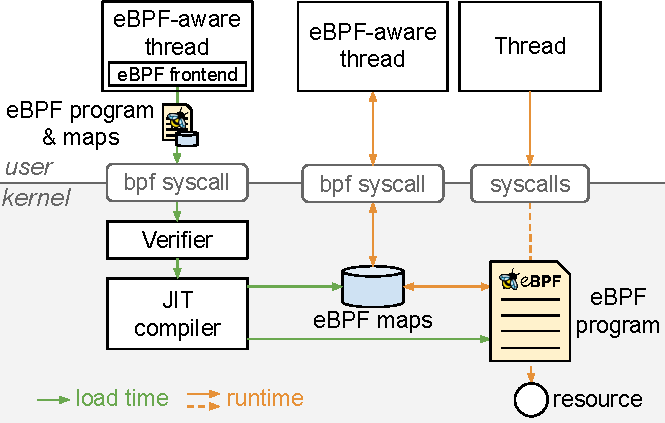
\includegraphics[width=0.9\columnwidth]{chapters/natisand/fig/bpf_bg}
  \caption{Overview of the eBPF architecture}
  \label{fig:bpf_sandbox}
\end{figure}

\subsubsection*{Seccomp}

Seccomp~\cite{seccompbpf} is a mechanism
provided by the Linux kernel to restrict the system calls
available to a userspace application. The rationale is that the
implementation of system calls may be affected by bugs or errors,
therefore reducing the kernel surface exposed to an unprivileged
application narrows the attack surface.

The initial implementation of Seccomp restricted the set of allowed
system calls only to {\tt exit}, {\tt sigreturn}, {\tt read} and {\tt
  write} (on previously opened file
descriptors)~\cite{edge2015seccomp}. The implementation was greatly
extended in 2012, and it now permits to intercept system calls and
determine whether each of them is safe to execute.
To this purpose a {\em filter} program written in the cBPF
dialect must be provided. Unfortunately, a classic program has only
access to the values of the arguments passed to the system calls
(e.g., configuration {\em flags}), and pointers cannot be dereferenced
to avoid TOCTOU issues~\cite{seccomp-toctou}.

%%% Local Variables:
%%% mode: latex
%%% TeX-master: "../main.tex"
%%% End:

\section{Security motivation}
\label{sect:sci-ffi}

JS runtimes let developers specify the set of access privileges given
to a web application~\cite{deno-permissions, node-permissions}.  This
is possible through a set of configuration flags that, when specified,
allow to constrain how JS code can access system resources.  This is a
significant security improvement compared to the past, where
applications were able to access any underlying system
resource~\cite{staicu2018synode, zimmermann-risks}.  However,
these constraints only apply to JS code; any function written in other
languages is executed unconstrained, either through a subprocess or
the use of Foreign Function Interfaces (FFI).  Indeed, native code
does not access system resources using the APIs provided by the JS
runtime and the reference monitor of the JS runtime is
bypassed~\cite{deno-permissions}.

There is a broad variety of applications that rely on the use of
native code.  One well-known example is the use of database drivers;
low latency of queries is crucial to satisfy the constraints on
response time of a web application and a pure JS implementation may
not be able to match them. This led to the development of third-party
modules that depend on the code of shared libraries corresponding to
the required database driver (e.g., libsqlite3.so and
libmysqlclient.so).  To testify the wide adoption of this practice,
popular modules for both Node.js (e.g.,
node-sqlite3) and Deno (e.g.,
deno-sqlite3) report more than 600 thousand
\mbox{downloads/week}. Notably, the deno-sqlite3 module was part of
the official showcase of the performance of Deno when invoking the
native code of a shared library~\cite{deno-ffi-improvements}. Previous
work~\cite{staicu2021bilingual} demonstrated how this module can be
exploited with harmful effects for the web application and the
underlying system.

Database drivers are just one example of how web application
development relies on native code.  Other popular use cases are audio
encoding (e.g., libopus), image processing (e.g., ImageMagick,
libvips), video manipulation (e.g., FFmpeg), optical character
recognition (e.g., Tesseract), and many others.  The native code may
contain vulnerabilities, which may be exploited and lead to a variety
of security violations.

\paragraph{{Filesystem compromise}}
Guaranteeing the integrity and confidentiality of the application host
filesystem is crucial to mitigate risks of data corruption and
exfiltration~\cite{berman1995tron}. As a whole a web application often has access
to many critical resources: databases, executables, private keys, user
confidential files, etc. When native code is executed, it can use the
same privileges of the web application.  In line with the
least privilege principle, the potentially vulnerable components
should be able to access only the files needed to perform their
duties.  Authorizing access only to the needed portions of the
filesystem restricts what can be read, written or run by an attacker,
highly limiting the security risk associated with the presence of
vulnerabilities.

\paragraph{Escalation of privileges}
Another relevant attack surface is the privilege of using the IPC
channels provided by the operating system (e.g., pipes, message
queues, unix sockets). By leveraging IPC, a compromised binary can
establish a communication channel with system components and attempt a
confused deputy attack to achieve privilege escalation on the
host~\cite{shao2016misuse, bui2018man}.  Given the potential of this
attack vector, it is important to limit the scope and set of IPC
channels available to a specific native component only to those strictly
necessary for its benign behavior.

\paragraph{{Malicious network channels}}
Network access is a precious resource that a malicious actor can
leverage during an attack. A significant portion of malicious payloads
open reverse shells to gain control of the victim system over the
network~\cite{bulekov2021saphire}.  In addition, attackers may open
network channels to remotely recover data obtained on the vulnerable
host~\cite{schwarz2020seng}. Restrictions on how a single native component of the
web application can access the network can greatly improve the overall
security of the application. Network access should be forbidden or
restricted only to domains defined by the developer, thus restricting
the ability of adversaries to perform data exfiltration or fetch
malicious payloads.

 \vspace{2 mm}
  \noindent Notice that the JavaScript application may require a
  significant number of privileges to ensure all of its components
  operate as intended. Therefore, the application of sandboxing at
  runtime-level rather than native component-level not only is in
  contrast with the least privilege principle, it also increases the
  attack surface, so the chances of an attack to be successful.  

\subsection{Threat model}
\label{sect:threat-model}

We consider the operating system trusted, although binary utilities
may be malicious due to supply chain attacks, or affected by
vulnerabilities due to incorrect memory management, improper data
validation, etc. Protection against attacks targeting JS code is out
of the scope of our proposal, since we consider JS engines and the
permissions system enforced by JS runtimes able to securely render JS
code. \pap aims to constrain the execution of potentially malicious, or vulnerable,
binary utilities and functions used by JS applications.  This native
code accesses system resources unconstrained by the security
mechanisms offered by the JS runtime, and its actions may
cause severe security breaches. Moreover, the input processed by the
web application is often untrusted and can be unsanitized, due to
errors in the sanitization process, misconfiguration or lack of
awareness by the developer.  Therefore, a malicious actor can exploit
this attack vector by submitting specifically crafted requests
targeting the unconstrained native dependencies of the web
application, compromising the host system. The attack vectors may take
multiple forms, e.g., strings, videos, images, and audio files,
depending on the input provided by the JS application to the
vulnerable components. The goal of our proposal is to mitigate the
security risk by
empowering developers with a way to establish clear security
boundaries for the execution of binary utilities and components
depending on them with a per-native-component granularity.

%%% Local Variables:
%%% mode: latex
%%% TeX-master: "../main.tex"
%%% End:

\section{Design and implementation}
\label{sect:design-and-implementation}

In this section we present \natisand, our proposal to enable the isolation
of native code for JS runtimes.

\subsection{Objectives}
\label{subsect:objectives}

We start with the definition of the design objectives.

\paragraph{Security}
As a secure sandbox, \natisand must provide protection against recent,
high-severity vulnerabilities affecting native components used by web
applications. Furthermore, the additional protection must not result
in a loss of functionality. The goal is to enable the developer to
follow the least privilege principle when designing its application,
reducing the attack surface in the presence of vulnerabilities.  To do
so, \natisand must be able to execute distinct native code in separate lightweight
compartments isolated from the rest of the application, and
characterized by policy-based ambient rights. The security
restrictions must be enforced independently of the method leveraged by
the application to execute native code, giving the developer the power
to confine executables, shared libraries, and functions. Lastly, no
root permission should be used at runtime to configure and activate
the isolated compartments.

\paragraph{Usability}
An important requirement to consider is usability by developers.  We
cannot force them to rewrite their application (or large parts of it)
just to use the sandbox. At the same time, we cannot expect them to be
aware of the internal structure of the third-party native code used by
the application, nor to fully understand the advanced security
mechanisms that can be leveraged to securely sandbox a program. The
effort required to take advantage of \natisand should be extremely
low. Ideally, a single configuration file specifying the ambient
rights associated with each compartment should be enough to
successfully configure it. To facilitate the transition from no
sandboxing to complete isolation, a valuable solution should permit to
start by sandboxing the components associated with the highest risk,
and then gradually extend the protection to the remainder of the
application.

\paragraph{Compatibility}
A valuable solution should be generic enough to be integrated into
different JS runtimes without requiring substantial changes to the
internal architecture. This also means that it must be aligned with
the current permission-based model implemented by the most widely used
platforms. Moreover, it must be compatible with other access control
mechanisms already enabled by the underlying OS. This refers to the
potential of stacking the sandbox on top of security mechanism adopted
by other software.

\paragraph{Performance}
Latency and throughput are critical metrics for web applications,
therefore it is important to reduce their degradation to a
minimum. \natisand aims to introduce lower overhead compared to current
state of the art sandboxing and isolation frameworks.


\subsection{High level architecture}
\label{sect:sandbox-overview}

\natisand permits to transparently execute code in ad hoc {\em contexts},
isolated compartments that are characterized by policy-based ambient
rights. This allows the developer to configure fine-grained access to
confidential or privileged system resources, such as files, message
queues, shared memory areas, sockets, and other resources.

\natisand separates system resources into three categories: filesystem,
IPC, and network. By default, native code sandboxed by our solution
cannot access any privileged resource in each category. Indeed, the
developer must explicitly grant access to resources using a
JSON-formatted policy file. JSON is a popular format among the web
community and the ability to configure fine-grained permissions using
a single, easy-to-read text file greatly simplifies the development
activity. No specific knowledge is required to configure the policy,
and no effort needs to be spent by the developer to understand how
permissions are enforced.

Internally, \natisand leverages dedicated Linux Security Modules to
restrict access to each resource category.  Filesystem-related
permissions are enforced using Landlock, while the availability of IPC
channels to interact with other processes or services already running
on the host is controlled with Seccomp and eBPF. Finally, eBPF constrains the ability
to open new connections and limits the devices reachable by a context.
Three important characteristics are
shared by the selected LSMs: (i) they are lightweight, (ii) they do
not require to leverage root permissions while the application is
running, and (iii) they operate in stacking
mode~\cite{smalley2001implementing}, hence they are
compatible with other LSMs already running on the host, such as
AppArmor, SELinux, and SMACK. The stacking behavior also means that
whenever the access decisions of two LSMs do not match, deny takes
precedence. To give an example, Seccomp can deny the application to
create a fifo file, even when Landlock grants the permission to write
in the target directory.

\begin{figure}[t]
  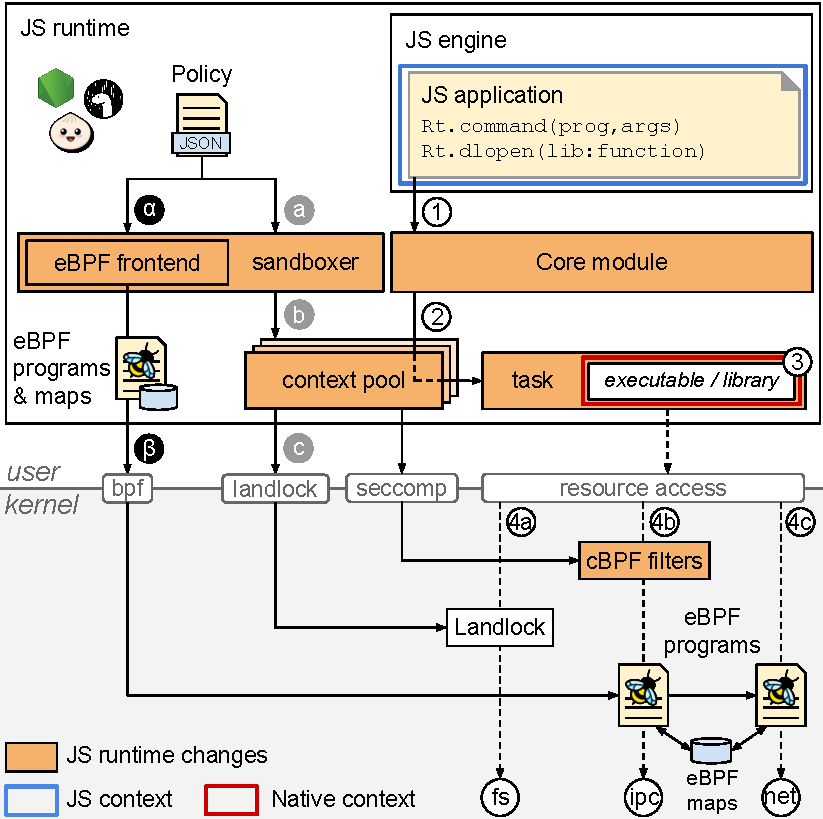
\includegraphics[width=\columnwidth]{chapters/natisand/fig/overview_sandbox}
  \caption[Integration of \natisand in JS runtimes]{
    Integration of \natisand in the JS runtime. Bootstrap: import
    security contexts ($\alpha$,~$\beta$), creation of the context
    pool ($a$,~$b$,~$c$). Application runtime: isolated execution of
    binary programs and shared library functions
    ($1$,~$2$,~$3$,~$4a$,~$4b$,~$4c$)
  }
  \label{fig:overview_sandbox}
\end{figure}
      
The architecture of our solution is shown in
Figure~\ref{fig:overview_sandbox}. Shortly after the JS runtime is
executed, \natisand parses the policy file input by the developer. Based on
the policy, a set of sandboxing and tracing programs
%
along with maps
%
are initialized and loaded into the kernel. A pool of isolated
contexts is also prepared by the sandbox. At runtime, \natisand intercepts
all the calls to native code performed by the application and executes
them safely in the proper isolated context.
%
A technical description of how our proposal is integrated into a
modern JS runtime is given in Section~\ref{subsect:arch}, while
details about its isolation features are reported in
Section~\ref{subsect:isolation}. The policy syntax used by \natisand to
configure permissions, along with the support to policy
generation, are described in Section~\ref{natisand:sect:policy}.


\subsection{Integration with JS runtimes}
\label{subsect:arch}

\natisand complements the architecture of the JS runtime with the addition
of the {\em sandboxer}, a component that parses the policy and
enforces the isolation of native code accordingly. In the following we
explain the operations performed by the runtime to use it, referring to Figure~\ref{fig:overview_sandbox}.

\paragraph{Bootstrap}
The JS runtime boot procedure is modified to read the JSON policy
file, which is then parsed by the sandboxer~\blackcircle{$\alpha$} to
retrieve the information associated with each security context. Based
on the policy,
%
  %
  the sandboxer (i) configures the required Seccomp filters, and (ii)
  prepares and loads into the kernel the necessary eBPF programs and
  maps~\blackcircle{$\beta$}. The eBPF programs are used to track the
  security contexts and enforce network-related and (part of)
  IPC-related restrictions (more details in
  Section~\ref{subsect:isolation}). Maps instead associate each
  isolated compartment with a security policy, and store the ambient
  rights granted to them. To determine which policy is associated with
  a given isolated compartment we leverage its kernel {\tt
    task\textunderscore struct} identifier, which is used as the key
  in an eBPF map of type {\tt TASK\textunderscore STORAGE} to lookup
  the policy identifier. This information is used as an address within
  an eBPF map of type {\tt ARRAY\textunderscore OF\textunderscore
    MAPS}, and permits to retrieve an inner {\tt HASH} map containing
  the ambient rights.
%
Loading eBPF maps and programs is a privileged operation
that requires the {\tt CAP\_BPF}, {\tt CAP\_PERFMON}, {\tt
  CAP\_NET\_ADMIN} capabilities to be performed, thus we grant the JS
runtime executable the corresponding Linux file
capabilities~\cite{file-based-capabilities}.  After the completion of
these steps, the capabilities are no longer necessary, hence they are
dropped. This satisfies the requirement that root permissions at
runtime are not needed for the activation of security contexts.

The sandboxer is also responsible for the creation of the security
contexts where native code will be executed at runtime. Each context
is an OS thread with permissions restricted by Landlock, Seccomp, and
eBPF. To avoid paying the performance cost to instantiate
each security context during the invocation of executables
and shared libraries, we modified the JS runtime to allocate
a thread per security context defined by the policy, restrict their
permissions, and then, park them in a context pool (\graycircle{a},
\graycircle{b}, \graycircle{c}).
%
  %
  With Landlock and Seccomp, restriction of privileges is performed
  calling the corresponding syscalls from the specific context, while
  restriction of permissions based on eBPF is simply performed
  invoking the uprobe {\tt attach\textunderscore policy} reported in
  Table~\ref{table:hooks}a. As a result, the {\tt task\textunderscore
    struct} identifier of a given context is annotated in the
  dedicated eBPF map along with the associated policy identifier.  
%
This design choice allows to reuse security contexts, thus
  minimizing latency, which, as highlighted in the objectives
(Section~\ref{subsect:objectives}), is a critical metric for web
applications.

\paragraph{Application runtime}
After the web application is started, two operations can lead to the
execution of native code: (i) the execution of a binary program in a
subprocess, and (ii) the invocation of a shared library. \natisand
intercepts all the requests originating from the web application that
require to execute native code~\whitecircle{1}, and leverages the
sandboxer to assign them to the proper pre-allocated isolated
context~\whitecircle{2}. Based on the type of request, a dedicated
task inheriting the selected security context is launched and
used to execute the native code~\whitecircle{3}.
Specifically, when there is a request to run an executable,
the JS runtime forks a process. On the other hand, when a shared
library should be loaded, a thread is spawned. The consequence is
that any request to access filesystem, IPC, and network resources will
be subject to the restrictions imposed by the LSMs
(\whitecircle{4a},~\whitecircle{4b},~\whitecircle{4c}). The approach
implemented by \natisand ensures that native code is never loaded nor
executed in a task running unconstrained, thus strengthening the
boundary between the web application and the OS.

\subsection{Isolation features}
\label{subsect:isolation}

Native code executed in isolated contexts can vary from library
functions to entire programs. In the following we detail how \natisand
enforces isolation and summarize the sandboxing features.

\paragraph{Policy inheritance}
While Landlock and Seccomp guarantee policy inheritance after a {\tt
  clone} syscall is performed, the eBPF map that tracks the
restricted contexts must be updated explicitly. To this end, \natisand
relies on the eBPF tracing programs that are loaded into the
kernel during the bootstrap phase and are attached to the {\tt fork}
and {\tt exit} tracepoints reported in
Table~\ref{table:hooks}a. Whenever a security context allocates a new
task with a fork operation, the tracing program registers
a new entry into the map of restricted contexts. The entry
  maps the task identifier of the child to the policy identifier
  associated with the parent. When instead a context terminates its
  duties and issues an exit, its task identifier is deleted from the
  map. No intervention by the developer is required, as policy
inheritance is transparently handled by our solution.

\paragraph{Filesystem}
\natisand restricts access to the filesystem using Landlock. The sandbox
enforces a straightforward {\tt read}, {\tt write}, {\tt exec} (RWX)
permission model, specified with three allow-list vectors (e.g., lines
5, 6, and 7 in Listing~\ref{natisand:lst:policy_file}). After the security
context has been activated, the available permissions can only be
further restricted.

\begin{table}[!t]
	\small
	\begin{tabular}{cc}
	  \parbox{0.47\columnwidth}{
      \centering
      \begin{tabular}{l}
        \toprule
        \multicolumn{1}{c}{\bf Context lifecycle} \\ \midrule
        {\tt uprobe\slash attach\textunderscore policy} \\
        {\tt tp\textunderscore btf\slash sched\textunderscore process\textunderscore fork} \\
        {\tt tp\textunderscore btf\slash sched\textunderscore process\textunderscore exit} \\
        \bottomrule
      \end{tabular}
	  } &
	  \parbox{0.47\columnwidth}{
      \centering
      \begin{tabular}{l | l}
        \toprule
        \multicolumn{2}{c}{\bf Access control}                  \\ \midrule
        \multirow{3}{*}{\rotatebox{90}{IPC}}      & {\tt fentry\slash fifo\_open}     \\
                                  & {\tt lsm\slash socket\_bind}      \\
                                  & {\tt lsm\slash socket\_connect}   \\ \midrule
        \multirow{3}{*}{\rotatebox{90}{Network}}  & {\tt lsm\slash socket\_bind}      \\
                                  & {\tt lsm\slash socket\_create}    \\
                                  & {\tt lsm\slash socket\_connect}   \\
        \bottomrule
      \end{tabular}
	  } \\
	  {\small\bf (a)} & {\small\bf (b)}
	\end{tabular}
	\caption{\label{table:hooks} Hooks and tracepoints monitored by
	  \natisand}
      \end{table}

\paragraph{IPC}
To explain the isolation features \natisand provides, we start with a
description of how programs and libraries generally use IPC.
Native programs often rely on parallelism and concurrency to achieve
high resource utilization. Parallel execution typically requires to
handle synchronization and communication between a parent and a group
of child tasks. In this setting, best practice suggests to provide the
children with the necessary communication channels through the
inheritance properties of the {\tt clone} syscall~\cite{doc-pipe}. For
instance, when two programs are piped in the Bash shell, an IPC
mechanism, in the form of a pipe, is created by the shell process and
is inherited by the two child programs, so that the latter can read
the output from the former. Similarly, a parent and a child task can
leverage an unnamed UNIX socket pair to share
messages~\cite{doc-socketpair}. These use cases do not pose a
significant security risk, since (i) the communication happens between
tasks associated with the same security context, and (ii) the IPC
channels used to communicate are not visible to other services running
on the host OS. Conversely, CVE-2020-16125 and CVE-2021-3560
demonstrate that uncontrolled interaction with globally available IPC
channels used by other services can lead to concrete security
problems.

To block the communication between components associated with
incompatible security contexts, \natisand by default denies IPC over
globally visible communication mechanisms. In this category there are
fifo (i.e., named pipes), message queues, named semaphores,
non-private shared memory, signals, and UNIX named sockets.  Many of
these mechanisms can be fully blocked by denying access to the related
system calls, but in some cases the evaluation of syscall
configuration flags is necessary. For instance, the creation of shared
memory maps is permitted by the sandbox only when the {\tt mmap}
syscall is invoked with {\tt MAP\_ANONYMOUS} or {\tt
  MAP\_PRIVATE}. Similarly, the creation of named special files is
allowed only when the {\tt mknod} and {\tt mknodat} syscalls are not
invoked with {\tt S\_IFIFO} and {\tt S\_IFSOCK}. Syscall filtering
based on configuration flags is performed efficiently by \natisand using
Seccomp.
However, the information available to Seccomp is not always sufficient
to make the access decision. This is the case for the {\tt bind}, {\tt
  connect}, {\tt open}, and {\tt openat} syscalls.  Indeed,
information about the type of socket referenced for the {\tt bind} and
{\tt connect} syscalls resides in user memory, and unfortunately
Seccomp cannot safely dereference it (due to
TOCTOU risks~\cite{seccomp-toctou}). Likewise, the {\tt open} and {\tt openat} syscalls do
not represent the type of file to be opened through configuration
flags, so Seccomp cannot handle the specific case properly. To solve
these problems \natisand relies on the eBPF programs attached to the hooks
reported in Table~\ref{table:hooks}b (which are not affected by TOCTOU
issues, since they operate on arguments that were previously deep
  copied by the kernel). In particular, in the case of UNIX sockets the programs are
attached to the {\tt lsm/socket\_bind} and {\tt lsm/socket\_connect}
hooks, while for fifo files the kernel function {\tt fifo\_open} is
used. A summary of the IPC mechanisms controlled by \natisand, along with
the LSMs leveraged to perform the security checks, is reported in
Table~\ref{table:ipc}.

\paragraph{Network}
%
\natisand permits to control how each isolated context connects to network
resources. In detail, it permits to completely revoke access to the
network, to connect only to a restricted list of hosts, and when
needed, to use the network without restrictions. The sandboxer relies
on eBPF programs to enforce permissions. The programs restrict the
ability to {\tt create}, {\tt connect}, and {\tt bind} sockets, and
are thereby attached to the LSM hooks reported in
Table~\ref{table:hooks}b.

The creation of a socket opens a communication channel and returns a
file descriptor as a result. By default, the sandboxer restricts the
available communication domains to Internet Protocol (IP), denying
applications the use of protocol families such as Bluetooth, Radio,
VSOCK, and many more (this information is directly available
  from the arguments input to the {\tt socket\textunderscore create}
  interface). No restrictions are instead applied to UNIX domain
sockets and the type of socket to be opened (e.g., stream,
datagram). Opening a connection to a host is permitted only when the
developer grants the isolated context to do so. The eBPF
program that checks the opening of a connection first
  recovers the policy restricting the current security context, then
  uses it as a key to lookup the map of ambient rights from the {\tt
    ARRAY\textunderscore OF\textunderscore MAPS} described in
  Section~\ref{subsect:arch}. The ambient rights map is an allow-list
  that stores the reachable (i.e., policy allowed) hosts, hence the
  security check is carried out with a lookup. Each network resource
is uniquely identified by its IP address and port. Internally,
we use the value zero for the port to represent the
  permission of opening a connection to a given host on every port.

Up to now, we have discussed the restrictions when
the application connects as a client to a service. However, web
applications frequently need to serve incoming requests. To do so, it
is necessary to assign a ``name'' to a socket -- i.e., configuring its
address. This operation is done with the {\tt bind} syscall,
  and we decided to permit it only when the policy 
  gives the current security context access to the corresponding
address and port pair. Again, the value zero for the port is used as a
placeholder to allow binding on every port. On the other hand, no
restrictions are applied to the {\tt listen} and {\tt accept}
syscalls. Listen only marks a socket as passive, meaning that it will
be used to accept incoming requests. However, no connection to a
socket can happen if an address was not previously assigned to
it~\cite{doc-listen}.  The same applies to {\tt accept}, which is used
to extract the first connection request from the queue of pending
connections~\cite{doc-accept}.

\begin{table}[t!]
\centering
\small	
\setlength{\tabcolsep}{0.06cm}
\begin{tabular}{| l | l | l | c | c |}
  \hline
  {\bf IPC} & {\bf Subclass} & {\bf Linux system call} & {\bf Seccomp} & {\bf eBPF} \\ \hline
  \multirow{3}{*}{\shortstack[l]{Message \\ queue}}  & \multirow{2}{*}{POSIX}     & mq\_open, mq\_getsetattr, mq\_notify,     & \multirow{2}{*}{\cmark} & \\
            &                            & mq\_timedreceive, mq\_timedsend, mq\_unlink           &                         & \\ \cline{2-5}
            & System V                   & msgctl, msgget, msgrcv, msgsnd            & \cmark                  & \\ \hline
  Pipe      & Named                      & mknod, mknodat, open, openat              & \hspace{0.1cm}\cmark*                 & \cmark \\ \hline
  \multirow{2}{*}{Semaphore}                         & POSIX                      & futex, mmap                               & \hspace{0.1cm}\cmark*                 & \\ \cline{2-5}
            & System V	& semctl, semget, semop, semtimedop         & \cmark                  & \\ \hline
  \multirow{2}{*}{\shortstack[l]{Shared \\ memory}}  & POSIX                      & mmap                                      & \hspace{0.1cm}\cmark*                 & \\ \cline{2-5}
            & System V                   & shmat, shmctl, shmdt, shmget              & \cmark                  & \\ \hline
  \multirow{2}{*}{Signal}                            & Standard  & kill, pidfd\_send\_signal, tgkill, tkill  & \cmark                  & \\ \cline{2-5}
            & Real-time & rt\_sigqueueinfo, rt\_tgsigqueueinfo      & \cmark                  & \\ \hline
  UNIX socket    & Named                      & bind, connect, mknod, mknodat             & \cmark*                 & \cmark \\ \hline
\end{tabular}
\caption[LSMs used by \natisand to restrict Linux IPC]{
  LSMs used by \natisand to restrict Linux IPC. The checkmark
  \cmark* indicates when Seccomp needs to evaluate the syscall
  configuration flags to make the access decision
}
\label{table:ipc}
\end{table}

  \paragraph{Limitations}
  %
  While \natisand significantly restricts the set of permissions and system
  resources associated with subprocesses and shared libraries, it
  provides strong memory isolation guarantees only when executables
  are run, as each subprocess is executed within its own address
  space. On the other hand, shared libraries are loaded within the
  hosting thread address space, hence a native library bug can impact
  the web application memory. Several research works have studied this
  problem and have proposed countermeasures~\cite{RLBox,
    kirth2022pkru, wu2012codejail, cali, vasilakis2018breakapp,
    binwrap}. In general, these works are compatible with the design
  of our solution, therefore they could be used in conjuction with
  \natisand to improve isolation of shared libraries. Among them,
  BreakApp~\cite{vasilakis2018breakapp} and BinWrap~\cite{binwrap}
  propose approaches tailored for interpreted languages, but they
  require either the introduction of wrappers or the execution of
  remote procedure calls. RLBox~\cite{RLBox} provides strong
  guarantees against memory corruption, but it demands the developer
  to manually retrofit existing code, a process that can take up to
  ``few days'' for each library according to the authors. Improved
  intra-process isolation can also be achieved leveraging dedicated
  hardware features like Intel Protection Keys for Userspace (PKU),
  but as demonstrated by PKU Pitfalls~\cite{pku-pitfalls} these
  solutions can be bypassed using kernel functions that are agnostic
  of intra-process isolation (i.e., the attacks use the kernel as a
  confused deputy). Since \natisand is completely aligned with the memory
  isolation assumptions made by the kernel, our solution is not
  affected by this issue.  




%%% Local Variables:
%%% mode: latex
%%% TeX-master: "../main.tex"
%%% End:

\section{Policy}
\label{natisand:sect:policy}

In this section we present the structure of the policy file, then we
explain how to generate the permission rules.

\subsection{Policy structure}
\label{sect:sci-ffi-policy-structure}

JS applications executed by \natisand are associated with a policy
file. The policy must be provided by the developer before the
application is run, and to this end, a CLI flag (e.g., {\tt
  native-sandbox}) needs to be added to the JS runtime. The policy
file is formatted in JSON, with the following structure: a policy
defines an array of objects and each object details the permissions
available to a security context.  Within each object, a {\em name} is
used to identify the context, a {\em type} indicates whether the
context applies to an executable, a library, or a function of a
library; the sections {\em fs}, {\em ipc} and {\em net} are used to
configure the corresponding permissions. The structure of the objects
is flexible, and only a {\em name} is required to configure a valid
context. As the policy follows a {\em default-deny} model, a context
that specifies only its name has no permissions at runtime. An excerpt
from a policy file is shown in Listing~\ref{natisand:lst:policy_file} (the
complete example is reported in Appendix~\ref{appendix:curl_policy}),
while a summary of the most relevant policy features is described
next.

\subsubsection*{Name, Type}

The name and type elements are used by \natisand to determine which policy
context must be enforced. The type element can be set to {\tt
  executable} (the default value), {\tt library} or {\tt function}.
At runtime \natisand extracts the absolute path of the native program and function
name, and based on the information available, it identifies the most
selective entry in the policy. This gives the developer the
flexibility to use different policies in case binaries and libraries
have the same basename, or when different functions
from the same library are invoked. Moreover, since absolute
paths are used, this approach ensures symlinks cannot trick the lookup
of the security context. Listing~\ref{natisand:lst:policy_file} shows
a policy that is enforced every time the application runs the curl
program.

\subsubsection*{Fs}

The fs element is used to configure filesystem-related permissions. Fs
stores three optional arrays: {\em read}, {\em write} and {\em
  exec}. Filesystem paths are used as array values. As an example, the
context detailed in Listing~\ref{natisand:lst:policy_file} can read and execute
the curl binary, and write to {\tt response.json} in the current
working directory of the web application. In case the developer wants
to operate with a coarser granularity, the value {\tt true} can be
used to replace any of the {\em fs}, {\em read}, {\em write} and {\em
  exec} arrays to grant access to the whole filesystem.

\subsubsection*{Ipc}

To restrict IPC access we decided to expose developers a simple
interface where flags can be turned on and off based on their needs.
Six optional flags are available in the policy: {\em fifo}, {\em
  message}, {\em semaphore}, {\em shmem}, {\em signal}, and {\em
  socket}. For example, in Listing~\ref{natisand:lst:policy_file}, curl is
allowed to use abstract, named, and unnamed Unix sockets. It is up to our sandboxer to abstract away the complexity
of the underlying architecture and enforce the policy when IPC is
performed between groups of threads associated with separate
contexts. No understanding of the standards available (e.g., System V,
POSIX) is required by developers to restrict the permissions
associated with their application. Similarly to the filesystem case, the
developer can use a coarser granularity by setting the {\em ipc}
element to {\tt true}, enabling all communication mechanisms.
Notice that globally available IPC channels are often bound to
filesystem resources, so, while the granularity of the six flags
described above may seem coarse, finer-grained permissions can be
specified leveraging the path associated with the IPC resource.
For example, the developer can restrict the use of a specific named
pipe (pinned to the filesystem) by using its fully qualified path.

\subsubsection*{Net}

Web application developers are often interested in restricting the
hosts an application can connect to. The policy permits to
specify an array of reachable hosts. Each host is fully qualified by
its URL/IP, and the sequence of permitted ports. As in the case of the
filesystem, the policy permits to grant access to the network without
limitations (setting {\em net} to {\tt true}), enable all the ports
for a specific host (setting {\em ports} to {\tt true}), or completely
remove access to the network (leveraging the default-deny
behavior). In Listing~\ref{natisand:lst:policy_file}, the process executing
curl is only allowed to connect to {\tt https://www.example.com} on
port 443.

\begin{lstlisting}[
    abovecaptionskip=-5pt,
    caption=Example of JSON policy file with single context,
    float=tp,
    floatplacement=tbp,
    language=json,
    label=natisand:lst:policy_file,
]
[{
   "name": "/usr/bin/curl",
   "type": "executable",
   "fs": {
           "read":   ["/usr/bin/curl", ...],
           "write":  ["response.json"],
           "exec":   ["/usr/bin/curl", ...]
   },
   "ipc": {
           "socket": true,
   },
   "net": [{
	   "name":   "https://www.example.com",
	   "ports":  [443]
   }]
}]
\end{lstlisting}


\subsection{Policy generation}
\label{sect:sci-ffi-policy-generation}

While designing \natisand we opted for a minimal and easy to understand
policy syntax to target a broad spectrum of users. However, writing a
policy for large components may be a tedious and tricky task, since we
do not expect all the developers to be aware of how binaries and
external libraries used by their web application work internally. To
assist the developer, we follow an approach similar to
SlimToolkit~\cite{slimtoolkit}, where a service is run against a test
suite to generate the security profile.
Specifically, we developed a CLI utility written in Go that provides
generation of policy templates the developer can understand,
modify, and audit. The utility persists policy-relevant information
in a SQLite database, and exposes to the user many functions that
permit to configure multiple contexts, merge the results collected
from multiple tests, and refine policies interactively.
In the following we provide details on
the work we performed for each of the protected subsystems.

\subsubsection*{Filesystem}

The automatic retrieval of the dependencies of a binary is a
well-known problem. Our utility is capable to discover the
dependencies of programs installed as ELF files, and programs that are
spawned by dedicated POSIX or shell wrappers. The utility first uses
{\em ldd}~\cite{linux-ldd} to discover the direct and transient
dependencies, then, it relies on {\em strace}~\cite{linux-strace} to
monitor the interaction between the kernel and a traced binary, so to
complement the information previously found with additional
filesystem permissions.

\subsubsection*{IPC}

\natisand adopts a policy language that abstracts away IPC complexity.  Our
utility supports policy generation by analyzing the results of
multiple test cases where the Seccomp filter and eBPF
programs of the sandboxer are set to {\em auditing mode}.  These
programs return the flags to be enabled.

\subsubsection*{Network}

Network rules are relatively easy to write. However, we do not
assume developers to be necessarily aware of every network connection
needed by the native code. So, we automate the generation of the
policy by observing the execution of the binary with eBPF programs.
In fact, these provide a list of the domain names resolved, their IPs,
and those hardcoded IPs the utility connects to without performing
name resolution. To track domain name resolutions we attach a {\tt 
  uprobe} to the {\tt getaddrinfo} function of the libc library,
for IPs we observe network socket connections using {\tt kprobes} on
{\tt socket\_bind} and {\tt socket\_connect} LSM hooks.
%
 To handle IP address migrations that may occur at runtime,
  we similarly propose to capture the list of IPs returned by the {\tt
    getaddrinfo} with a dedicated eBPF program, which also updates the
  eBPF map of allowed hosts accordingly. By doing so we make sure that
  the security checks reflect the policy. This approach can also be
  extended monitorng DNS traffic on port 53, hence providing support
  for native components that do not rely on libc functions.  

\vspace{2 mm}
\noindent Policy generation is subject to limitations: (i) policy
generation for malicious code 
produces overly permissive policy and obviously cannot be trusted,
(ii) test suite with limited coverage might provide overly strict
policies not allowing the execution of legitimate code.
Overall, the correctness of the policy depends on the test suite used
to collect the permissions. The closer the tests align with the use of
the native utility in production, the more the developer can consider
the policy generated effective. Nonetheless, to have complete
assurance that the policy generated is correct, an auditing process
may be required.

%%% Local Variables:
%%% mode: latex
%%% TeX-master: "../main.tex"
%%% End:

\section{Case study: Deno runtime}
\label{sect:case-study-deno}

There are three well-known alternatives for the execution of JS code
on the backend, namely Node.js, Deno, and Bun. As highlighted in
Section~\ref{sect:background-js-runtime}, their architectures have
strong similarities, and NatiSand is designed to be compatible with
all of them (since no assumption is made on specific runtime
components). Nevertheless the integration is not trivial, and it requires
significant engineering effort, therefore we integrated \natisand into only
one of them to demonstrate the achievement of the set objectives
(Section~\ref{subsect:objectives}). In this section we explain our
decision, then we highlight the main architectural changes.

\subsection{Runtime selection}
\label{sect:deno-selection}

Considering (i)~popularity among web developers, (ii)~availability and
support of third-party modules, and (iii)~security-oriented features
provided by the runtime, we selected Deno. Bun is still in beta
version (v0.5.8), so it is the least used by developers.
Node.js is nowadays the most
widely used platform, and it offers developers the largest collection
of open source packages. However, Node.js by default does not prevent
JS applications to access system resources, and although it
recently introduced a module-based permission model, the feature is
experimental~\cite{node-permissions}. Deno was instead designed with the protection of
the host as one of its main goals~\cite{nodejs-regret}, thus no access to privileged system
resources is given to JS applications unless the developer
explicitly grants it. Deno provides the
{\em Node Compatibility Mode}~\cite{deno-compatibility-mode}, a
feature enabling the reuse of
code and libraries originally built for Node.js. The availability of
this function permits to
import packages hosted by Deno on {\tt deno.land/x}, as well as
modules published to npm. To conclude, Node.js and Deno prevail
over Bun on all three dimensions. Node.js wins over Deno on
popularity (but Deno is quickly growing), they are comparable in terms
of third-party modules, and Deno significantly outperforms Node.js on
security oriented-features, leading us to choose Deno.

\subsection{Deno integration}
\label{subsect:deno-integration}

Deno has a modular architecture organized into components. Three of
them are particularly important for \natisand: (i) {\em
  rusty\textunderscore v8}, the package that bridges Deno and the V8
engine implementing the set of bindings to the V8's C++ API, (ii) {\em
  deno\textunderscore core}, which leverages {\em rusty\textunderscore
  v8} to expose the interfaces provided by Deno to the JS application,
and (iii) {\em deno}, which defines the runtime executable together
with the Command Line Interface.

\paragraph{Bootstrap}
%
Shortly after the Deno executable is run, the {\em deno} component is
used to read the permissions granted by the developer via CLI. We
extended this stage to read and parse the policy file specified with
the new {\tt native-sandbox} flag, then we added the permissions
associated with each security context to the {\em global state} stored
by the runtime. To complete the bootstrap phase, we also integrated
the steps to load the necessary eBPF programs and to initialize the
pool of isolated contexts, as explained in Section~\ref{subsect:arch}.

\paragraph{Application runtime}
%
After the JS application is started, the function
calls that cannot be directly handled by V8 are routed to the Deno
runtime through the bindings defined by {\em rusty\textunderscore
  v8}. Each of them is associated with the {\em op\textunderscore
  code}, a unique code identifying the operation to be
performed. The {\em deno\textunderscore core} component receives such
requests, it checks the permissions available from the global state,
and serves them accordingly. We identified requests that
require to execute native code (e.g., {\tt command}, {\tt dlopen},
{\tt run}), and modified {\em deno\textunderscore core} so that they
are restricted by \natisand. The {\em op\textunderscore code} along
with the arguments are used to select the proper security context.


\subsection{Support to fast JS calls}
\label{subsect:fast-api}

In October 2020 V8 announced the support to fast JS
calls~\cite{v8-fast-calls}. The function allows V8 to directly invoke optimized native
functions without leveraging the bindings that connect V8 and the
embedder (e.g., JS runtime). This permits to obtain substantial
performance gains, since native function calls can be resolved in
nanoseconds. 

Deno has introduced unstable support to fast JS calls in July
2022~\cite{deno-v1234}. The change affected the implementation of the
{\em dlopen} API, which is now able to generate an optimized and a
fallback (i.e., standard) execution path for native functions. The
optimized path is triggered only when V8 is actually able to optimize
a symbol, and it entails the execution of code leveraging the fast
call interface. While the optimized path is associated with minimum
overhead, from a security perspective it permits the web application
to execute native code without the mediation of the JS runtime,
invalidating the security reference monitor of Deno.
%
In our prototype we address this Deno security issue offering
developers two alternatives: (i) turn off
the fast call support and safely rely on the execution of sandboxed
native functions with \natisand without any code change, and (ii) enable insecure fast calls but
allow to select the JS functions that need to be isolated with minimal code changes. The second
option permits to take advantage of fast calls when performance is
critical and risks are limited (e.g., arithmetic operations), and at
the same time benefit from the security features \natisand provides. To
this end, we introduced a new API named {\tt Deno.nativeCall()}. The API receives, as first argument, the name of the function
to be sandboxed, along with the list of its arguments.
Listing~\ref{lst:sqlite3_example} shows how to sandbox the functions
from the native database driver {\em sqlite3}.
%
\begin{lstlisting}[
	abovecaptionskip=-5pt,
	caption=Code sandboxing with {\tt nativeCall()},
	float=t,
	floatplacement=tbp,
	label=lst:sqlite3_example,
	language=javascript,
	]
function query(db, stmt) {
    const sqliteDB = new sqlite3.Database(db);
    const query = sqliteDB.prepare(stmt);
    const tuples = query.all();
    sqlite_db.close();
    return tuples;
}

const db = "database.db";  
const stmt = "SELECT * FROM table";
const ts = Deno.nativeCall(query, [db, stmt]);
console.log(ts); // print tuples
\end{lstlisting}

%%% Local Variables:
%%% mode: latex
%%% TeX-master: "../main.tex"
%%% End:

\section{Experiments}
\label{natisand:sect:exp}

\pap must satisfy two properties to be practical: (i) it must mitigate
real-world vulnerabilities by blocking the associated exploits, and
(ii) it must introduce a limited overhead compared to a scenario where
no protection is applied. In the experimental evaluation, we first
show our solution is able to protect web applications relying on
binary programs and shared libraries affected by high severity
vulnerabilities (Section~\ref{subnatisand:sect:exploit-mitigation}), then we
investigate the performance of our approach
(Section~\ref{subsect:performance-eval}).
Both tests use a server with Ubuntu 22.04 LTS, an AMD Ryzen 3900X CPU,
64 GB RAM, and 2 TB SSD.

\subsection{Exploit mitigation}
\label{subnatisand:sect:exploit-mitigation}

To conduct our analysis we built a representative sample of
vulnerabilities targeting executables and libraries widely used in web
applications. We identified the 32 CVEs reported in
Table~\ref{table-cve}. The entries are separated into three classes:
Arbitrary Code Execution (ACE), Arbitrary File Overwrite (AFO), and
Local File Inclusion (LFI). The list of vulnerable utilities includes
programs used to compress files (e.g., GNU Tar, RAR, Zip), to process
multimedia (e.g., FFmpeg, GraphicsMagick, ImageMagick), database
drivers (e.g., SQLite), and also Machine Learning libraries (e.g.,
Lightning, Sockeye, TensorFlow). We highlight that the vulnerabilities
affect popular open source modules with 2.6M downloads/week available
from the npm and {\tt deno.land/x} archives. Concrete examples are
sharp and fluent-ffmpeg from npm, or flat and sqlite from {\tt
  deno.land/x}.

\begin{table}[!t]
	\setlength{\tabcolsep}{3mm}
	\begin{tabular*}{\columnwidth}{ l l l l l}
	  \toprule
	  {\bf Class} & {\bf CVE Id} & {\bf Utility} & {\bf Type} & {\bf Use case}\\
          \midrule
	  \multirow{25}{*}{ACE}                     & CVE-2016–3714    & ImageMagick    & bin & Image processing    \\
						    & CVE-2019-5063    & OpenCV         & lib & Computer Vision     \\
						    & CVE-2019-5064    & OpenCV         & lib & Computer Vision     \\
						    & CVE-2020-6016    & GNSockets      & lib & P2P networking      \\ 
						    & CVE-2020-6017    & GNSockets      & lib & P2P networking      \\ 
						    & CVE-2020-6018    & GNSockets      & lib & P2P networking      \\
						    & CVE-2020-17541   & libjpeg-turbo  & lib & Compress image      \\
						    & CVE-2020-24020   & FFmpeg         & lib & Video processing    \\
						    & CVE-2020-24995   & FFmpeg         & lib & Video processing    \\
						    & CVE-2020-29599   & ImageMagick    & bin & Image processing    \\
						    & CVE-2021-3246    & libsndfile     & lib & Audio encoding      \\
						    & CVE-2021-3781    & Ghostscript    & bin & PDF processing      \\
							& CVE-2021-4118    & Lightning      & lib & Machine learning    \\
						    & CVE-2021-20227   & SQLite         & lib & Query database      \\
						    & CVE-2021-21300   & Git            & bin & Clone repository    \\
						    & CVE-2021-22204   & ExifTool       & bin & Extract metadata    \\
						    & CVE-2021-37678   & TensorFlow     & lib & Machine learning    \\
							& CVE-2021-43811   & Sockeye        & lib & Translation         \\
						    & CVE-2022-0529    & Unzip          & bin & Decompress archive  \\
						    & CVE-2022-0530    & Unzip          & bin & Decompress archive  \\
							& CVE-2022-0845    & Lightning      & lib & Machine learning    \\
						    & CVE-2022-1292    & OpenSSL        & bin & Verify certificate  \\
						    & CVE-2022-2068    & OpenSSL        & bin & Verify certificate  \\
						    & CVE-2022-2274    & OpenSSL        & lib & Cryptography        \\
						    & CVE-2022-2566    & FFmpeg         & bin & Video processing    \\
	  \midrule
	  \multirow{4}{*}{AFO}  & CVE-2016-6321    & GNU Tar        & bin & Decompress archive  \\
							& CVE-2017-1000472 & POCO           & lib & Common libraries    \\
						    & CVE-2019-20916   & Pip            & bin & Dependency fetch    \\
						    & CVE-2022-30333   & UnRAR          & bin & Decompress archive  \\
	  \midrule
	  \multirow{3}{*}{LFI}  & CVE-2016-1897    & FFmpeg         & bin & Video processing    \\
						    & CVE-2016-1898    & FFmpeg         & bin & Video processing    \\
						    & CVE-2019-12921   & GraphicsMagick & bin & Image processing    \\
	  \bottomrule
	\end{tabular*}
	\caption{\label{table-cve} Sample of CVEs mitigated by \pap}
\end{table}


First, we checked that public Proofs of Concept of the CVEs in
Table~\ref{table-cve} successfully exploit the vulnerable version of
the utilities. Then, we analyzed whether the vulnerabilities were
exploitable sending the malicious payload through the JS module
interface, and confirmed the feasibility of the attack. The {\em Node
  compatibility mode} was leveraged to execute in Deno the modules
downloaded from npm. We finally repeated the experiment activating the
security functions provided by \pap, and verified that the attack was
no longer successful, while the application was still able to serve
benign requests (i.e., no functionality loss). The only change we
introduced in the experiment was the specification of a security
policy through the {\tt native-sandbox} CLI argument. The policy was
generated using the tool described in
Section~\ref{sect:sci-ffi-policy-generation}. No modification to the
web application, nor its dependencies, was required to benefit from
the new sandboxing capabilities.


From a security perspective it is worth mentioning that \pap can
mitigate attacks at multiple levels. For instance, in CVE-2022-2566 a
heap out-of-bound memory bug exists in FFmpeg. The goal of the
attacker is to achieve Arbitrary Code Execution sending to the web
application a malicious {\tt MP4} payload. \pap denies the compromised
component attempts to access confidential files, open reverse shells,
interact with privileged services through IPC, and transfer data to
unauthorized network hosts. We point out that, while sandboxing limits
the privileges an attacker can gain from exploiting a vulnerable
program, it cannot eliminate vulnerabilities, nor it can
make infeasible to use them in an exploit chain.


\subsection{Performance evaluation}
\label{subsect:performance-eval}

To assess the performance of \pap we considered a broad set of
programs, including several GNU Core Utilities, executables to process
multimedia, database drivers, and Object Character Recognition
engines. The goal is twofold: (i) evaluate the slowdown compared to a
scenario where no protection is available (i.e., regular Deno), and
(ii) compare \pap with well known sandboxing and isolation frameworks.
In the following we first investigate the impact on executables, then
we analyze libraries.

\subsubsection{Executables}

In the first batch of experiments we analyze the overhead associated
with executables. Compared to the default scenario where no protection
is available, \pap spawns each program in a dedicated subprocess with
its own set of constrained ambient rights. A handful of
general purpose sandboxers can be adopted to achieve a comparable
degree of protection by wrapping the execution of each subprocess with the chosen sandboxing utility. In our evaluation, we considered {\em
  Minijail}~\cite{minijail} and {\em Sandbox2}~\cite{sandbox2}.
Minijail is a tool used in ChromeOS and Android to launch and sandbox
other programs based on the set of arguments specified, while Sandbox2
is a C++ library written by Google that can be used to sandbox entire
programs or portions of them. Both Minijail and Sandbox2 support
multiple containment techniques, such as the introduction of dedicated
user ids, restriction of the Linux capabilities, introduction of
policy-based Seccomp filters, and isolation based on Linux namespaces.

\paragraph{Benchmark I}
%
In the first benchmark we implemented a JS application to test the
execution of 17 common Linux utilities with
four configurations: Deno, \pap, Minijail, and Sandbox2. The
application uses {\tt Deno.run()} to spawn each utility in a
subprocess, and it leverages {\tt Deno.bench()} to determine the duration of each request. The
function ensures that each measure is statistically robust, as it
automatically performs a dynamic number of rounds based on the
duration of the test (i.e., the shorter the test duration, the higher
the number of repetitions). The results are shown in
Table~\ref{table:common-linux-utils} (tests are ordered by increasing
execution time). As expected, the cost of activating the sandbox is
amortized with the increase in the test duration. The tests also show
that \pap suffers from a smaller performance degradation compared to
Minijail and Sandbox2. This aspect is particularly evident for
short-lived utilities. The reason is that our approach is integrated
by design and, contrary to the other solutions, leverages lightweight
technologies that introduce a smaller performance footprint.

\begin{table}[!t]
	\centering
    \setlength{\tabcolsep}{3mm}
	\begin{tabular*}{0.8\columnwidth}{l r r r r r}
		\toprule
		{\bf Utility} & {\bf Deno \scriptsize{[ms]}} & {\bf Minijail} & {\bf Sandbox2} & {\bf \pap}\\
		\midrule
		b2sum   & 2.37      & 7.19x     & 9.37x & \bf{2.88x}    \\
		cut     & 2.52      & 7.11x     & 8.97x & \bf{2.86x}    \\
		sum     & 2.61      & 7.00x     & 8.25x & \bf{2.87x}    \\
		tac     & 2.76      & 6.51x     & 8.21x & \bf{2.34x}    \\
		wc      & 2.97      & 6.25x     & 7.69x & \bf{2.44x}    \\
		dd      & 3.60      & 5.29x     & 6.26x & \bf{2.23x}    \\
		seq     & 3.80      & 5.02x     & 5.96x & \bf{2.13x}    \\
		shuf    & 4.29      & 4.68x     & 5.55x & \bf{2.17x}    \\
		ls      & 4.75      & 3.72x     & 4.68x & \bf{1.76x}    \\
		factor  & 5.03      & 4.06x     & 5.03x & \bf{1.86x}    \\
		join    & 5.20      & 4.08x     & 5.18x & \bf{2.05x}    \\
		head    & 6.73      & 3.16x     & 3.85x & \bf{1.56x}    \\
		ping    & 12.20     & 2.27x     & 2.79x & \bf{1.47x}    \\
		sort    & 14.37     & 1.44x     & 1.77x & \bf{1.43x}    \\
		dig     & 22.14     & 1.71x     & 2.15x & \bf{1.17x}    \\
		wget    & 53.24     & 1.18x     & 1.42x & \bf{1.13x}    \\
		curl    & 81.27     & 1.23x     & 1.24x & \bf{1.16x}    \\
		\bottomrule
	\end{tabular*}
	\caption{\label{table:common-linux-utils} Average execution time
	  for common Linux utilities}
\end{table}
%
\begin{figure}[!t]
	\begin{subfigure}{0.48\columnwidth}
		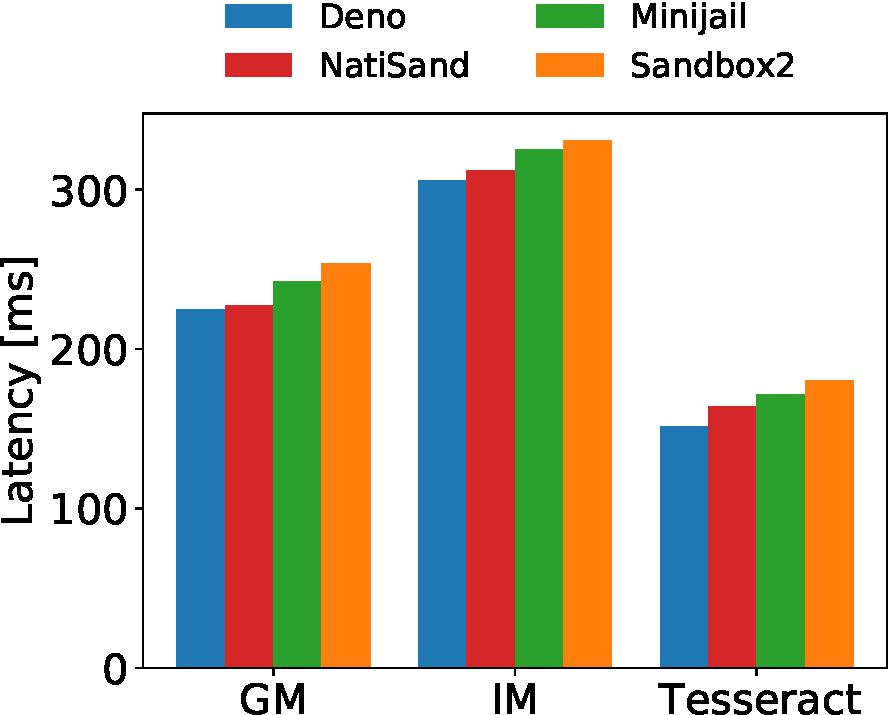
\includegraphics[width=\columnwidth]{chapters/natisand/fig/cropped-summary-subprocess-latency}
	\end{subfigure}%
	\hspace{0.5em}
	\begin{subfigure}{0.48\columnwidth}
		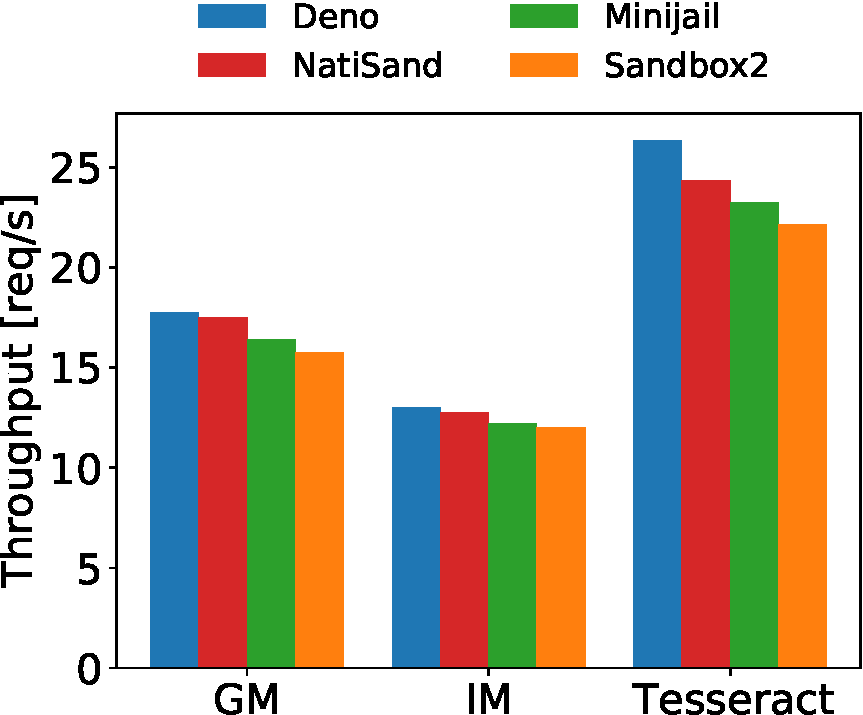
\includegraphics[width=\columnwidth]{chapters/natisand/fig/cropped-summary-subprocess-throughput}
	\end{subfigure}
	\caption[{Average latency and throughput of subprocess-based
	  microservices}]{
	  Average latency and throughput for microservices that execute
	  subprocesses
	}
	\label{fig:subprocess-lat-through}

\end{figure}

\paragraph{Benchmark II}
%
While the experiments part of Benchmark I focus on the server side
scenario, with Benchmark II we wanted to show the overhead experienced
by a remote client. To this end, we used three microservices,
each representing a real use case scenario of high performance native
programs. Two microservices rely on GraphicsMagick and ImageMagick, to
perform a {\em sharpen} operation on images input by the client, while
the third microservice relies on Tesseract to perform Optical
Character Recognition on a second sequence of images input by the
client. Similarly to the previous case, the test was repeated for each
of the four configurations: Deno, \pap, Minijail, and Sandbox2. This
time the HTTP benchmarking tool {\em wrk} was used to measure the
performance of each microservice.  Network bandwidth and latency are 1
Gbps and 10 ms, respectively, while 100 warmup requests were carried
out. Figure~\ref{fig:subprocess-lat-through} shows the average latency
and the throughput observed over a period of 30 seconds. The results
once again confirm the previous analysis, as longer durations make the
cost to setup the native sandbox less relevant. It is worth to mention
that \pap exhibits lower overhead compared to Minijail and Sandbox2,
with approximately 5 to 10 ms less latency for each microservice.


\paragraph{Usability}
%
Although general purpose sandboxers can be used to restrict the
permissions associated with executables, to provide a protection
comparable to \pap: (i) they force the developer to introduce changes in
the web application, and (ii) they require to understand in depth the
techniques used by the kernel to restrict ambient rights (e.g.,
capabilities, namespaces, Seccomp filters). Another problem is that to
restrict IPC and network with Minijail and Sandbox2 it is necessary to
leverage namespaces, which are characterized by coarser granularity
than \pap policies.



\subsubsection{Libraries}

In the second batch of experiments we analyze the overhead associated
with libraries. Contrary to the default JS runtime behavior, \pap
transparently executes native library functions in dedicated contexts
with limited ambient rights. A modern, valuable alternative approach
to isolate libraries is to compile them to WebAssembly (Wasm), a
standardized, portable binary instruction format executed in a memory
safe, sandboxed environment. This approach has gained considerable
attention recently, as browsers such as Firefox have used it to
retrofit some of their components to safely interface with native
libraries~\cite{RLBox}.

\paragraph{Benchmark III}
%
Similarly to Benchmark I, we implemented a JS application to highlight
the overhead experienced on the server when native libraries are
executed. In this case three configurations are evaluated: Deno, \pap,
and Wasm. The application tests the operations provided by four
popular libraries: (i) libxml2, to open and query XML data, (ii) libpng, to read metadata information and verify the
signature of a png image, (iii) opus to encode and create an audio
trace, and (iv) sqlite3, to open and query the Northwind
database. Test durations were again measured with {\tt Deno.bench()},
and the results are reported in
Table~\ref{table:native-lib-overhead}. Deno
exhibits a consistent performance advantage for operations that
require up to 30 microseconds. However, \pap proves to be more
efficient than Wasm, which in turn is affected by a substantial
overhead in almost every test. This difference is due to the nature of
Wasm; while there have been improvements, the just-in-time
compiled language~\cite{wasm-compilation-pipeline}
remains slower than its native counterpart. Remarkable are the cases
of opus and sqlite3, which used {\tt nativeCall} and demonstrate its
efficiency.

\paragraph{Benchmark IV}
%
To understand the slowdown perceived by a remote client, we exposed
the functions of the libpng, opus, and sqlite3 libraries with
microservices. For each of them, we configured the client to send the
input to the server, and measured the latency and throughput using
{\em wrk} (as explained in Benchmark II setup). The results are
visualized in Figure~\ref{fig:native-lib-latecy-throughput}. Once
again the client observes a small degradation of
latency and throughput when using \pap instead of Deno, but the
overhead is far less noticeable compared to the results discussed in
Benchmark III. Conversely, Wasm is affected by a significant
degradation of latency. This is due to the just-in-time compilation of Wasm, and the additional memory
management required to exchange data between the JS application and
Wasm.

\begin{table}[!t]
	\centering
	\setlength{\tabcolsep}{3.2mm}
	\begin{tabular*}{0.7\columnwidth}{l r r r r}
		\toprule
		{\bf Test} & {\bf Deno \scriptsize{[$\mu$s]}} & {\bf Wasm} & {\bf \pap}\\
		\midrule
		libxml2 (open)  & 9.33      & 8.96x     & \bf{2.51x}    \\
		libxml2 (query)	& 11.53     & 4.35x     & \bf{1.63x}    \\
		libpng (verify) & 11.58     & 13.34x    & \bf{9.61x}    \\
		libpng (info)   & 28.33     & 12.63x    & \bf{9.39x}    \\
		opus (encode)   & 58.67     & 2.03x     & \bf{1.55x}    \\
		opus (create)   & 203.72    & 1.70x     & \bf{1.64x}    \\         
		sqlite3 (open)  & 63.62     & 5.68x     & \bf{1.54x}    \\
		sqlite3* (query) & 143.98    & 2.43x     & \bf{1.51x}    \\ 

		\bottomrule
	\end{tabular*}
	\caption[Average execution time for common native libraries]{
		\label{table:native-lib-overhead} Average execution time for
		common native libraries (* marks the use of {\tt nativeCall})
	}
\end{table}
%
\begin{figure}[t!]
	\begin{subfigure}{0.47\columnwidth}
		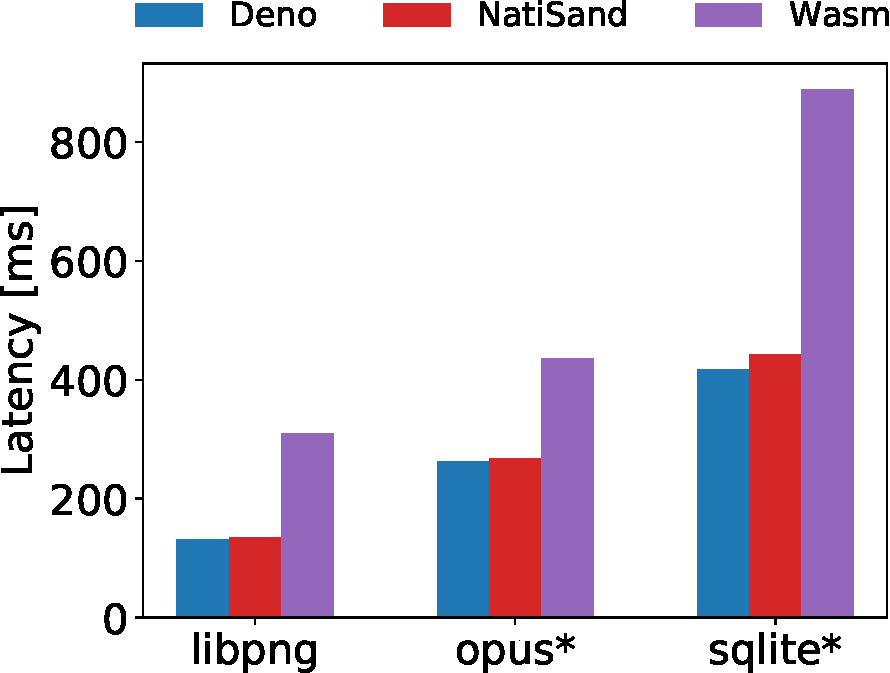
\includegraphics[width=\columnwidth]{chapters/natisand/fig/cropped-summary-ffi-latency.pdf}
	\end{subfigure}%
	\hspace{1em}
	\begin{subfigure}{0.47\columnwidth}
		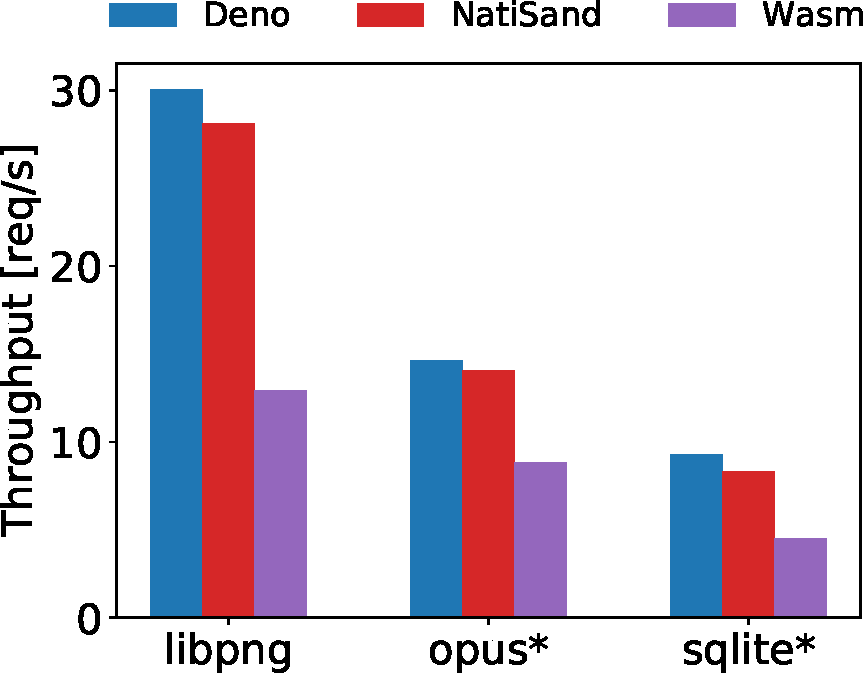
\includegraphics[width=\columnwidth]{chapters/natisand/fig/cropped-summary-ffi-throughput.pdf}
	\end{subfigure}
	\caption[Average latency and throughput of native-functions-based
		microservices]{
		Average latency and throughput for microservices that execute
		native functions (* marks the use of {\tt nativeCall})
	}
	\label{fig:native-lib-latecy-throughput}
\end{figure}

\paragraph{Usability}
%
While Wasm offers strong isolation guarantees, it also comes with drawbacks compared to \pap. First of all it requires the developer
to use a Wasm-compatible version of the library. In our evaluation we
used a precompiled version of sqlite3, but we had to manually compile
opus and libpng using the Emscripten toolchain~\cite{emscripten} and
the WASI Sdk~\cite{wasi-sdk}, respectively. Moreover, current implementations of the WebAssembly
System Interface (WASI) can only restrict ambient rights
programmatically, and filesystem privileges work at
directory granularity. Lastly, Wasm requires the developer to
explicitly allocate, write, and read bytes from the Wasm module linear
memory.


%%% Local Variables:
%%% mode: latex
%%% TeX-master: "../main.tex"
%%% End:

\section{Related work}
\label{natisand:rel_works}

Isolation of software has been widely investigated by both the academic
and industrial communities~\cite{berman1995tron, kim2013practical,
  demarinis2020sysfilter, minijail, sandbox2, firejail,
  bubblewrap,seapp,wasi-poster}.  {\em MBOX}~\cite{
  kim2013practical} features an unprivileged sandboxing mechanism that
prevents a process from modifying the host filesystem by layering the
sandbox filesystem on top of it. The solution is implemented by
interposing syscalls using Seccomp and {\em ptrace}. The use of {\em
  ptrace} required the authors careful attention to avoid the risk of
TOCTOU attacks, moreover it suffers from non-negligible performance
degradation. DeMarinis et al.~\cite{demarinis2020sysfilter} propose
{\em Sysfilter}, a static analysis framework to reduce the attack
surface of the kernel, by restricting with Seccomp the system call set
available to processes.  This approach proves to be effective in
limiting the kernel APIs that can be abused by attackers, but whenever
a system call is necessary for the benign behavior of a program, there
is no way to control with Seccomp the specific instance of the
resource used. {\em BPFBox}~\cite{ findlay2020bpfbox}, {\em
  BPFContain}~\cite{findlay2021bpfcontain}, and {\em
  Snappy}~\cite{belair2021snappy} are security frameworks that provide
confinement of processes and containers with the use of eBPF.  These
solutions highlight the benefit of eBPF by providing simple, efficient,
and flexible confinement of system resources, however these solutions
either require a privileged daemon or require to load kernel modules
to introduce a set of {\em dynamic helpers}.   Often,
industrial sandboxing solutions take advantage of multiple protection
techniques to support process containment. This is the case for {\em
  Minijail}~\cite{minijail}, and {\em Sandbox2}~\cite{ sandbox2}. Some
of the security mechanisms used are: introduction of new user ids,
capabilities restriction, namespace isolation and policy-based Seccomp
filtering. These tools expose a powerful interface meant
to be used by security experts. Similar considerations are shared with
other less mature tools such as {\em Firejail}~\cite{ firejail} and
{\em Bubblewrap}~\cite{bubblewrap}.

Multiple research efforts have studied the use of third-party
components in software products~\cite{RLBox, kirth2022pkru,
  wu2012codejail, cali}. {\em PKRU-Safe}~\cite{kirth2022pkru} proposes an
automated method for preventing the memory corruption of memory-safe
languages due to the interaction with unsafe code. It leverages the
compiler infrastructure to provide hardware-backed memory protection
requiring changes to build files, dependencies, and code (in the form
of code annotations). {\em Codejail}~\cite{wu2012codejail} provides
partial isolation of libraries by spawning a new process and
configuring the necessary communication channels to support tight
memory interactions with the main program. To support the change in
the interactions without modifications to the library code it is
necessary to write a wrapper library.
{\em Cali}~\cite{cali} is a compiler-assisted library
isolation system that compartmentalizes libraries into their own
process, and automates the configuration of the necessary
communication channels by tracking data flow between the program and
the library at link time.
{\em RLBox}~\cite{RLBox} is a
framework to isolate libraries in lightweight sandboxes -- i.e.,
process, Wasm. It facilitates the retrofitting of applications
employing static information flow enforcement and dynamic checks
expressed in the C++ type system. These solutions were designed for
compiled languages, so while some of the concepts are portable to JS
runtimes, the solutions are not easily adapted to this domain.

A recent study by Staicu et al.~\cite{staicu2021bilingual} highlights
how the possibility to invoke native code from scripting languages
undermines the security assumption of applications. They discuss a
methodology to detect misuses of the native extension API and show how
the exploit of these vulnerabilities in npm packages can lead to web
applications compromise. Previous proposals~\cite{
  vasilakis2018breakapp, wyss2022wolf, binwrap} tackle this problem by
providing solutions to isolate the execution of third-party
modules. {\em Wolf at the Door}~\cite{wyss2022wolf} reduces the risk
associated with the installation of npm packages by mediating their
install-time capabilities. It enforces complex user-defined policies
by leveraging AppArmor, hence prohibiting unauthorized access to
confidential files and connections using an LSM that currently cannot
coexist with SELinux and SMACK. {\em BreakApp}~\cite{
  vasilakis2018breakapp} takes advantage of module boundaries to
compartmentalize npm modules in accordance with a set of code
annotations. Modules are isolated with software, process, or container
isolation, and it is possible to configure the visibility of the
application context available to external modules. Process and
container isolation enable the protection of native code, however the
specification of their permissions are beyond the scope of the
proposal.
{\em Cage4deno}~\cite{cage4deno} protects filesystem resources from subprocesses
executed by JavaScript runtimes.
{\em BinWrap}~\cite{binwrap} separates the execution of
third-party components from the rest of the application using distinct
execution threads for different domains of trust. The main focus
of the proposal is prohibiting arbitrary accesses to sensitive data
stored in the memory of the JS runtime by leveraging Intel's MPK/PKU.
\pap is complementary to the above solutions since our goal
is to specify and enforce permissions on native code dependencies of
web applications, rather than providing memory isolation for
untrusted components.

Protecting JS code from being compromised is out of the scope of \pap,
nonetheless, since proposals in this domain and ours both target the
web development audience, our proposal shares some ideas with previous
works in this domain~\cite{vasilakis2021preventing, sandtrap,
  terrace2012javascript, ntousakis2021detecting}. For instance, Ferreira et al.~\cite{
  npm-malicious-update} propose a lightweight permission system providing
per-package on/off switches that limit access to Node.js core modules
(e.g., child\_process, fs, http). By doing so, it can prohibit access
to subprocess, filesystem, and network resources for the JS
code. Similarly, \pap takes care of protecting filesystem, IPC, and
network resources, targeting native code. {\em Mir}~\cite{
  vasilakis2021preventing} is a system preventing the compromise of
the application by third-party modules with the enforcement of
fine-grained RWX permissions on every field of every variable in the
JS context. \pap adopts an equivalent permission model to contain
native code when accessing filesystem resources. Another research work
enforcing security boundaries stated in a policy is {\em
  SandTrap}~\cite{sandtrap}. The approach enforces fine-grained
access control policies on cross-domain interactions between
application code and the third-party modules. The creation of policy
files described by the authors consists in running test suites to
create a policy with acceptable static cross-domain interaction
coverage. We adopt a similar approach in the policy generation of
\pap. Note that, differently from our proposal, solutions protecting
JS code can run in user space, thus they do not limit the portability
of the JS runtime to Linux systems.

%%% Local Variables:
%%% mode: latex
%%% TeX-master: "../main.tex"
%%% End:

\section{Conclusions}

The increase in scale and complexity of modern web applications has
led to the introduction of new security mechanisms in JS
runtimes. Unfortunately, native code execution still represents
a clear risk, since no isolation is provided by all the major
platforms. \pap solves this problem, introducing new measures to
confine the execution of binaries and shared libraries. The
proposal is not dependent on a particular JS runtime, and was designed
to be integrated into different architectures.  Considerable
attention was dedicated to usability; little effort is required by
developers to sandbox their applications. Indeed, no specific security
expertise is necessary to benefit from the protection, nor
are changes to the application.

We believe that the approach proposed in this chapter can contribute to
improve the state of the art in this domain and support the evolution
toward more secure software platforms.

%%% Local Variables:
%%% mode: latex
%%% TeX-master: "../main.tex"
%%% End:


\section*{Availability}
The source code and the artifacts produced to support the proposal are
available open source at \url{https://github.com/unibg-seclab/natisand}

% \begin{acks}
% The work was supported by the European Commission within the GLACIATION
% project (No 101070141) and by project GRINS (PE00000018) under the MUR
% NRRP funded by the EU - NextGenerationEU.
% \end{acks}


\chapter[Conclusions and future work]{Conclusions and future work}
\label{chap:conclusions}
In this thesis, we presented novel fine-grained access control
techniques to protect resources in mobile and cloud applications.

We opened our dissertation by describing \seapp, a technique for
mitigating security threats in the Android mobile operating system.
\seapp empowers developers with the capability of isolating the
internal components of Android apps and regulate their permissions on
a per-component basis. This crucial step not only limits the impact a
vulnerability has on the app resources, but it also allows to provide
strong user privacy guarantees and meet data privacy regulations
despite the use of third-party code.

The dissertation proceeded considering the importance to also secure
cloud applications. Specifically, we presented an approach to support
the introduction of security policies to restrict the file system
resources available to an application. Compared to virtualization
technologies such as VMs and containers, which are associated with
coarse granularity, we demonstrate that our proposal enables the
introduction of fine-grained, per-resource access rules. Then, we
further explore the topic in the context of WebAssembly runtimes.
Here, not only the approach permits to introduce fine-grained
policies to restrict file system access, it also replaces error-prone
userspace implementations of the security checks (and the security
issues stemming from them) with a unified eBPF implementation.
Finally, we consider the specific use of JavaScript runtimes for the
creation of cloud applications, and how developers commonly rely on
native code to speed up development and execution of the application.
Since JS runtimes do not provide solutions for the isolation of native
code, we propose \natisand, a runtime-agnostic component to control
the filesystem, Inter-Process Communication (IPC), and network
resources available to binary programs and shared libraries.

During our research work, considerable attention was dedicated to the
performance and usability of our proposals. The work presented in this
thesis represent the final result of multiple improving iterations to
ensure small performance footprint and high usability by developers.
Indeed, these are very important aspects since the lower the
performance side-effects and the effort on behalf of the developer to
integrate our solutions with existing applications, the broader will
be the adoption of our security mechanisms. With this regard, to
facilitate the integration of our solutions with existing real systems
and foster the reproducibility of our experimental evaluations, our
prototype implementations are all available open source.

We believe the approaches proposed in this thesis contribute to
improving the state of the art in this domain and support the
evolution toward more secure mobile and cloud software platforms.

\section{Future work}

This section concludes the thesis with a discussion on the future work
that can be done in the area of fine-grained access control
technologies to protect resources in mobile and cloud applications.

\noindent{\bf Mobile applications} -- Chapter~\ref{chap:seapp}
describes \seapp, a novel proposal that provides developers with a
mechanism to isolate the internal components of Android apps and
regulate their permissions on a per-component basis. This is
achieved by first executing components in dedicated processes, and
then restricting access to the app and system resources with ad hoc
\sel policies. While effective, the decision to use \sel to constraint
the access of application components impose significant limitations.
Resource-wise, \sel implies the use of process isolation to isolate
different components of the application; this increases CPU and memory
utilization which negatively affect responsiveness and battery life of
the mobile device. Usability-wise, despite our efforts, \sel policies
are hard to audit, author and maintain. Therefore, we consider the
possibility of replacing \sel and process isolation with novel Linux
Security Modules and memory protection techniques an interesting and
promising evolution of our work with the potential to solve both these
limitations and, thus, further promote adoption.

\noindent{\bf Cloud applications} -- Chapter~\ref{chap:dmng},
~\ref{chap:wasm}, and~\ref{chap:natisand} highlight limitations of the
cloud technologies available at the time of writing with regard to
fine-grained access control of system resources. Each chapter provides
its own take on a specific aspect of the problem.
Chapter~\ref{chap:dmng} relies on instrumentation to collect and audit
the activity traces generated by microservices, and then uses this
information to create fine-grained access control policies and
strengthen the security boundary of the cloud application.
Chapter~\ref{chap:wasm} focuses on the security implications of
enabling access to system resources through the WebAssembly System
Interface (WASI), and proposes improvements in the controlling access
to file system resources. Chapter~\ref{chap:natisand} considers the
use of JS runtimes for the implementation of cloud applications, and
proposes \natisand, a component to control the filesystem,
Inter-Process Communication (IPC), and network resources available to
binary programs and shared libraries. Interesting future work could
extend the observability and protection to a wider set of system
resources. For example, the use of memory protection techniques could
restrict the area affected by an attack to the sole exploited thread
without leading to potential compromise of the entire JS runtime.
Finally, given the flexibility and versatility of our designs another
interesting future work would be the adoption of these techniques to
secure other Wasm and JS runtimes, or even other interpreted languages
(e.g., PHP, Python, and Ruby).


% -------------------- APPENDIX ------------------- %

\appendix

% seapp appendix
\chapter[Seapp documentation]{SEApp documentation}\label{appendix:seapp_analysis}

\vspace{-1.8em}
\begin{wrapfigure}{r}{0.3\textwidth}
  \vspace{-1.5em}
	\begin{center}
          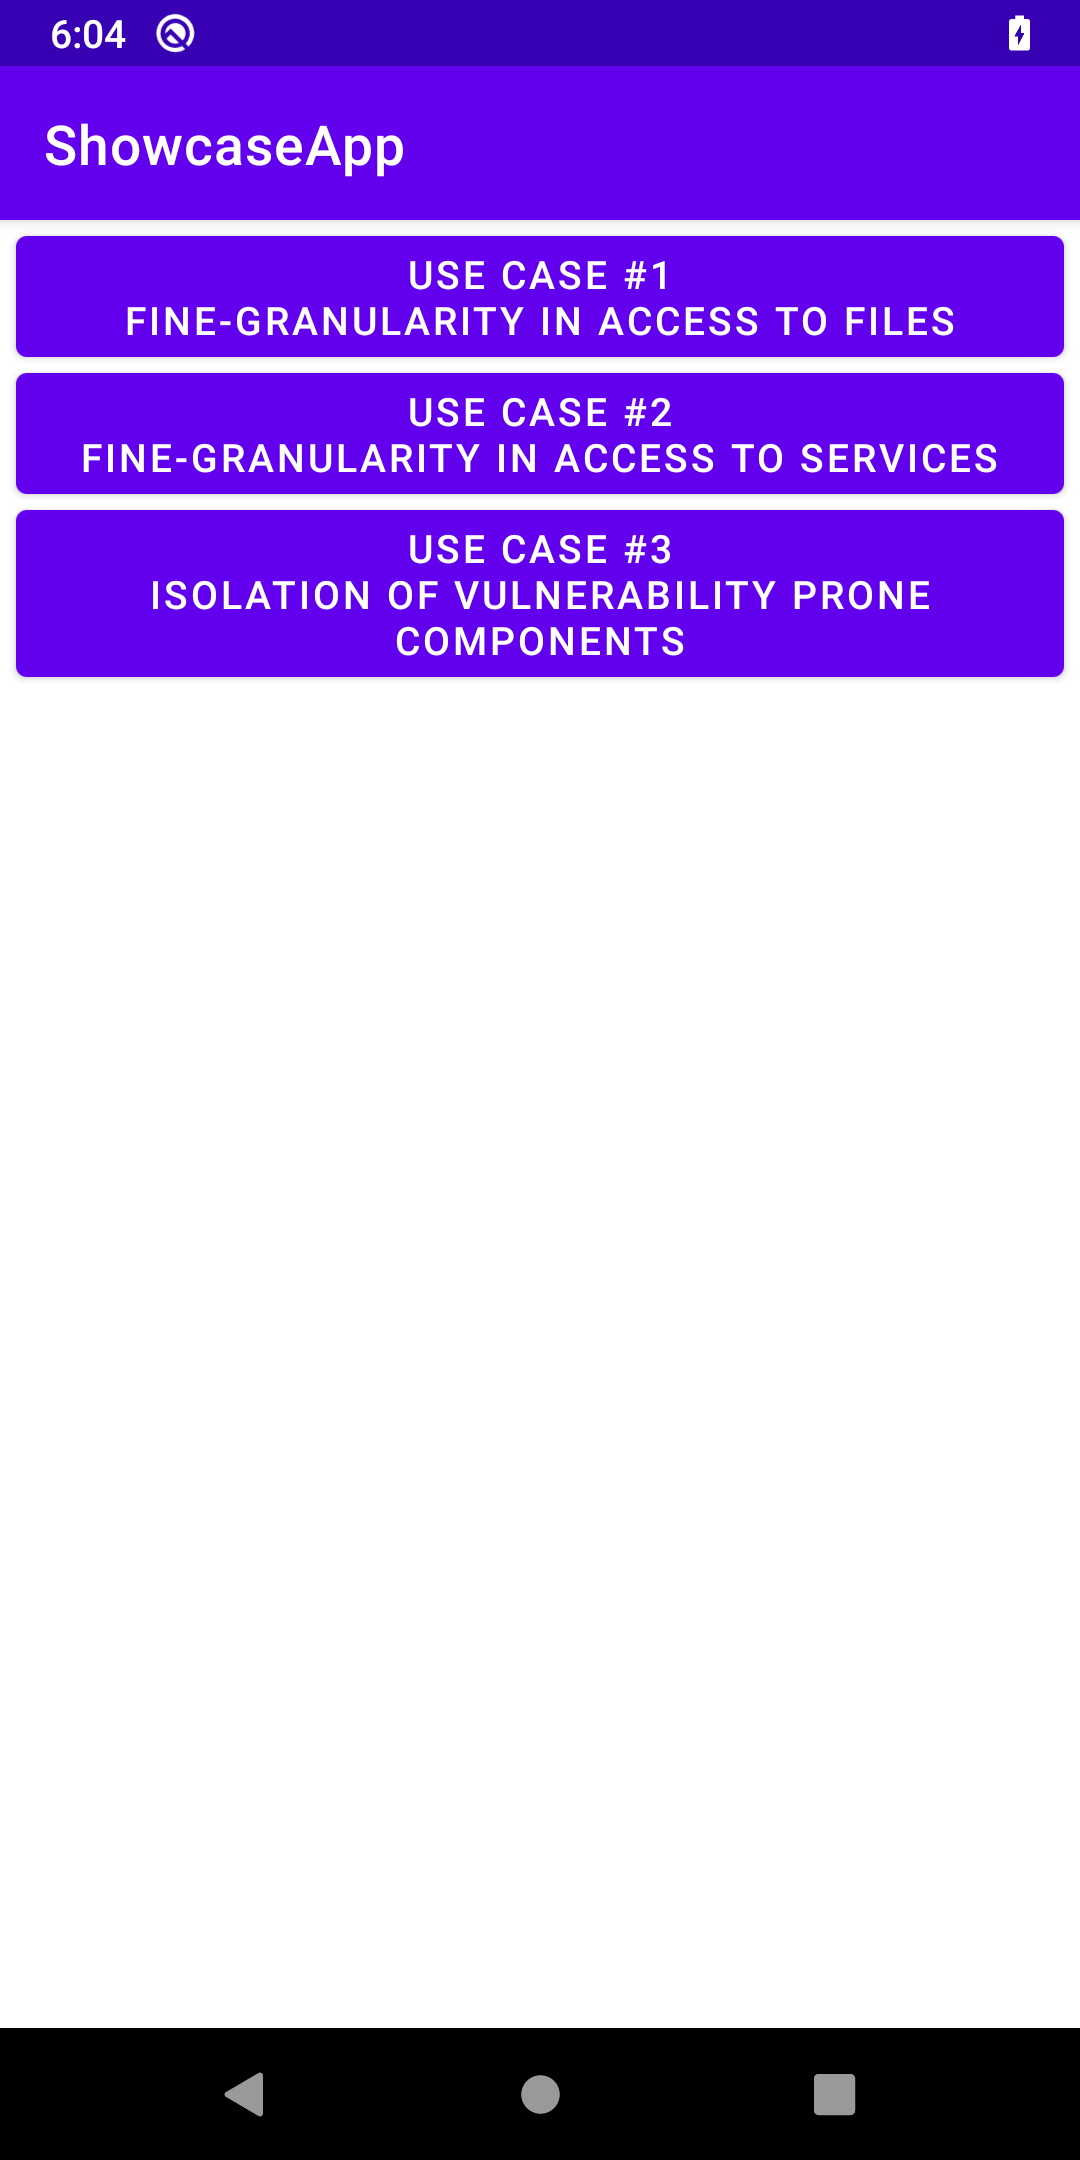
\includegraphics[width=0.28\textwidth]{chapters/seapp/figs/ae/MainActivity.png}
        \end{center}
	\caption{ \bf MainActivity}
	\label{fig:seapp_mainactivity_view}
      \end{wrapfigure}
      
\vspace{-1em}
This chapter gives a technical demonstration of the security measures
introduced by \pap. The description is based on the showcase app
presented in Section~\ref{sect:seapp_motiv}. We show that: (1) the
showcase app can operate without a policy module; in this mode, its
vulnerabilities can be exploited; (2) the showcase app can also
operate with the policy module listed in
Appendix~\ref{appendix:seapp_policy} and use the services offered by
SEApp; in this mode, the internal vulnerabilities are no longer
exploitable.

The showcase app has a minimal structure. Its entry point is the {\em
  MainActivity} (Figure~\ref{fig:seapp_mainactivity_view}), which is associated with the {\em core\_logic}
process. From the {\em MainActivity} it is possible to send a {\em
  startActivity} intent to one among {\em UseCase1Activity}, {\em
  UseCase2Activity} and {\em UseCase3Activity}; the entry points of
use cases~1, 2 and~3, respectively. For each entry point {\em Zygote}
starts a dedicated process and, according to the content of the
\seappcontexts (in Listing~\ref{seapp_seappctxp}), assigns its
specific domain ({\tt user\_logic\_d} to UC\#1, {\tt ads\_d} to UC\#2,
{\tt media\_d} to UC\#3).  A dedicated description of each use case
follows.

\vspace{-1.6em}\section{Use case 1}\label{appendix:seapp_uc1}

\vspace*{-0.5em}
In this use case we demonstrate how an app could benefit from the
fine-granularity access to files.  In particular, we show how the {\em
  UseCase1Activity}, suffering of a path traversal vulnerability,
cannot be exploited when the app is associated with a properly
configured policy module.  According to the Google Play Protect report
on common application
vulnerabilities~\cite{seapp_common_play_protect_vulnerabilites},
unsanitized path names that lead to path traversal are a primary
source of problems in applications.

{\em UseCase1Activity} is quite simple: it displays the content of a
file given its relative path through an intent
(Figure~\ref{fig:seapp_uc1_views}a). While this may be fine when the
intent comes from trusted components, the activity supports also
implicit intents coming from untrusted sources. This makes the
vulnerability easily exploitable by an attacker targeting the
confidential files written by the {\em core\_logic} components.
%
In our setup phase, we leverage {\em MainActivity} to create an
internal directory structure by using the {\tt android.os.File}
abstraction, which sets file and directory context upon its creation
(see Section~\ref{sect:seapp_impl_files}). Two directories are
created: {\tt user/} and {\tt confidential/}; inside both folders a
file {\tt data} is saved.
%
To test this use case, we first start {\em UseCase1Activity}, then we
send an intent to ``confuse'' {\em UseCase1Activity} into showing us
the content of {\tt confidential/data}. This can be done via ADB with
the command:
\begin{lstlisting}[numbers=none]
adb shell am start
-n com.example.showcaseapp/.UseCase1Activity
-a "com.example.showcaseapp.intent.action.SHOW"
--es "com.example.showcaseapp.intent.extra.PATH" "../confidential/data"
\end{lstlisting}
\normalsize

When the policy module is not availableg, all app internal files are
flagged with {\tt app\_data\_file} and every app component executes
within the {\tt untrusted\_app} domain, which holds read access to
{\tt app\_data\_file}. As a consequence the vulnerability is
successfully exploited and {\em UseCase1Activity} shows the content of
the {\tt confidential/data} file (Figure~\ref{fig:seapp_uc1_views}b).

Instead, when the policy module is available, the file {\tt
  confidential/data} is flagged with {\tt confidential\_t}, as
indicated in line 2 in \filecontexts (see
Listing~\ref{seapp_filectxp}). Since no permission is granted on {\tt
  confidential\_t} in the \sepolicy to {\tt user\_logic\_d}, any
access to the file {\tt confidential/data} by {\em UseCase1Activity}
is blocked by \sel (Figure~\ref{fig:seapp_uc1_views}c). The following
denial is written to the system log: {\em denied {\tt search} to {\tt
    user\_logic\_d} domain on {\tt confidential\_t} type}
(Figure~\ref{fig:seapp_uc1_logcat}). The {\tt confidential} directory
cannot then be accessed despite the exploitation of the path traversal
vulnerability.

\begin{figure}[h!]
  \centering
  \subfloat{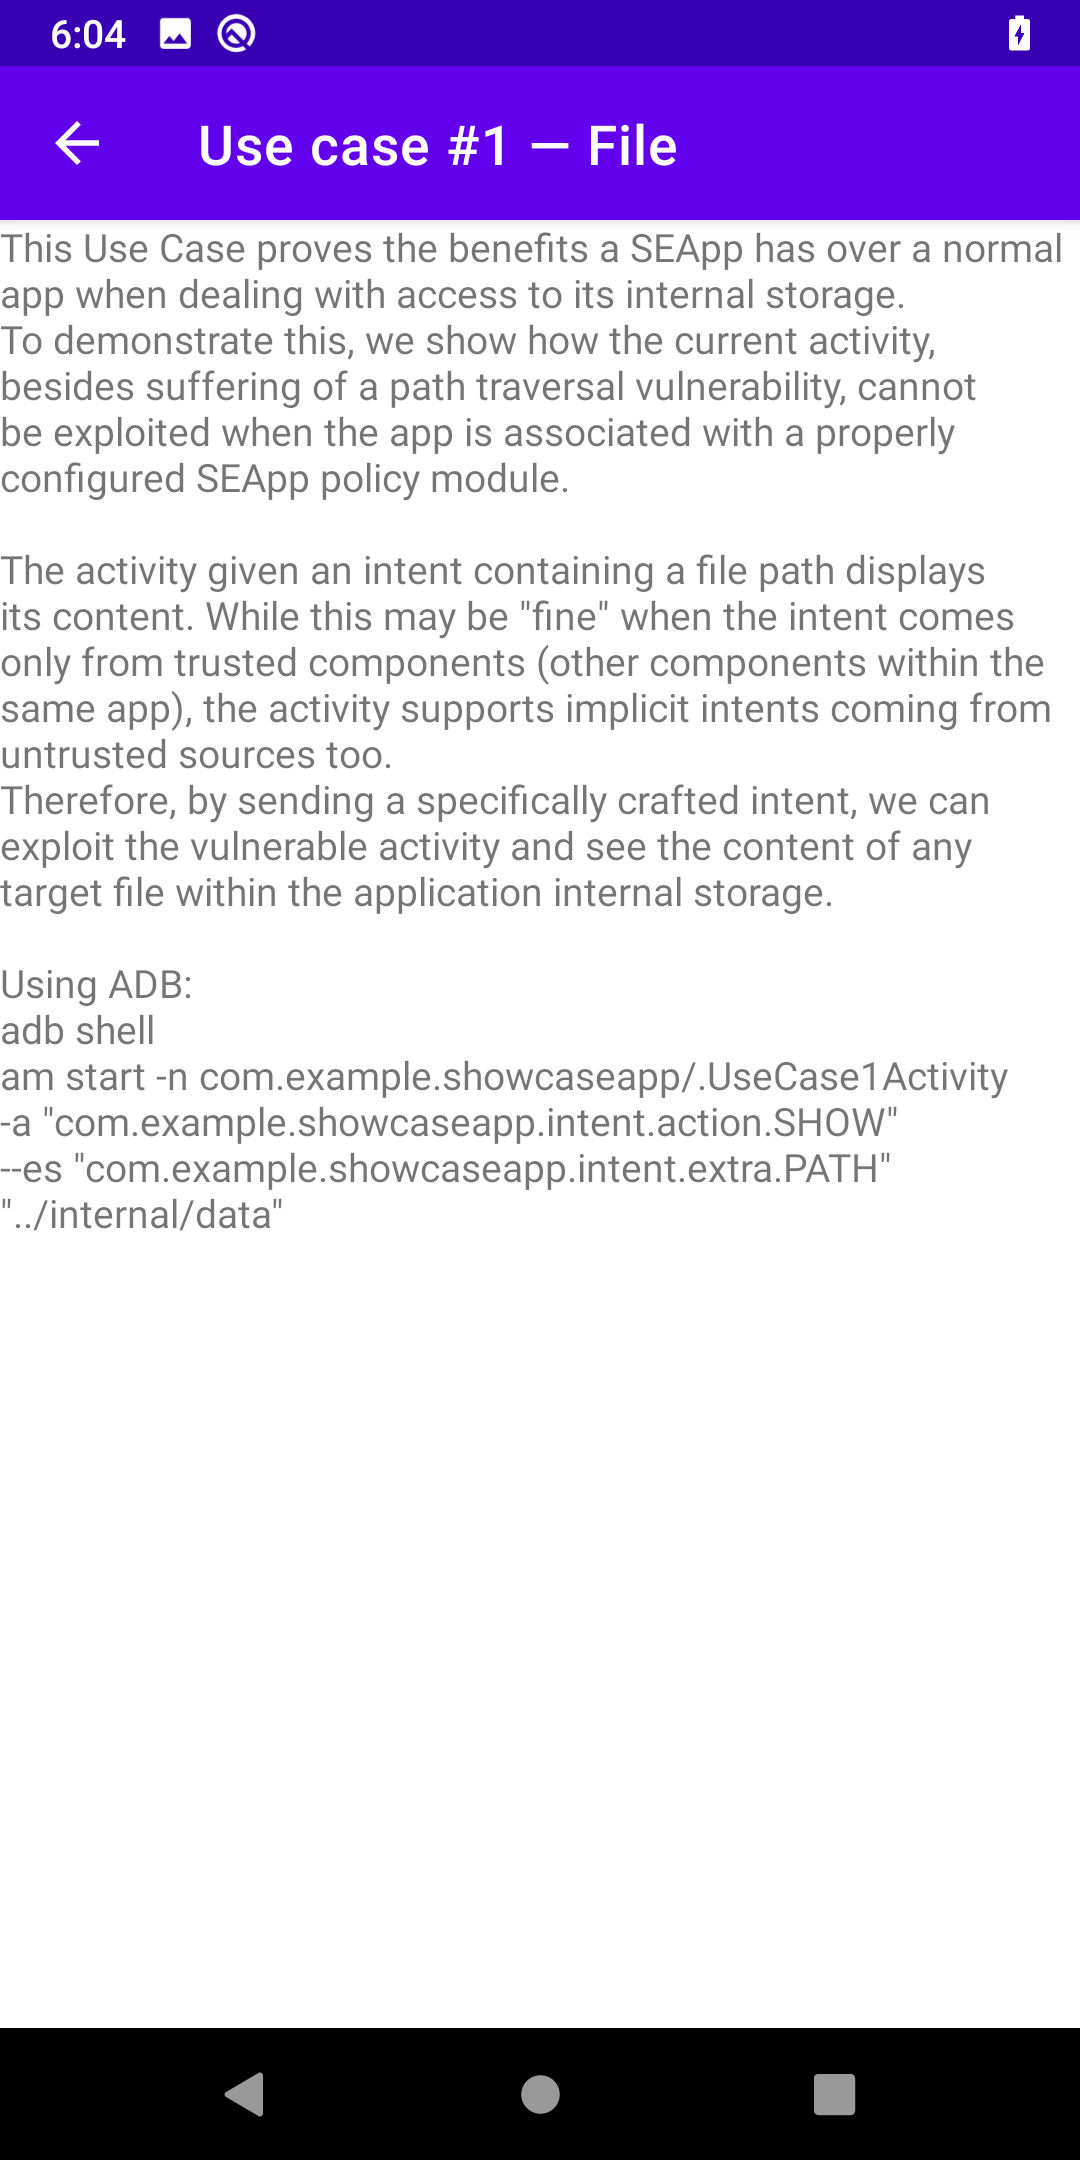
\includegraphics[width=0.28\textwidth]{chapters/seapp/figs/ae/UseCase1Activity.png}}
  \hfill
  \subfloat{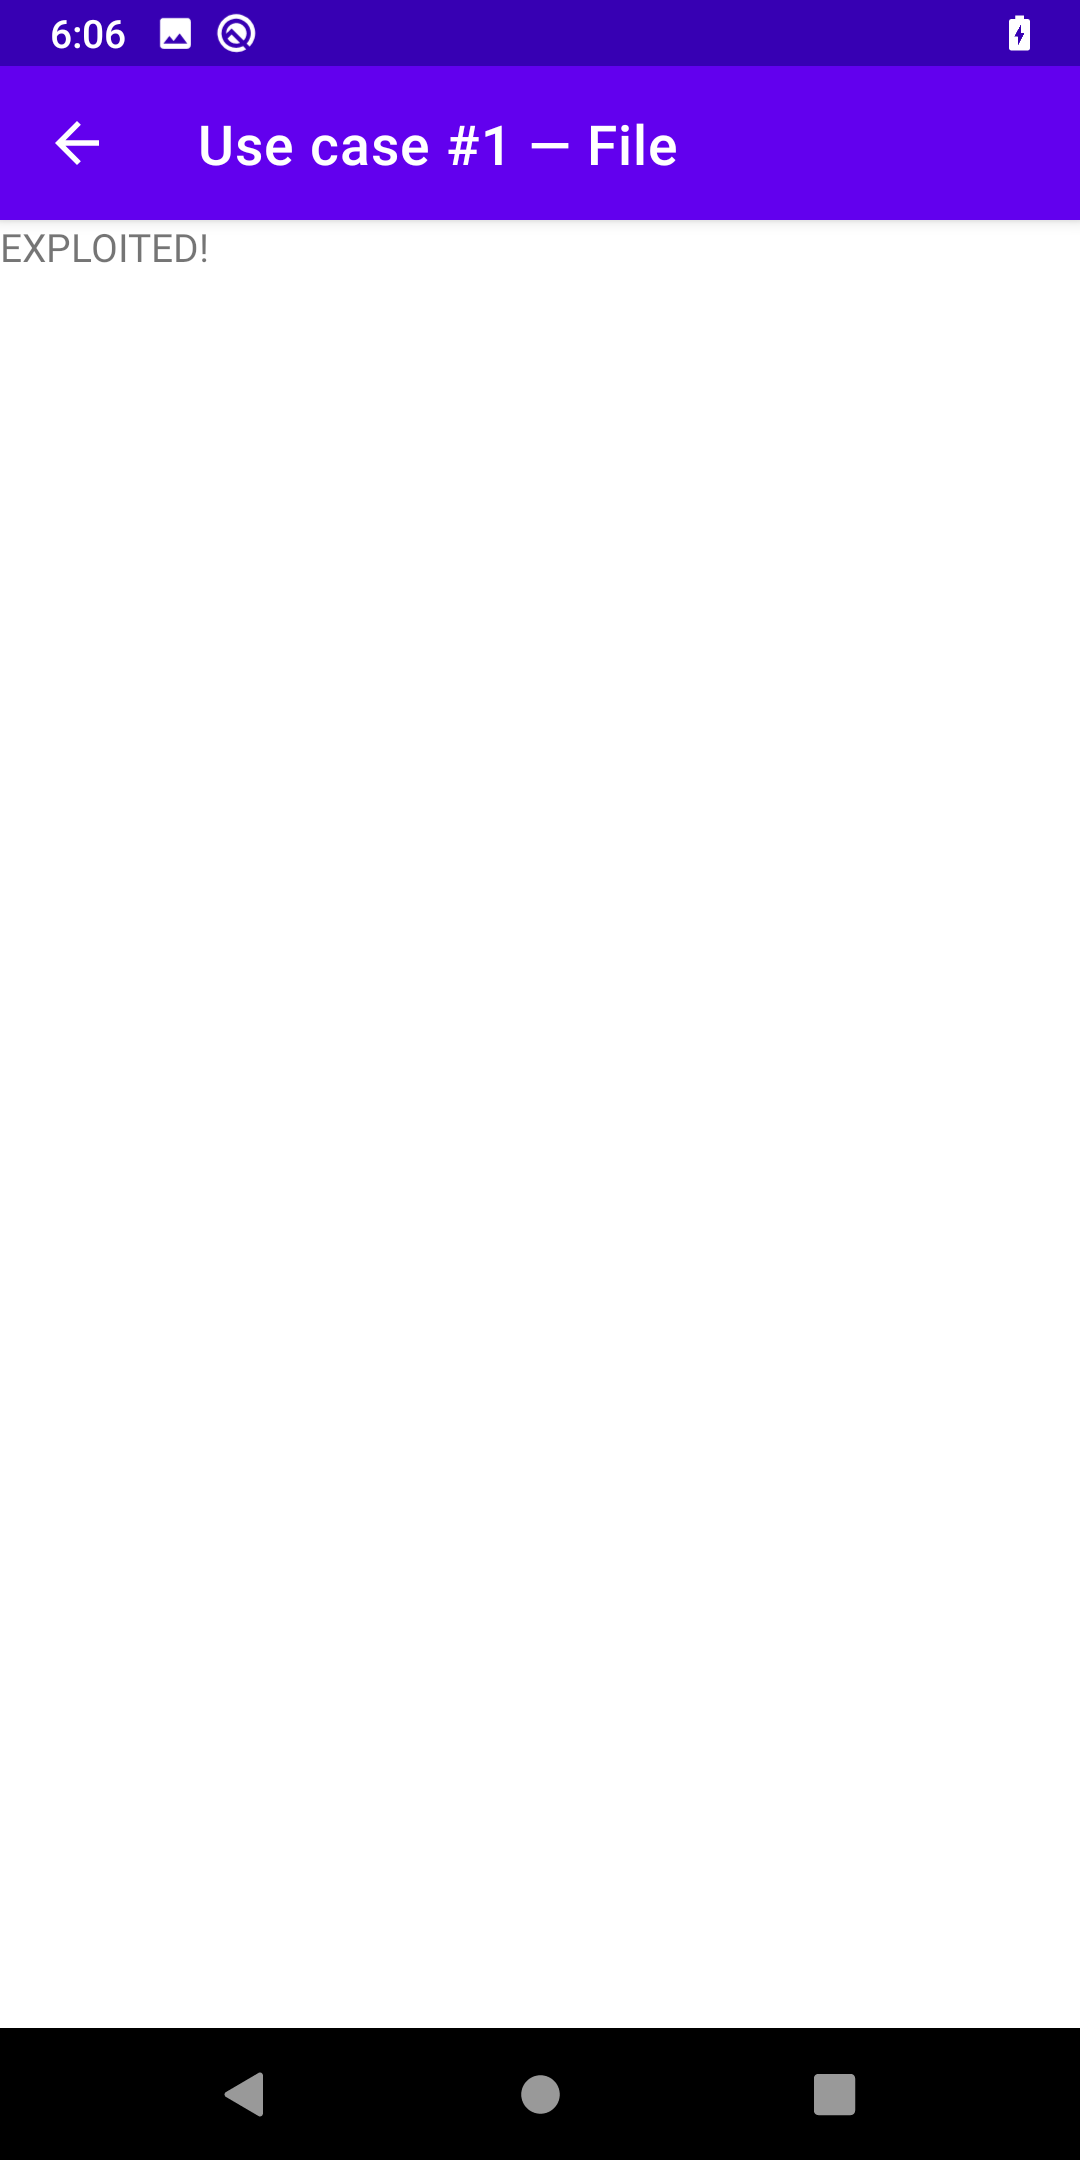
\includegraphics[width=0.28\textwidth]{chapters/seapp/figs/ae/UsaCase1ActivityExploited.png}}
  \hfill
  \subfloat{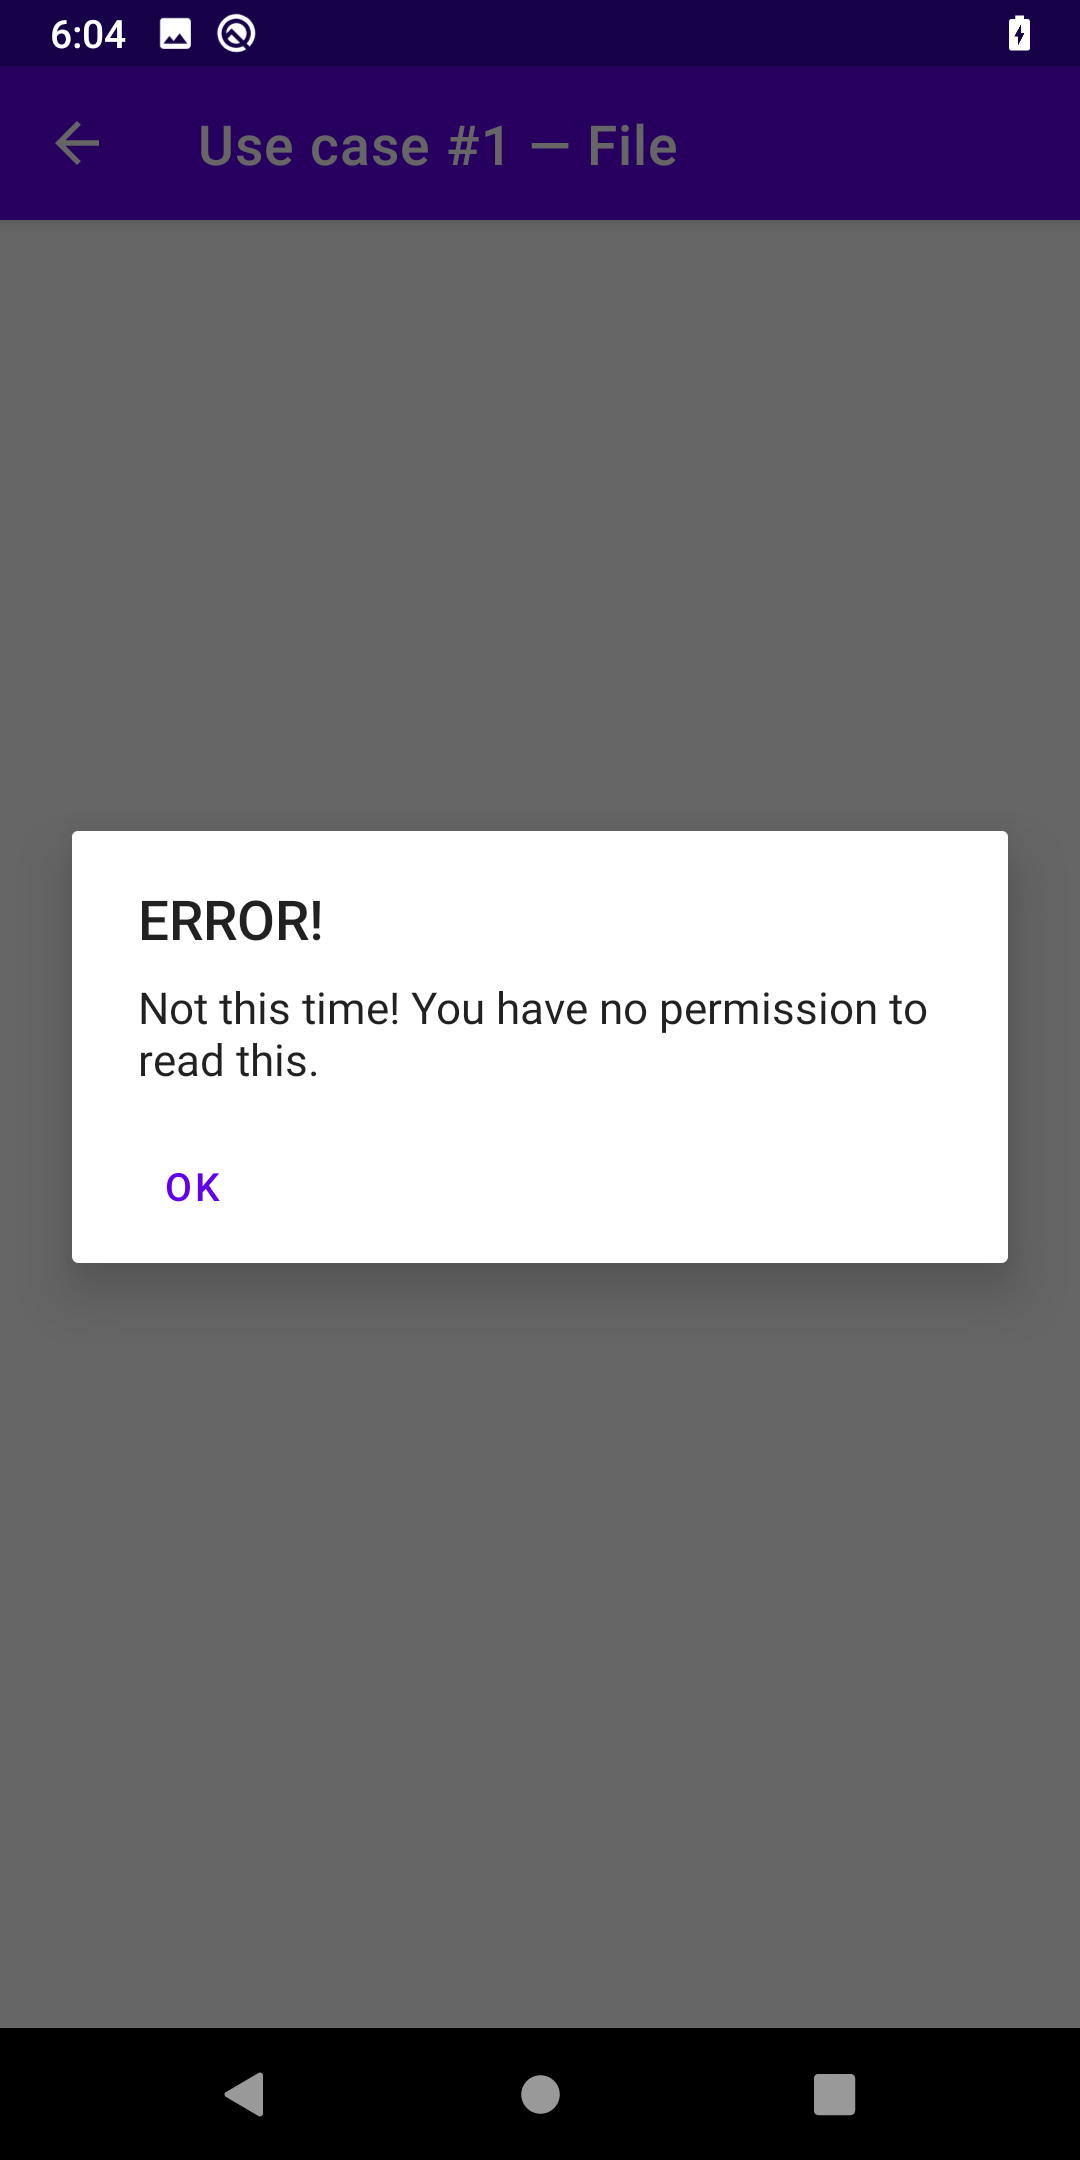
\includegraphics[width=0.28\textwidth]{chapters/seapp/figs/ae/UseCase1ActivityNotExploited.png}}
  \caption{\label{fig:seapp_uc1_views}\bf Use case 1 views}
\end{figure}

\begin{figure}[h!]
  \centering
  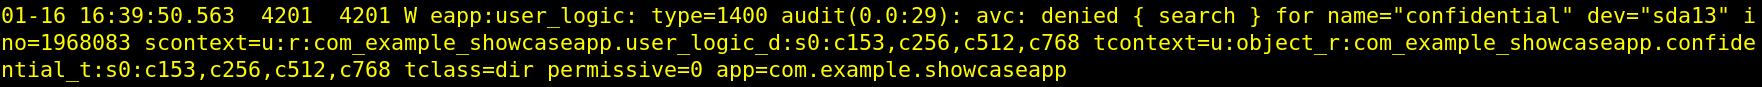
\includegraphics[width=\textwidth]{chapters/seapp/figs/ae/UseCase1Logcat.png}
  \caption{\label{fig:seapp_uc1_logcat}\bf Use case 1 logcat}  
\end{figure}

\newpage
      

%%% Local Variables: 
%%% mode: latex
%%% TeX-master: "../../../../main.tex"
%%% reftex-default-bibliography: "../../../../bib/biblio.bib"
%%% End:

\section{UC\#2: fine-granularity in access to services}\label{appendix:seapp_uc2}

In this use case we show how to confine an Ad library into an ad-hoc
process, with guarantees that it cannot abuse the access privileges
granted to the whole application sandbox by the user.  To do that, we
deliberately inject, in the same process the library is executed, a
malicious component (which is directly invoked by the library) that
tries to capture the location when the permission {\em
  ACCESS\textunderscore FINE\textunderscore LOCATION} is granted to
the app. The Ad library used is Unity Ads~\cite{seapp_unityads}, which
according to~\cite{seapp_ads_use} in 2020 was used by 11\% of apps
that show ads.
%
\begin{figure}[h]
  \centering
  \subfloat{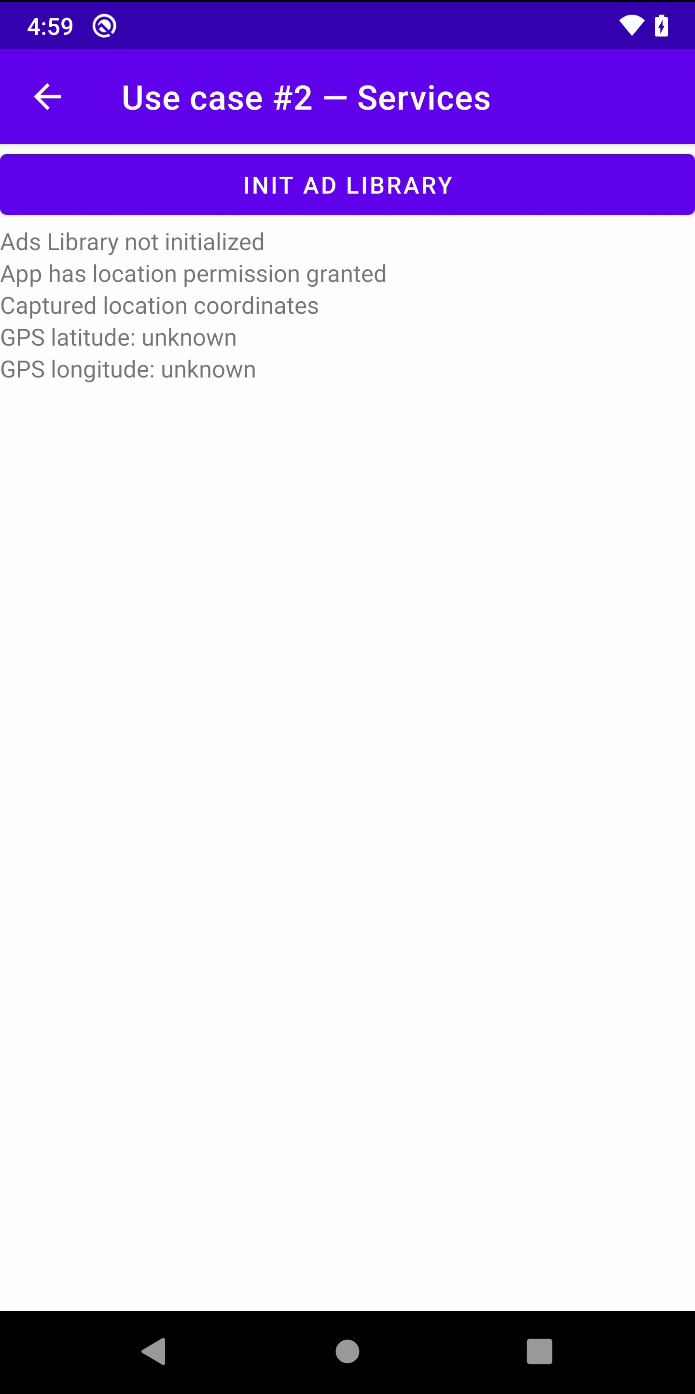
\includegraphics[width=0.3\textwidth]{chapters/seapp/figs/ae/uc21.png}}
  \hfill
  \subfloat{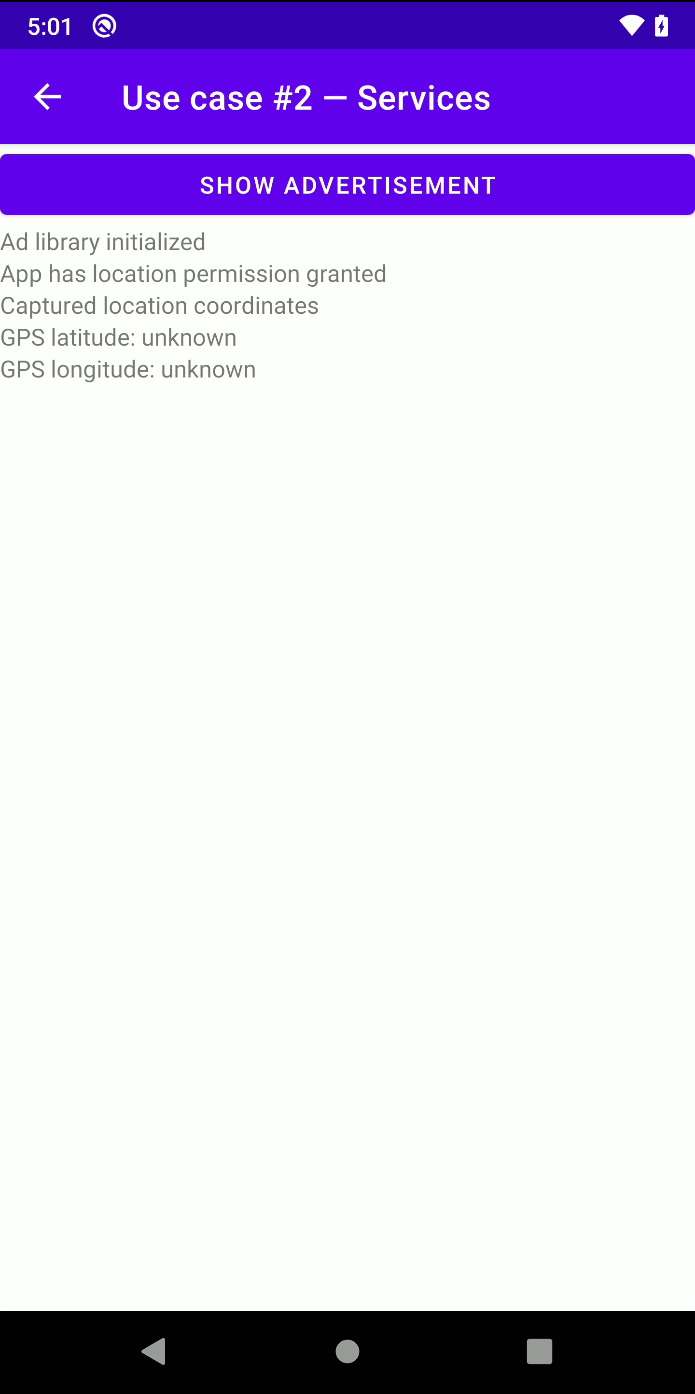
\includegraphics[width=0.3\textwidth]{chapters/seapp/figs/ae/uc22.png}}
  \hfill
  \subfloat{
\includegraphics[width=0.3\textwidth]{chapters/seapp/figs/ae/uc23.png}}
  \caption{\label{fig:seapp_uc2_views} UC\#2 views}
\end{figure}

In this case the library is invoked by {\em UseCase2Activity}
(Figure~\ref{fig:seapp_uc2_views}a), and according to line 3 of the
\seappcontexts, both the activity and the components created by the
library are executed by {\em Zygote} in a process labeled with {\tt
  ads\_d}.  To interact with the Ad library, {\em UseCase2Activity}
instances a {\tt UnityAdsListener}.  After the Ad initialization
(including the registration of the listener) and displaying the Ad to
the user (Figures~\ref{fig:seapp_uc2_views}b-c), the Ad framework
invokes the listener callback method {\tt onUnityAdsFinish}, which
executes the malicious routine {\tt captureLocation}. The routine
probes the app permissions; if {\em ACCESS\textunderscore
  FINE\textunderscore LOCATION} is granted to the app, the malicious
component retrieves through the \servicemanager a handle to the {\tt
  LocationManager}, and registers to it an asynchronous listener to
capture GPS location (Figure~\ref{fig:seapp_uc2_exploit}).

We show that when the policy module is enforced by \seapp, the malicious
component cannot access the GPS coordinates. This is because the
component is executed in the same process of the library, which is
labeled with {\tt ads\textunderscore d}. If we look at the \sepolicy
(lines 43-50), {\tt ads\_d} is not granted access to the \sel type
{\tt location\textunderscore service}, so the malicious routine cannot
retrieve and therefore connect to the {\em location\textunderscore
  service}.  The following denial is written to the system log: {\em
  denied {\tt find} on {\tt location\textunderscore service} to the
  {\tt ads\textunderscore d} domain}
(Figure~\ref{fig:seapp_uc2_logcat1}). As a result, the malicious
component is terminated by the {\em ActivityTaskManager}
(Figure~\ref{fig:seapp_uc2_logcat2}).

The Ad library was included in the app as an {\em .aar}
archive. To confine it, no modification was necessary, only
the use of \manifest and \sepolicy was required.

\begin{figure}[h]
  \centering
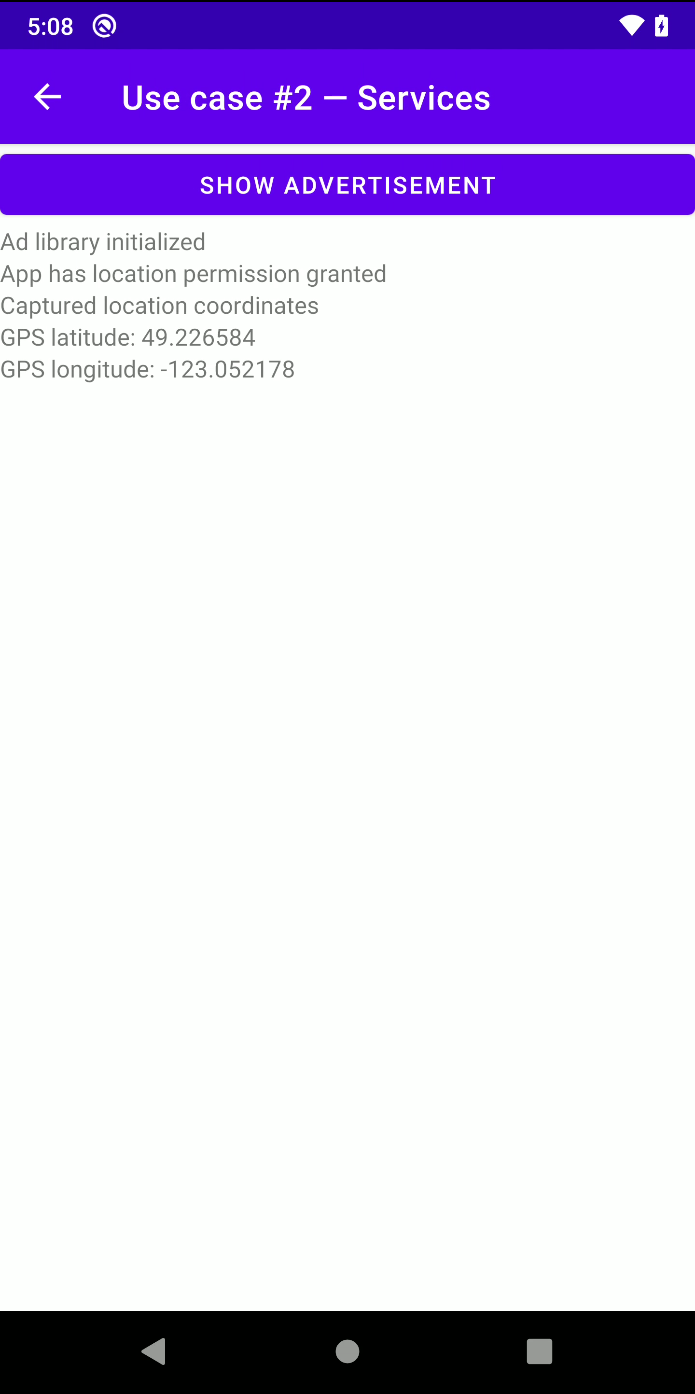
\includegraphics[width=0.29\textwidth]{chapters/seapp/figs/ae/uc24.png}
  \caption{\label{fig:seapp_uc2_exploit} UC\#2 malicious gadjet retrieves location data}
\end{figure}  

\begin{figure}[h]
  \centering
  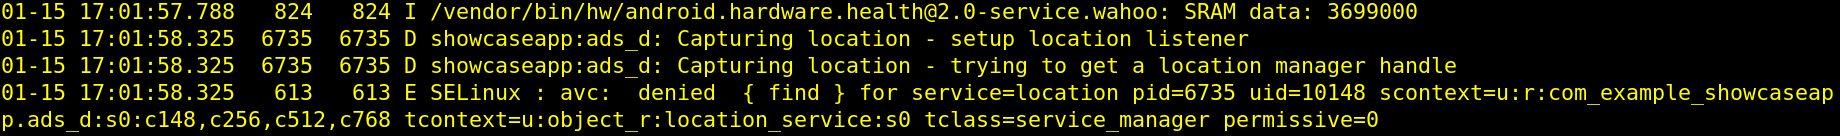
\includegraphics[width=\textwidth]{chapters/seapp/figs/ae/uc25.png}
  \caption{\label{fig:seapp_uc2_logcat1} UC\#2 \sel denial message in the system log}
\end{figure}      

\begin{figure}[h]
  \centering
  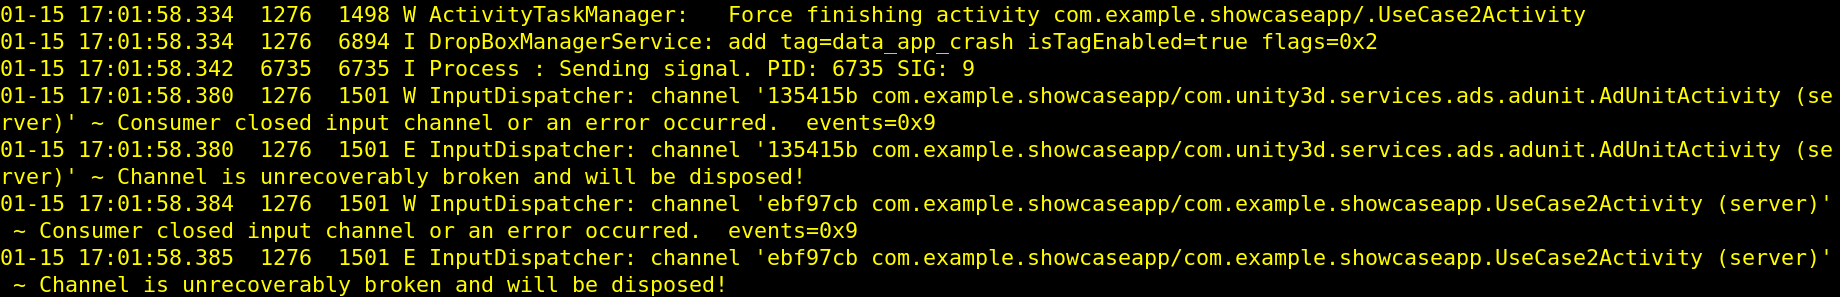
\includegraphics[width=\textwidth]{chapters/seapp/figs/ae/uc26.png}
  \caption{\label{fig:seapp_uc2_logcat2} UC\#2 activity termination due to \sel denial}
\end{figure}      


%%% Local Variables: 
%%% mode: latex
%%% TeX-master: "../../../../main.tex"
%%% reftex-default-bibliography: "../../../../bib/biblio.bib"
%%% End:

\newpage
\section{Use case 3}\label{appendix:seapp_uc3}

In this use case we show how to confine a set of components, which
rely on a high performance native library written in C to perform some
task. Our goal is to demonstrate that the context running the native
library code is prevented to access the network, even when the
permissions {\em INTERNET} and {\em ACCESS\textunderscore
  NETWORK\textunderscore STATE} are granted to the app sandbox.

\begin{figure}[h]
  \centering
  \subfloat{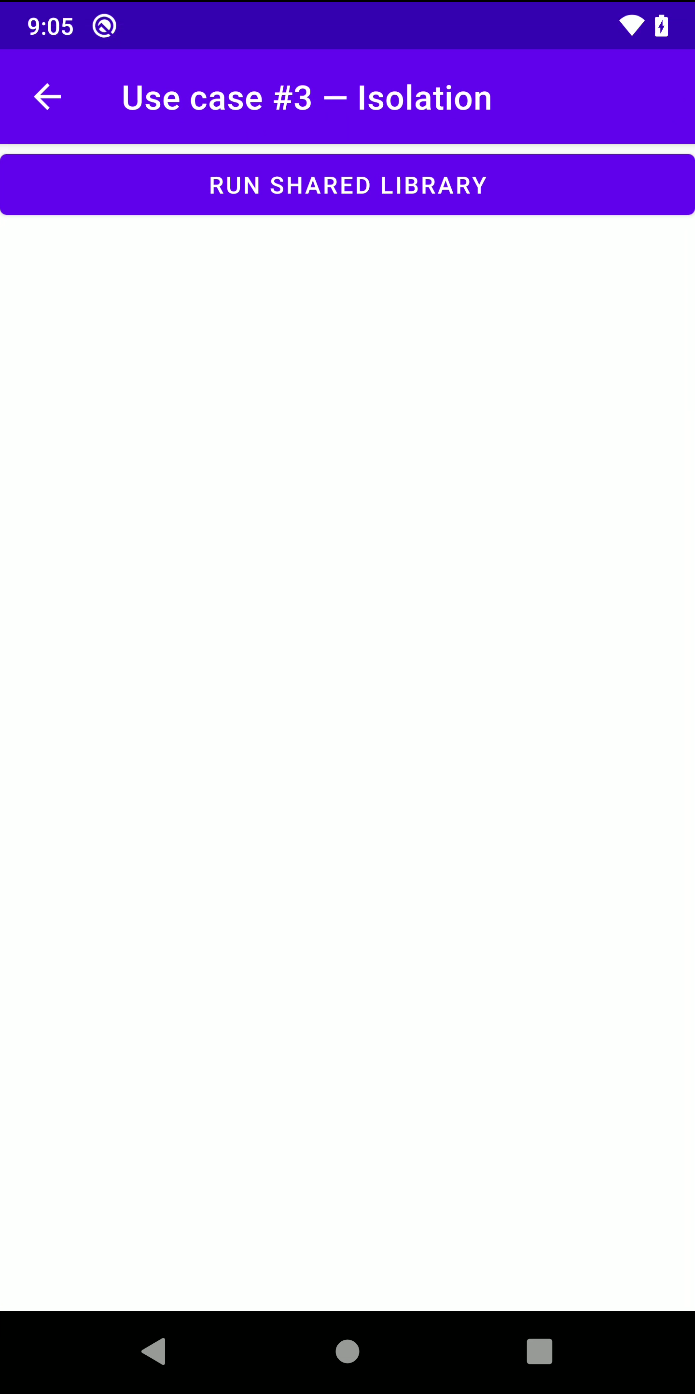
\includegraphics[width=0.3\textwidth]{chapters/seapp/figs/ae/uc31.png}}
  \hfill
  \subfloat{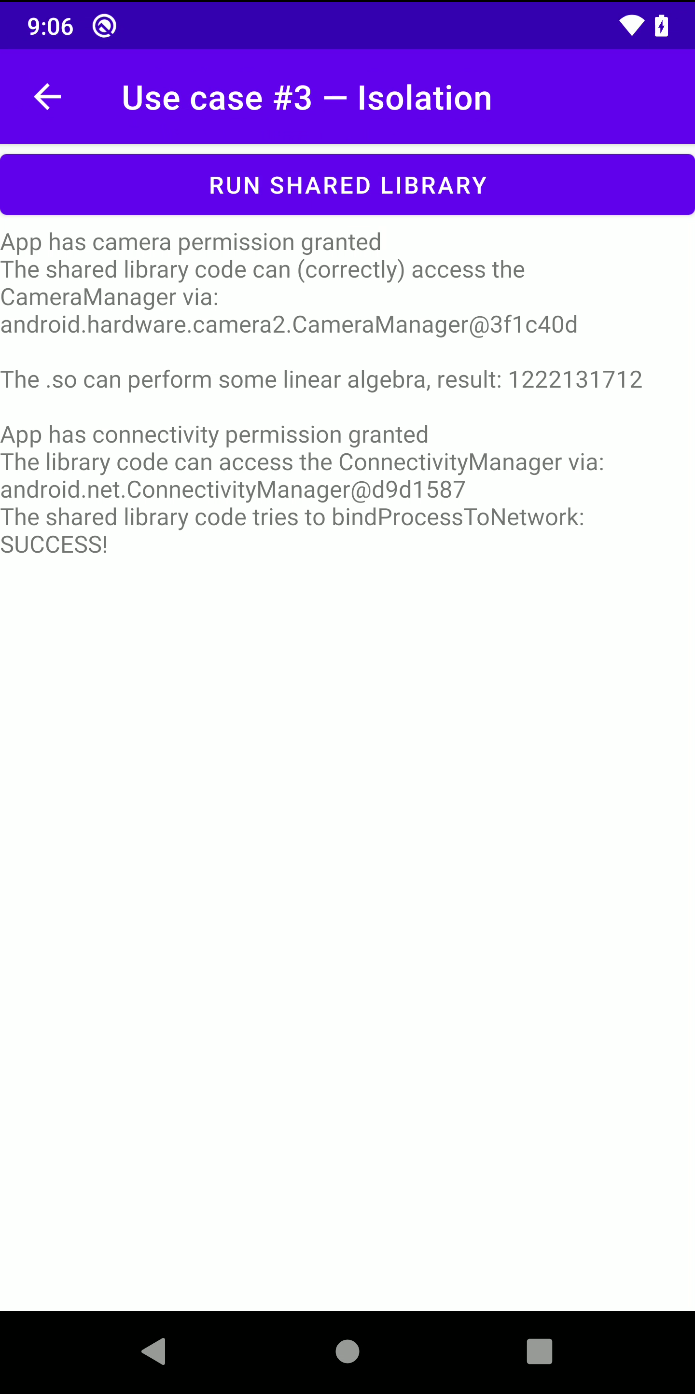
\includegraphics[width=0.3\textwidth]{chapters/seapp/figs/ae/uc32.png}}
  \hfill
  \subfloat{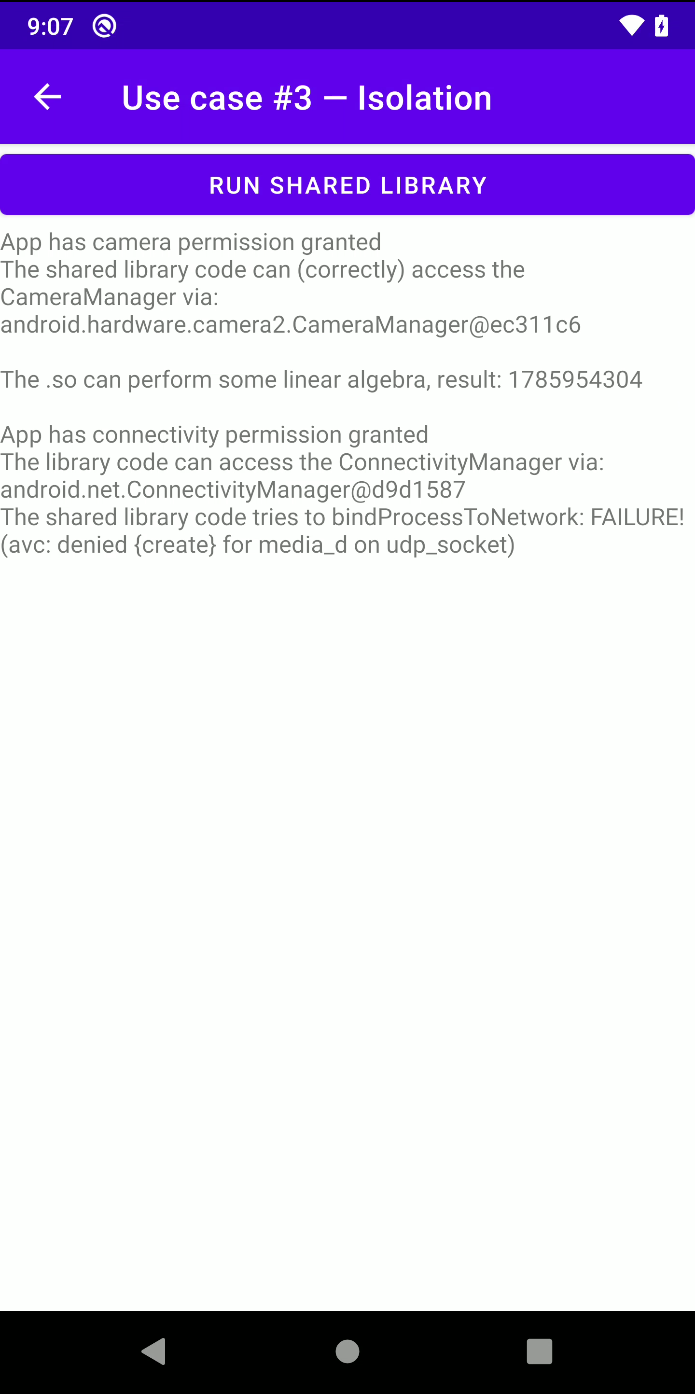
\includegraphics[width=0.3\textwidth]{chapters/seapp/figs/ae/uc33.png}}
  \caption{\label{fig:seapp_uc3_views} Use case 3 views}
\end{figure}

The native library is invoked by {\em UseCase3Activity}
(Figure~\ref{fig:seapp_uc3_views}a), which, according to line 4 in the
\seappcontexts, is executed in a process labeled with {\tt media\_d}
by {\em Zygote}.  The call to the library is performed via JNI. Its
job is to connect to the {\em camera\textunderscore service} and take
a picture.  Since the app is granted the {\em CAMERA} permission, the
native library code (legitimately, line 53 in the \sepolicy) connects
to the {\tt CameraManager}.

Since the native library performs image processing, we do not want it
to access the network. However, the permissions {\em INTERNET} and
{\em ACCESS\textunderscore NETWORK\textunderscore STATE} are granted
to the app, as they are required by the Ads framework.  Thus, when the
policy module is not available, the native library can connect to the
{\tt ConnectivityManager} and successfully bind the current process to
the network (Figure~\ref{fig:seapp_uc3_views}b).  Instead, when the
policy module is enforced by SEApp, since {\tt media\_d} was granted
only the basic app permissions (line 11 in \sepolicy), the connection
to the network is forbidden (Figure~\ref{fig:seapp_uc3_views}c).  This
happens because binding a process to the network is associated with
opening a network socket, an operation not permitted by \sel without
the required permissions. The following denial is written to the
system log: {\em denied {\tt create} on {\tt udp\textunderscore
    socket} to {\tt media\textunderscore d} domain}
(Figure~\ref{fig:seapp_uc3_logcat}).

\begin{figure}[h]
  \centering
  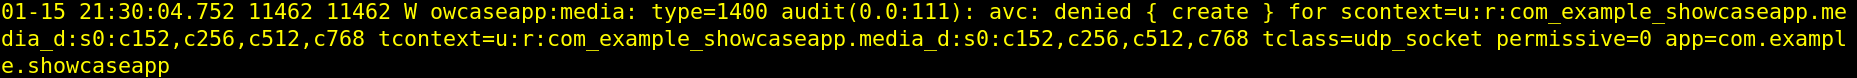
\includegraphics[width=\textwidth]{chapters/seapp/figs/ae/uc35.png}
  \caption{\label{fig:seapp_uc3_logcat} Use case 3 logcat - \sel denial}  
\end{figure}      

This use case, besides showing how SEApp confines a native library,
also demonstrates the power and simplicity of the macro, as adding the
line {\tt (call md\textunderscore netdomain (media\textunderscore d))}
to the policy module grants to {\tt media\textunderscore d} the needed
permissions to access the network.  The application developer is thus
not required to know or understand the internal \sel policy in order
to leverage this functionality.

The isolation properties introduced by \pap applies also to other
common security problems presented
in~\cite{seapp_common_play_protect_vulnerabilites}. Just to mention
one, \pap can mitigate the impact of incorrect sandboxing of a
scripting language.

%%% Local Variables: 
%%% mode: latex
%%% TeX-master: "../../../../main.tex"
%%% reftex-default-bibliography: "../../../../bib/biblio.bib"
%%% End:

\section[Policy module]{Showcase app policy module}\label{appendix:seapp_policy}

Here are reported the showcase app policy module files.
\vspace{0.6em}
\begin{lstlisting}[language=policyfile, caption=\bf showcase app
seapp\textunderscore contexts, captionpos=b, numbersep=2pt,
resetmargins=false, label=seapp_seappctxp]
user=_app seinfo=showcase_app domain=com_example_showcaseapp.core_logic_d name=com.example.showcaseapp:core_logic levelFrom=all
user=_app seinfo=showcase_app domain=com_example_showcaseapp.user_logic_d name=com.example.showcaseapp:user_logic levelFrom=all
user=_app seinfo=showcase_app domain=com_example_showcaseapp.ads_d name=com.example.showcaseapp levelFrom=all
user=_app seinfo=showcase_app domain=com_example_showcaseapp.media_d name=com.example.showcaseapp:media levelFrom=all
\end{lstlisting}
\vspace{0.6em}
\begin{lstlisting}[language=policyfile, caption=\bf showcase app
file\textunderscore contexts, captionpos=b,
numbersep=2pt,resetmargins=false, , label=seapp_filectxp]
.*                  u:object_r:app_data_file:s0
files/confidential  u:object_r:com_example_showcaseapp.confidential_t:s0
files/ads_cache     u:object_r:com_example_showcaseapp.ads_t:s0
\end{lstlisting}
\vspace{0.6em}
\begin{lstlisting}[language=policyfile, caption=\bf showcase app
mac\textunderscore permissions.xml, captionpos=b, numbersep=2pt, resetmargins=false, label=seapp_macctxp]
<?xml version="1.0" encoding="iso-8859-1"?>
<policy><signer signature="SIGNATURE">
<package name="com.example.showcaseapp">
<seinfo value="showcase_app"/></package>
</signer></policy>
\end{lstlisting}
\vspace{0.6em}
\begin{lstlisting}[language=policyfile, caption=\bf showcase app sepolicy.cil,
captionpos=b, numbersep=2pt, resetmargins=false, label=seapp_sepolctxp]
(block com_example_showcaseapp
; creation of domain types
(type core_logic_d)
(call md_untrusteddomain (core_logic_d))
(type user_logic_d)
(call md_appdomain (user_logic_d))
(type ads_d)
(call md_appdomain (ads_d))
(call md_netdomain (ads_d))
(type media_d)
(call md_appdomain (media_d))
(typeattribute domains)
(typeattributeset domains (core_logic_d user_logic_d ads_d media_d))
; creation of file types
(type confidential_t)
(call mt_appdatafile (confidential_t))
(type ads_t)
(call mt_appdatafile (ads_t))
; bounding the domains and types
(typebounds untrusted_app core_logic_d)
(typebounds untrusted_app user_logic_d)
(typebounds untrusted_app ads_d)
(typebounds untrusted_app media_d)	
(typebounds app_data_file confidential_t)
(typebounds app_data_file ads_t)
; grant core_logic_d access to confidential files
(allow core_logic_d confidential_t (dir (search write add_name)))
(allow core_logic_d confidential_t (file (create getattr open read write)))
; grant ads_d access to ads_cache files
(allow ads_d ads_t(dir(search write add_name)))
(allow ads_d ads_t(file(create getattr open read write)))
; minimum app_api_service subset
(allow domains activity_service (service_manager (find)))
(allow domains activity_task_service (service_manager (find)))
(allow domains ashmem_device_service (service_manager (find)))
(allow domains audio_service (service_manager (find)))
(allow domains surfaceflinger_service (service_manager (find)))
(allow domains gpu_service (service_manager (find)))
; grant core_logic_d the needed permissions
(allow core_logic_d restorecon_service (service_manager (find)))
(allow core_logic_d location_service (service_manager (find)))
; grant ads_d access to unity3ads needed services
(allow ads_d radio_service (service_manager (find)))
(allow ads_d webviewupdate_service (service_manager (find)))
(allow ads_d autofill_service (service_manager (find)))
(allow ads_d clipboard_service (service_manager (find)))
(allow ads_d batterystats_service(service_manager (find)))
(allow ads_d batteryproperties_service (service_manager (find)))
(allow ads_d audioserver_service (service_manager (find)))
(allow ads_d mediaserver_service (service_manager (find)))
; grant media_d the needed permissions
(allow media_d autofill_service (service_manager (find)))
(allow media_d cameraserver_service (service_manager (find))))
\end{lstlisting}


%%% Local Variables: 
%%% mode: latex
%%% TeX-master: "../../../main.tex"
%%% reftex-default-bibliography: "../../../bib/biblio.bib"
%%% End:
% natisand appendix
\chapter{Policy generated for the \texttt{curl} command}\label{appendix:curl_policy}

\vspace{-0.2mm}
Listing~\ref{lst:curl_policy_file} reports the policy associated with
the execution of the {\tt curl https://www.example.com} command. The policy has
been automatically generated using the utility described in
Section~\ref{sect:sci-ffi-policy-generation}.

\begin{lstlisting}[
    abovecaptionskip=-2pt,
    caption=Example of policy associated with curl,
    language=json,
    label=lst:curl_policy_file,
]
[{
  "name": "/usr/bin/curl",
  "fs": {
    "read": [
      "/etc/gai.conf",
      "/etc/host.conf",
      "/etc/hosts",
      "/etc/ld.so.cache",
      "/etc/localtime",
      "/etc/nsswitch.conf",
      "/etc/passwd",
      "/etc/resolv.conf",
      "/etc/ssl/certs/ca-certificates.crt",
      "/lib/x86_64-linux-gnu",
      "/lib64/ld-linux-x86-64.so.2",
      "/usr/bin/curl",
      "/usr/lib/locale/locale-archive",
      "/usr/lib/ssl/openssl.cnf"
    ],
    "exec": [
      "/lib/x86_64-linux-gnu",
      "/lib64/ld-linux-x86-64.so.2",
      "/usr/bin/curl"
    ]
  },
  "net": [{
    "name": "https://www.example.com",
    "ports": [443]
  }]
}]
\end{lstlisting}


% ------------------ BIBLIOGRAPHY ----------------- %

\bibliographystyle{abbrv}
\renewcommand\bibname{References}
\bibliography{biblio.bib}

\end{document}
